The second run period of the LHC, starting in 2015 at a centre of mass energy of $\sqrt{s} = 13$\tev, provides the excellent opportunity to further investigate the question if supersymmetry is realised in nature at the \tev scale. As discussed in Section~\ref{sec:susy_status}, the current limits exclude stop quarks with masses up to around 750\gev for LSP masses below 100\gev in case of direct stop production. Since for natural supersymmetry the stop quark mass is expected to not exceed 1\tev significantly, it is of particular interest to probe the stop mass range above 750\gev during the next run period of the LHC. The targeted process of this analysis is illustrated in a diagram in Fig.~\ref{fig:T2tt} below.  
\begin{figure}[!h]
  \centering
  \begin{tabular}{c}
                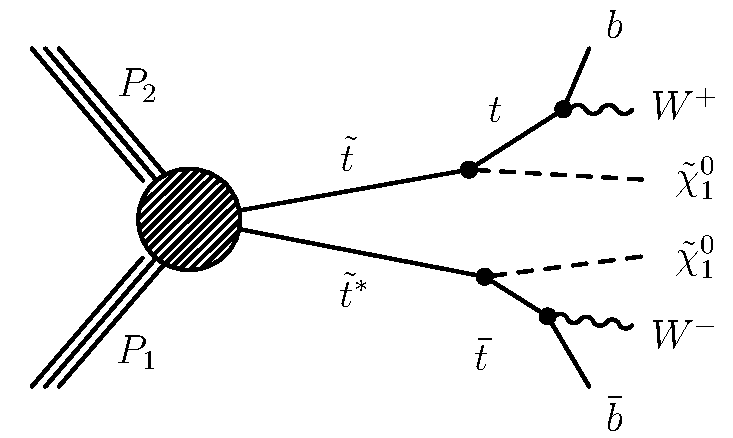
\includegraphics[width=0.68\textwidth]{figures/T2tt.pdf} 
  \end{tabular}
  \caption{Schematic diagram of the direct pair production of stop quarks in \pp collisions with subsequent decay into a top quark and the LSP. Taken from~\cite{bib:CMS:PhysicsResultsSUS}. }
  \label{fig:T2tt}
\end{figure}
\\   
Here, the pair production of stop quarks is shown with subsequent decay into a top quark and a neutralino LSP. Since each of the top quarks decays into a $b$ quark and a $W$ boson, the final state signature further depends on the decay modes of the $W$ bosons. In this analysis, only final states with fully hadronic top quark decays are considered. Consequently, this analysis targets a jet final state accompanied by missing transverse energy caused by the LSPs. As discussed in Section~\ref{subsec:susy_collider}, background contributions from the SM to such signatures arise mainly from QCD multijet events, \WJets, \ZJets and \ttbar events. \\
In this chapter, various analysis strategies for a search for stop quarks at $\sqrt{s} = 13$\tev are discussed and compared in order to address mass scenarios with large mass differences between the stop quark mass and the LSP. Furthermore, the performance of new selections is compared to the existing all-hadronic stop search performed by the CMS experiment at $\sqrt{s} = 8$\tev which is published in~\cite{CMS-PAS-SUS-13-015} and denoted \textit{SUS-13-015} in the following. In addition, it is interesting to study if selections that are developed for a search for direct stop production are also sensitive to gluino-mediated production of third generation quarks. 

\section{Data Samples}
\label{sec:stop_samples}
\begin{table}[!t]
%\fontsize{9 pt}{1.2 em}
%\selectfont
\centering
\caption{Overview of simulated background and signal samples used in the analysis and corresponding production cross sections.}
\makebox[\linewidth]{
\begin{tabular}{llcc}
\multicolumn{4}{c}{} \\
\toprule
   Process &  & $\sigma$ & Precision \\
   \midrule
   \midrule
   \ttbar & & 0.805 [nb] & NNLO \\
   \midrule
   \WJets & \HT = [0, 50]\gev  & 99.92 [nb] & LO \\
          & \HT = [50, 150]\gev  & 15.98 [nb] & LO \\
          & \HT = [150, 300]\gev  & 1.328 [nb] & LO \\
          & \HT = [300, $\infty$]\gev  & 0.169 [nb] & LO \\
   \midrule
   \ZJets & \HT = [0, 100]\gev & 22.0 [nb] & LO \\
          & \HT = [100, 300]\gev & 0.951 [nb]& LO \\
          & \HT = [300, $\infty$]\gev & 0.0396 [nb]& LO \\
   \midrule
   QCD multijet & \HT = [100, 250]\gev & 22\,930 [nb]& LO \\
                & \HT = [250, 500]\gev & 465 [nb] & LO \\
                & \HT = [500, 1000]\gev & 18.66 [nb] & LO \\
                & \HT = [1000, $\infty$]\gev & 0.536 [nb] & LO \\
   \midrule
   \midrule
   Stop-pair production & $m_{\tilde{t}}$ = 600\gev &  0.17460 [pb] & NLO \\
                        & $m_{\tilde{t}}$ = 700\gev &  0.06705 [pb] & NLO \\ 
                        & $m_{\tilde{t}}$ = 800\gev &  0.02833 [pb] & NLO \\ 
                        & $m_{\tilde{t}}$ = 900\gev &  0.01289 [pb] & NLO \\ 
                        & $m_{\tilde{t}}$ = 1000\gev & 0.00615 [pb] & NLO \\ 
                        & $m_{\tilde{t}}$ = 1100\gev & 0.00307 [pb] & NLO \\ 
   \midrule
   \midrule
   Gluino-pair production & $m_{\tilde{g}}$ = 1300\gev & 0.0211 [pb] & NLO \\
                          & $m_{\tilde{g}}$ = 1500\gev & 0.0064 [pb] & NLO \\ 
                          & $m_{\tilde{g}}$ = 1700\gev & 0.0021 [pb] & NLO \\ 
   \bottomrule
\end{tabular}}
\label{tab:stop_samples} 
\end{table}    
The studies presented in this chapter are based on simulated samples at $\sqrt{s} = 13$\tev. These are processed with the fast detector simulation and consider the pileup scenario as it was present at $\sqrt{s} = 8$\tev including out-of-time pileup according to a bunch spacing of 50\,ns. Although these are not the pileup conditions expected for $\sqrt{s} = 13$\tev, the selections studied here typically are based on objects with high transverse momenta such that influences from pileup are negligible in good approximation. Moreover, the studies presented in this chapter are focusing on the identification of general analysis strategies comparing the relative performance of different selections, such that also simplifications caused by the use of the fast detector simulation are not explicitly accounted for. Some discussion about the impact of these simplifications concerning the analysis sensitivity follows in Sec.~\ref{sec:stop_results}.  \\
The processes considered in the analysis are summarized in Tab.~\ref{tab:stop_samples}. \WJets, \ZJets and QCD multijet events are generated with \textsc{Madgraph5}~\cite{Alwall:2014hca} using the PDF CTEQ6L1~\cite{Pumplin:2002vw}, while \ttbar events are generated with \powheg~\cite{Oleari:2010nx} and the MSTW2008 PDF~\cite{Martin:2009iq}. For all samples, the showering process is performed with \textsc{Pythia6}~\cite{Sjostrand:2006za} Tune Z2*~\cite{Chatrchyan:2013gfi}. The process \WJets includes decays with $W \rightarrow l \nu$ with up to two jets modelled in the matrix element. Similarly, also the process \ZJets includes up to two jets. Here, decays $Z \rightarrow \nu \nu$ are modelled. For these two processes, cross sections at NLO are obtained by applying scale factors computated with \powheg to the leading order cross sections. These scale factors amount to 1.04 and 1.07 for \WJets and \ZJets, respectively. The cross section calculation for \ttbar events is obtained from \textsc{Hathor}~\cite{Aliev:2010zk}. \\
In order to study signal events, two different processes are generated with \textsc{Madgraph5} and showered with \textsc{Pythia6}. On the one hand direct stop-pair production is considered in which the $\tilde{t}$ always decays to a stable neutralino $\tilde{\chi}_{0}^{1}$ and a top quark with mass $m_{t} = 172.5$\gev including all decay channels of the top quark. These samples are generated for stop masses listed in Tab.~\ref{tab:stop_samples} for different neutralino masses of 50, 100, 150, 200, 250, 300 and 350\gev. On the other hand gluino-pair production is generated with a decay $\tilde{g} \rightarrow \ttbar \tilde{\chi}_{0}^{1}$. For the top quark, only fully hadronic decays are simulated. The cross section given in Tab.~\ref{tab:stop_samples} for gluino-pair production is corrected for the hadronic branching fraction of the top quark. In this case, the neutralino mass is fixed to 50\gev. \\
All samples are normalized to an integrated luminosity of 19.5\fbinv which corresponds to the same integrated luminosity as recorded at $\sqrt{s} =8$\tev.

\section{Sensitivity of a Basic Selection using \HT and \met}
\label{sec:stop_baseline}
The targeted signature of the direct pair production of stops in the all-hadronic channel is based on jets and missing transverse momentum similar to the search presented in Chap.~\ref{chap:RA2}. Thus, a very similar baseline selection is employed as a basis for further studies. If not stated otherwise, jets are clustered with the anti-$k_\mathrm{T}$ algorithm and a distance parameter $R = 0.5$ including charged-hadron subtraction. Since no dedicated jet energy corrections for $\sqrt{s} = 13$\tev have been determined, jets are corrected with the respective correction factors for $\sqrt{s} = 8$\tev. The applied analysis criteria are:
\begin{itemize}
 \item{Background contributions arising from \ttbar and \WJets events are reduced by rejecting events containing isolated electrons or muons with $\pt > 10$\gev and $|\eta| < 2.5$. These are required to have a good quality track that can be associated with the primary interaction vertex~\cite{CMS-PAS-EGM-10-004, CMS-PAS-MUO-10-002}. The isolation is given as the scalar sum of transverse momenta of PF particles (except for the lepton itself) within a cone of width $\Delta R = 0.3$ for the electron and $\Delta R = 0.4$ for the muon, respectively, and is required to be less than 20\% of the transverse momentum of the electron and less than 15\% of the transverse momentum of the muon.}
 \item{The number of jets (\NJets) is required to be $\ge 3$. \NJets is defined as the number of jets with $\pt > 50$\gev and $|\eta| < 2.5$. This requirement is imposed in order to select multijet events as expected from the decays of the two top quarks.}
 \item{The scalar sum of jet momenta (\HT) is required to be $\ge 500$\gev with 
\begin{equation*}
\HT = \sum_{\mathrm{jets}} \pt 
\end{equation*}
for all jets with $\pt > 50$\gev and $|\eta| < 2.5$. This condition selects events with a large visible energy in the event indicating a high energy scale of the hard interaction.}   
 \item{The missing transverse energy \met calculated from the PF candidates is required to be $\ge 200$\gev. This selection reduces contributions from standard model processes in which missing transverse momentum is expected to be small. Especially, QCD multijet background is suppressed. } 
 \item{In order to suppress events in which missing transverse energy is mainly arising from jet mismeasurements, as for QCD multijet events, it is required that \met is not aligned with any of the leading three jets. Thus, events with
\begin{equation*}
\Delta \phi(\mathrm{jet}_n, \met) > 0.5 \;\; \mathrm{for} \;\; n = 1,2 \;\; \mathrm{and} \;\; \Delta \phi(\mathrm{jet}_3, \met) > 0.3
\end{equation*} 
are selected. The value of 0.5 is chosen according to the jet size parameter. However, this is reduced in case of the third jet in order to retain signal efficiency. }
\end{itemize}
Since only simulated events are used, no dedicated event cleaning filters are applied as it is necessary for data (cf. Sec~\ref{subsec:RA2_cleaning}). The selection described here is again denoted \textit{baseline selection} in the following. In Fig.~\ref{fig:stop_baseline}, the obtained spectra of \HT, \met and \NJets after applying the baseline selection are shown for the SM backgrounds and two selected signal points normalized to an integrated luminosity of 19.5\fbinv. The signal points represent mass values of 600\gev and 1100\gev for the stop mass while the LSP mass is in both cases 50\gev. These two signal points illustrate the difference in the kinematic properties of events for low and high stop masses. Typically, the \HT and \met spectrum get harder for higher stop masses while the shape of the \NJets spectrum stays nearly unchanged. After applying baseline selection criteria, the background is composed almost equally of all four SM processes (\ttbar: 27\%, \WJets: 21\%, \ZJets:19\%, QCD: 33\%).
\begin{figure}[!t]
  \centering
  % \makebox[\linewidth]{
  \begin{minipage}[c]{1.\textwidth}
    \begin{center}
      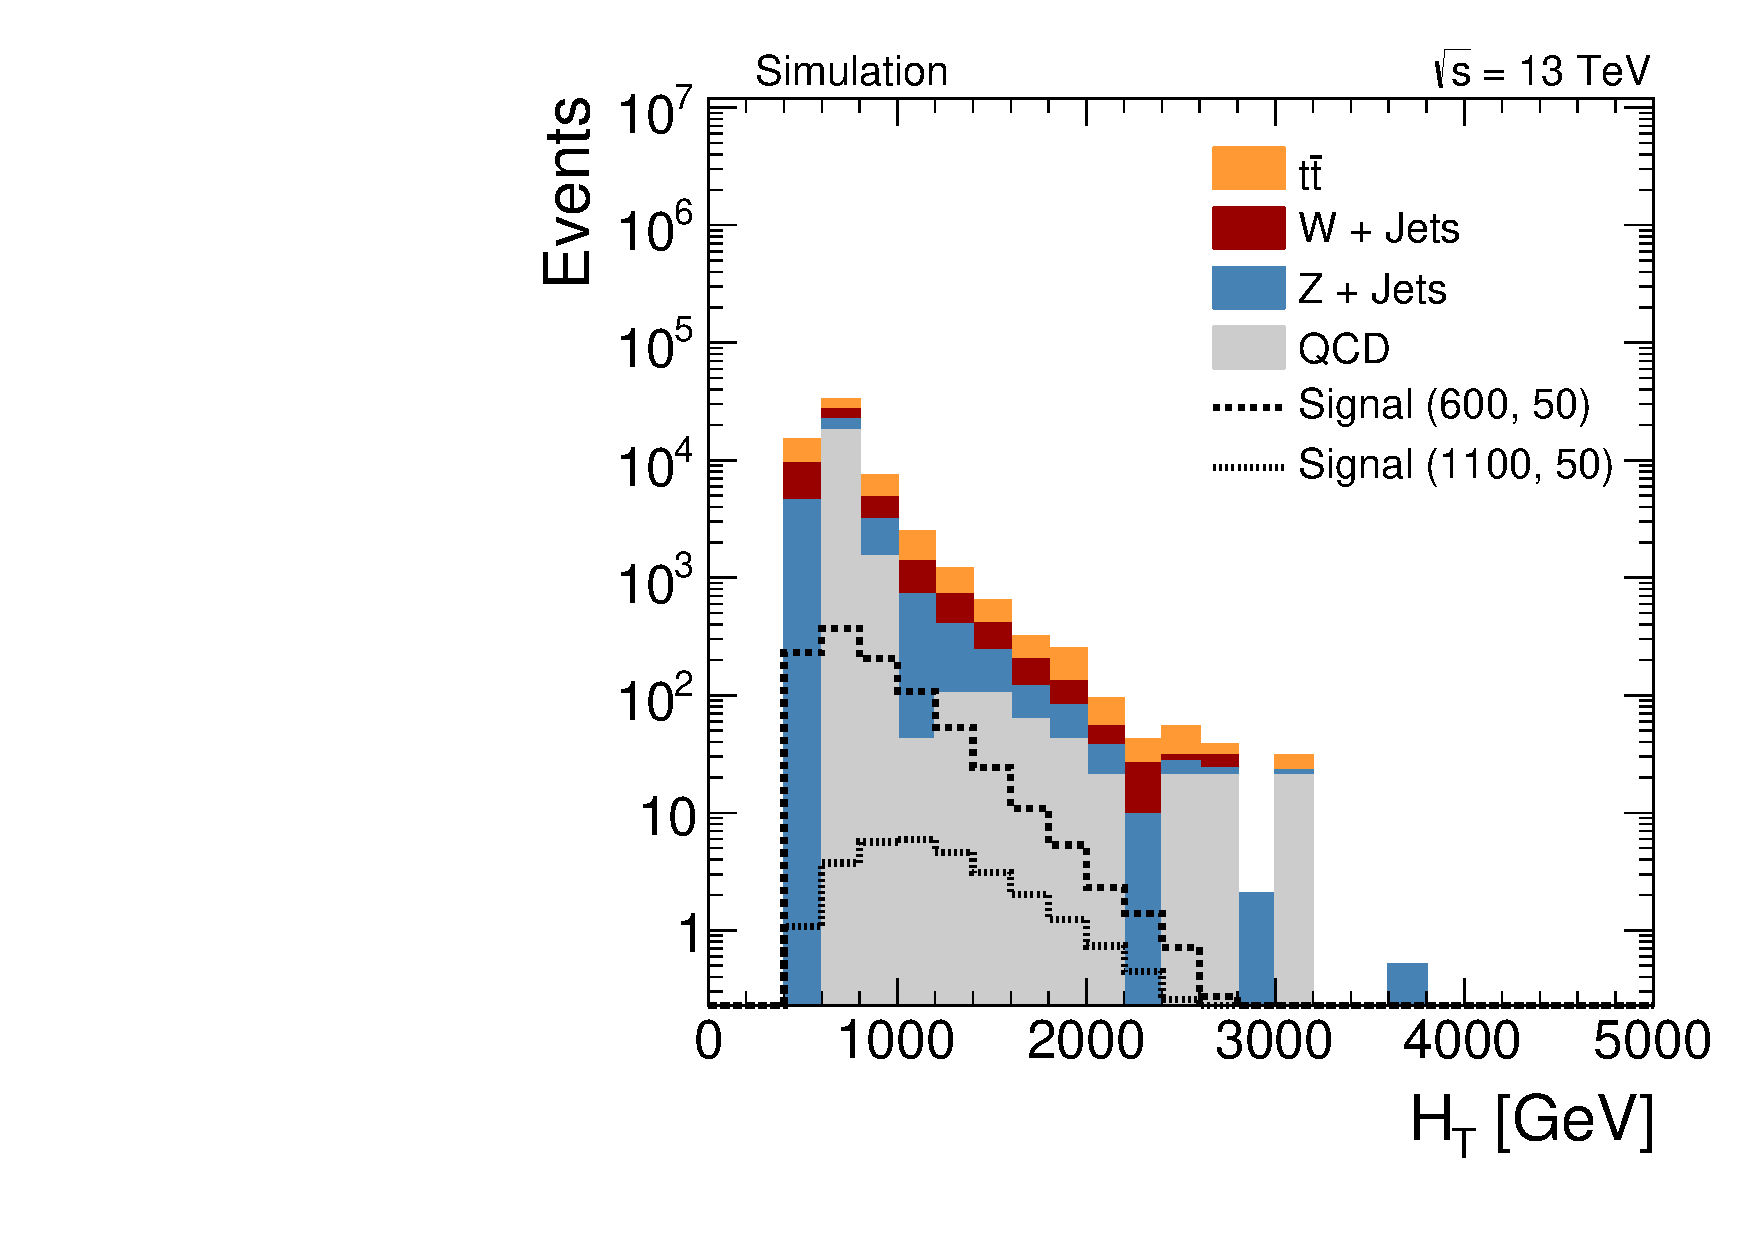
\includegraphics[width=0.49\textwidth]{figures/Stop_DeltaPhiSelection_HThad.pdf}  
      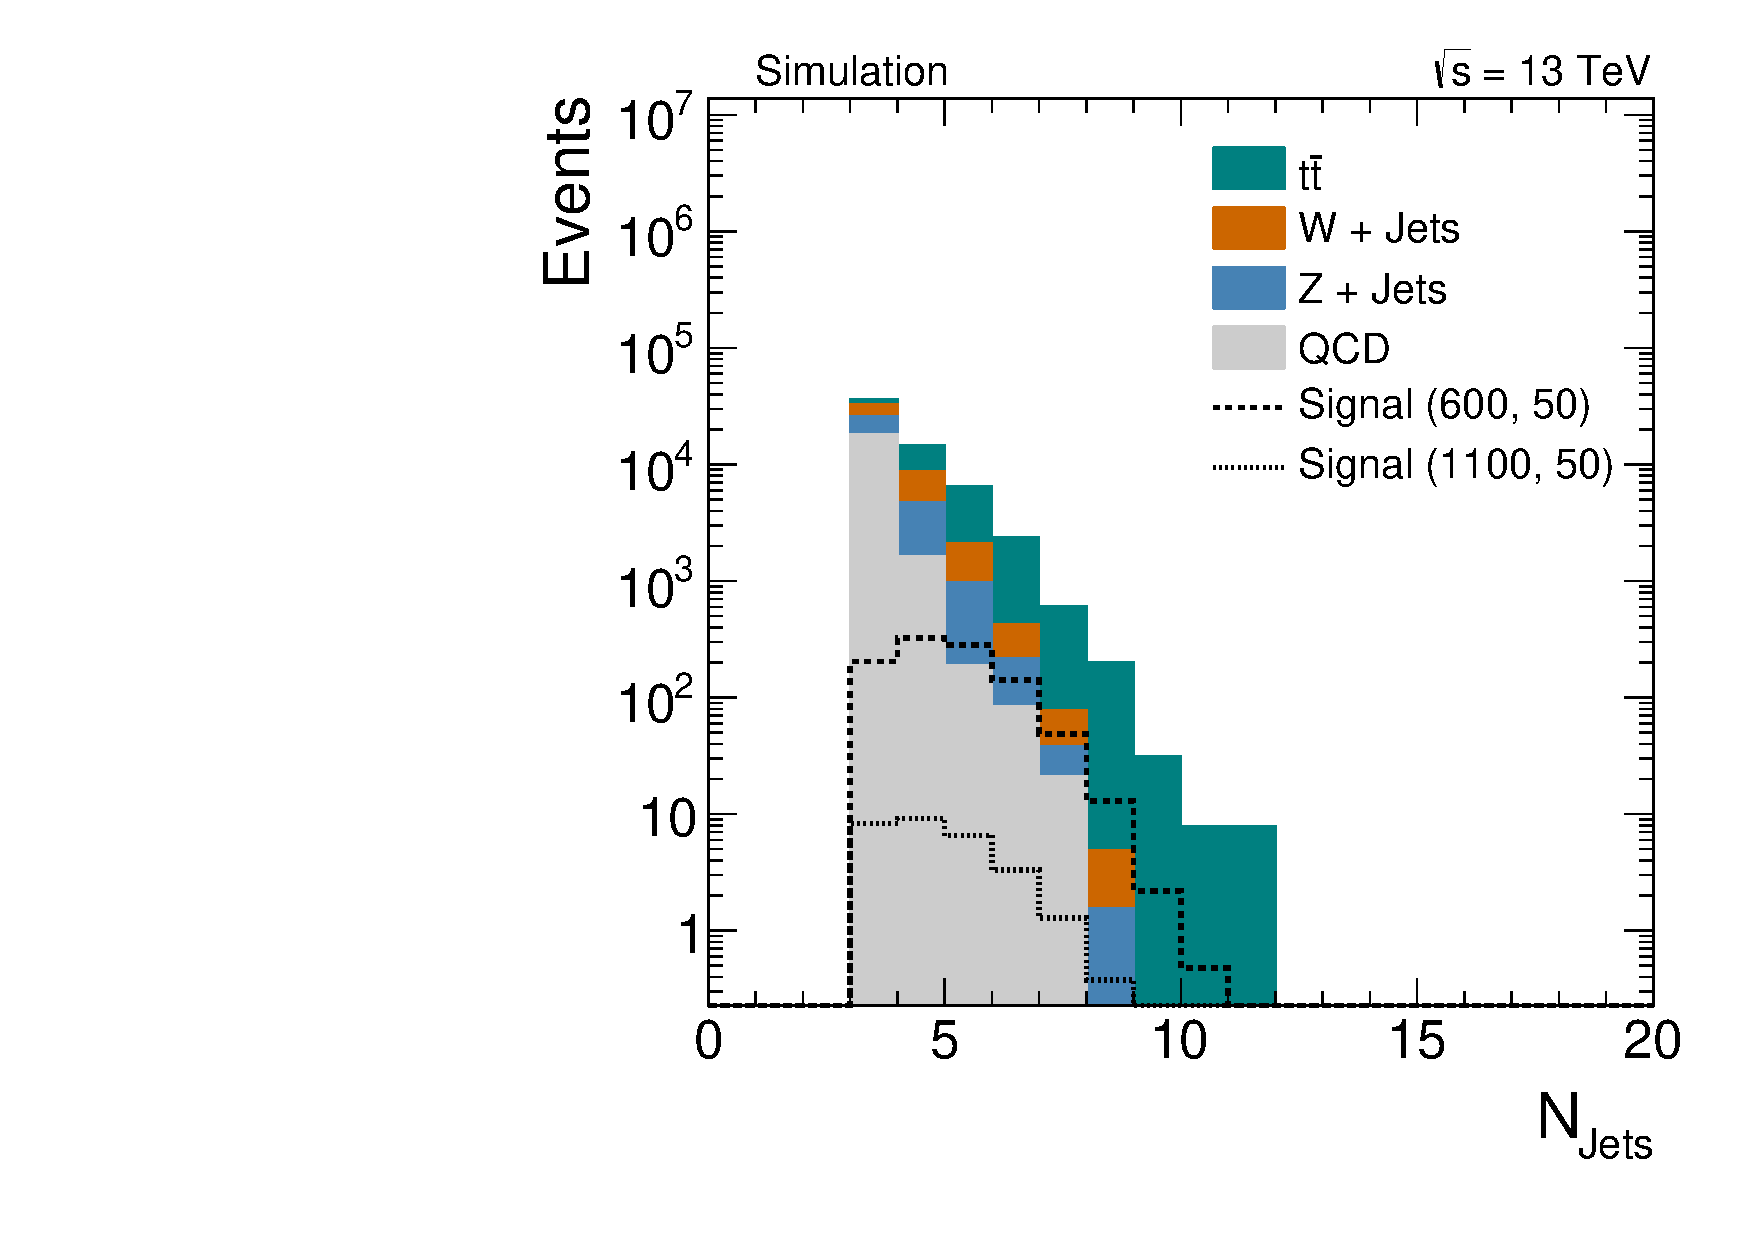
\includegraphics[width=0.49\textwidth]{figures/Stop_DeltaPhiSelection_N_jets.pdf} \\
      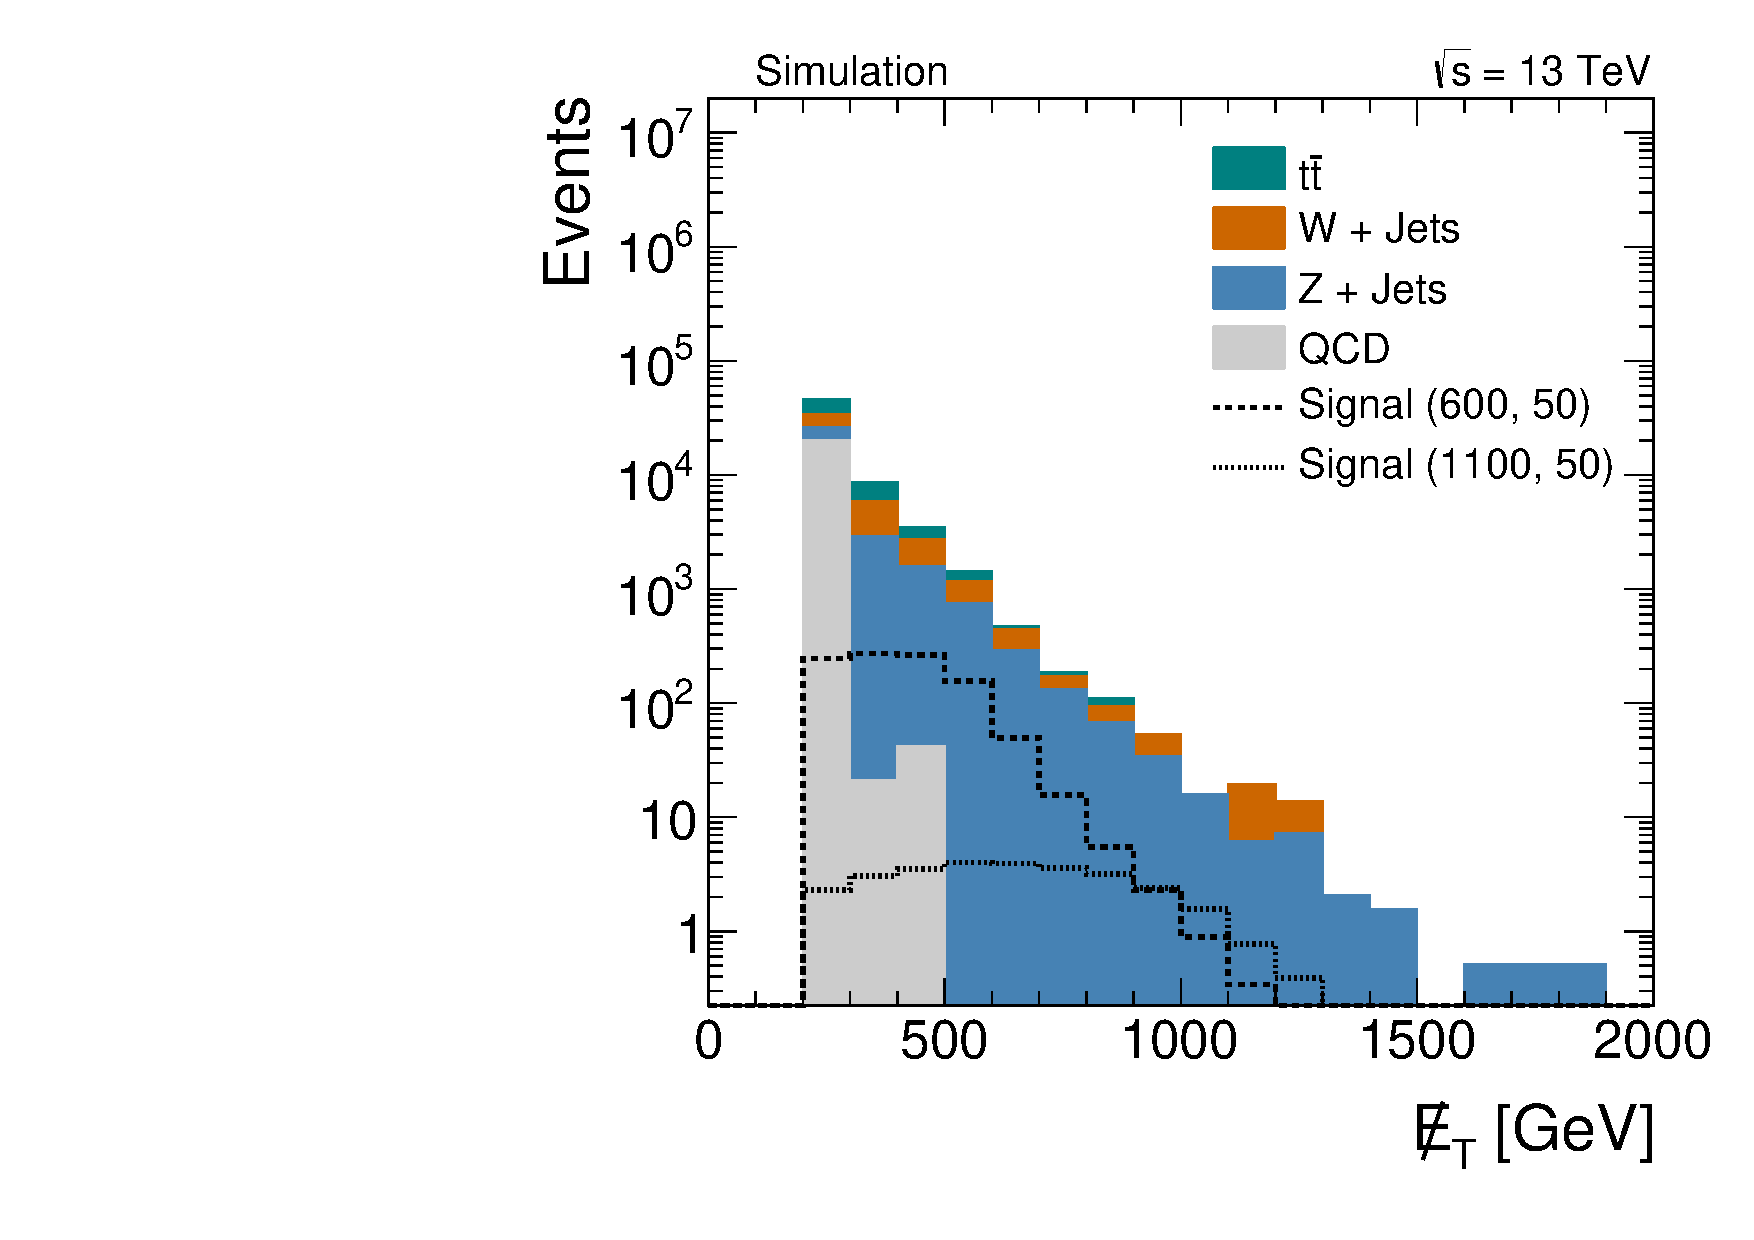
\includegraphics[width=0.49\textwidth]{figures/Stop_DeltaPhiSelection_MET.pdf} 
   %   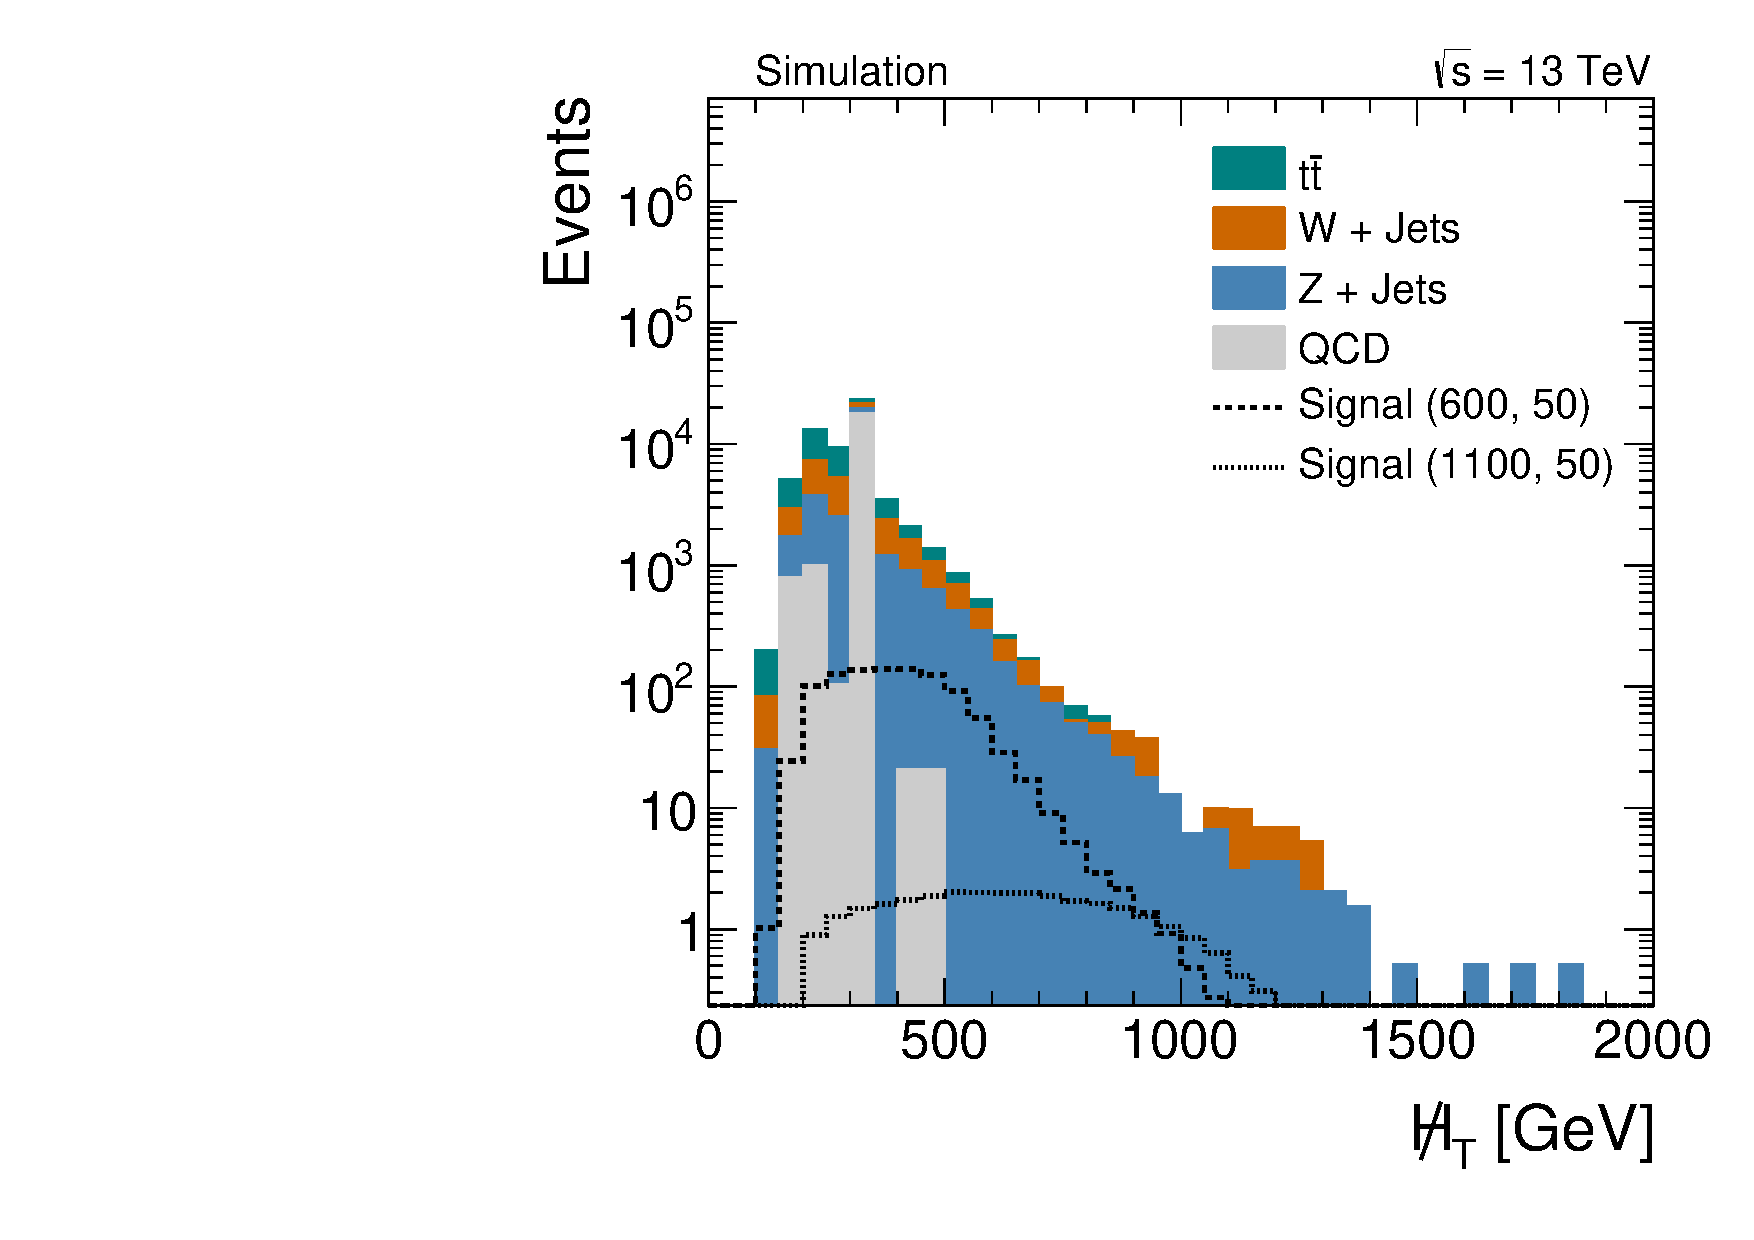
\includegraphics[width=0.49\textwidth]{figures/Stop_DeltaPhiSelection_MHT.pdf} 
    \end{center}
  \end{minipage}

  \caption{Comparison of selected \HT (\textit{top left}), \met (\textit{top right}) and \NJets (\textit{bottom}) distributions in simulated events found from applying the baseline selection criteria. The signal points are labelled as (X, Y) where X is the stop quark mass and Y is the LSP mass in GeV.}
  \label{fig:stop_baseline} 
\end{figure}
\\
In order to investigate how this baseline selection can be further improved to gain sensitivity to the model of interest, the evolution of the signal and background efficiencies is studied when changing specific selections in the analysis. In general, the signal and background selection efficiencies $\epsilon_\mathrm{sig/bg}$ are defined according to
\begin{equation}
\epsilon = \frac{\mathrm{no. \; of \; selected \; events}}{\mathrm{no. \; of \; all \; events}}
\end{equation} 
\begin{figure}[!t]
  \centering
\makebox[\linewidth]{
  \begin{tabular}{cc}
                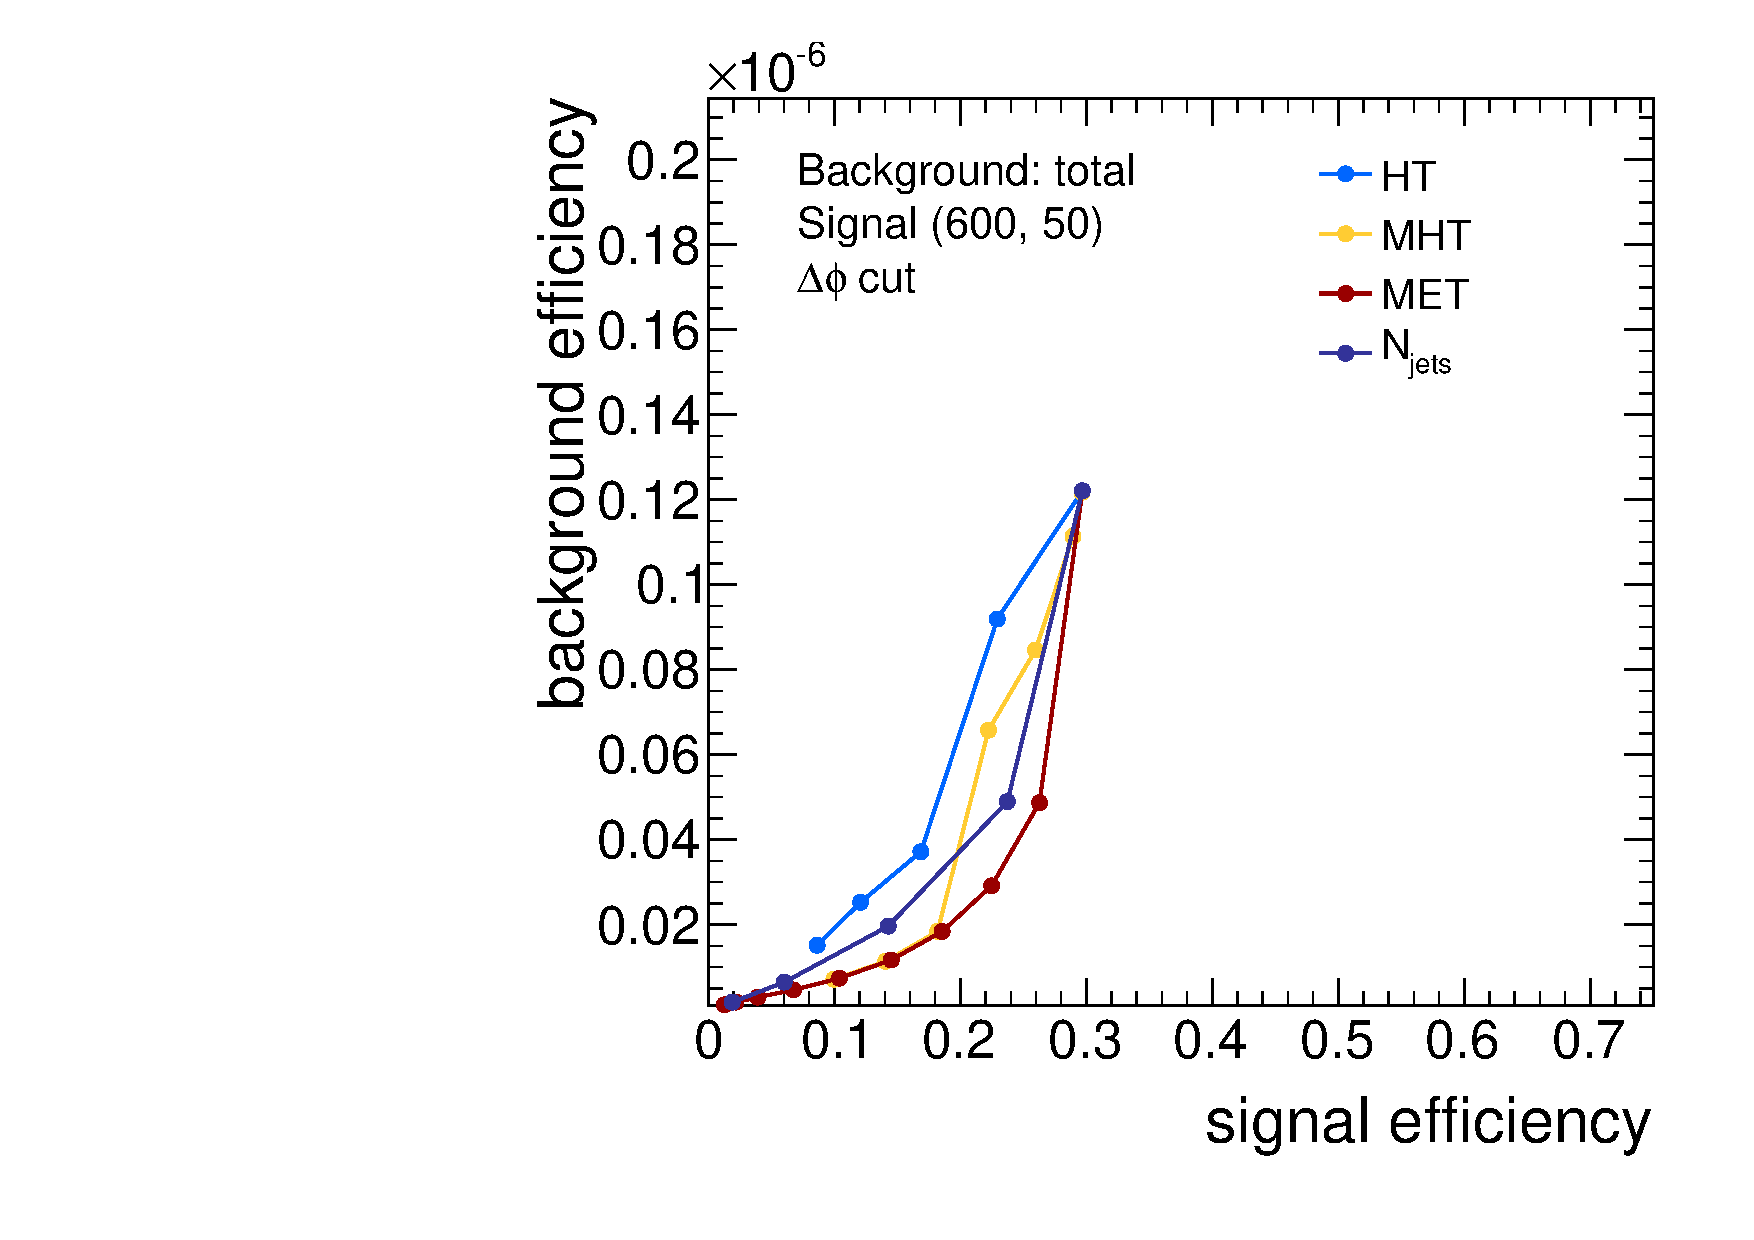
\includegraphics[width=0.49\textwidth]{figures/CutScan_DeltaPhiSelection_total_Stop600_LSP50_T2tt_13TeV_HT_MET_MHT_NJets.pdf} & 
                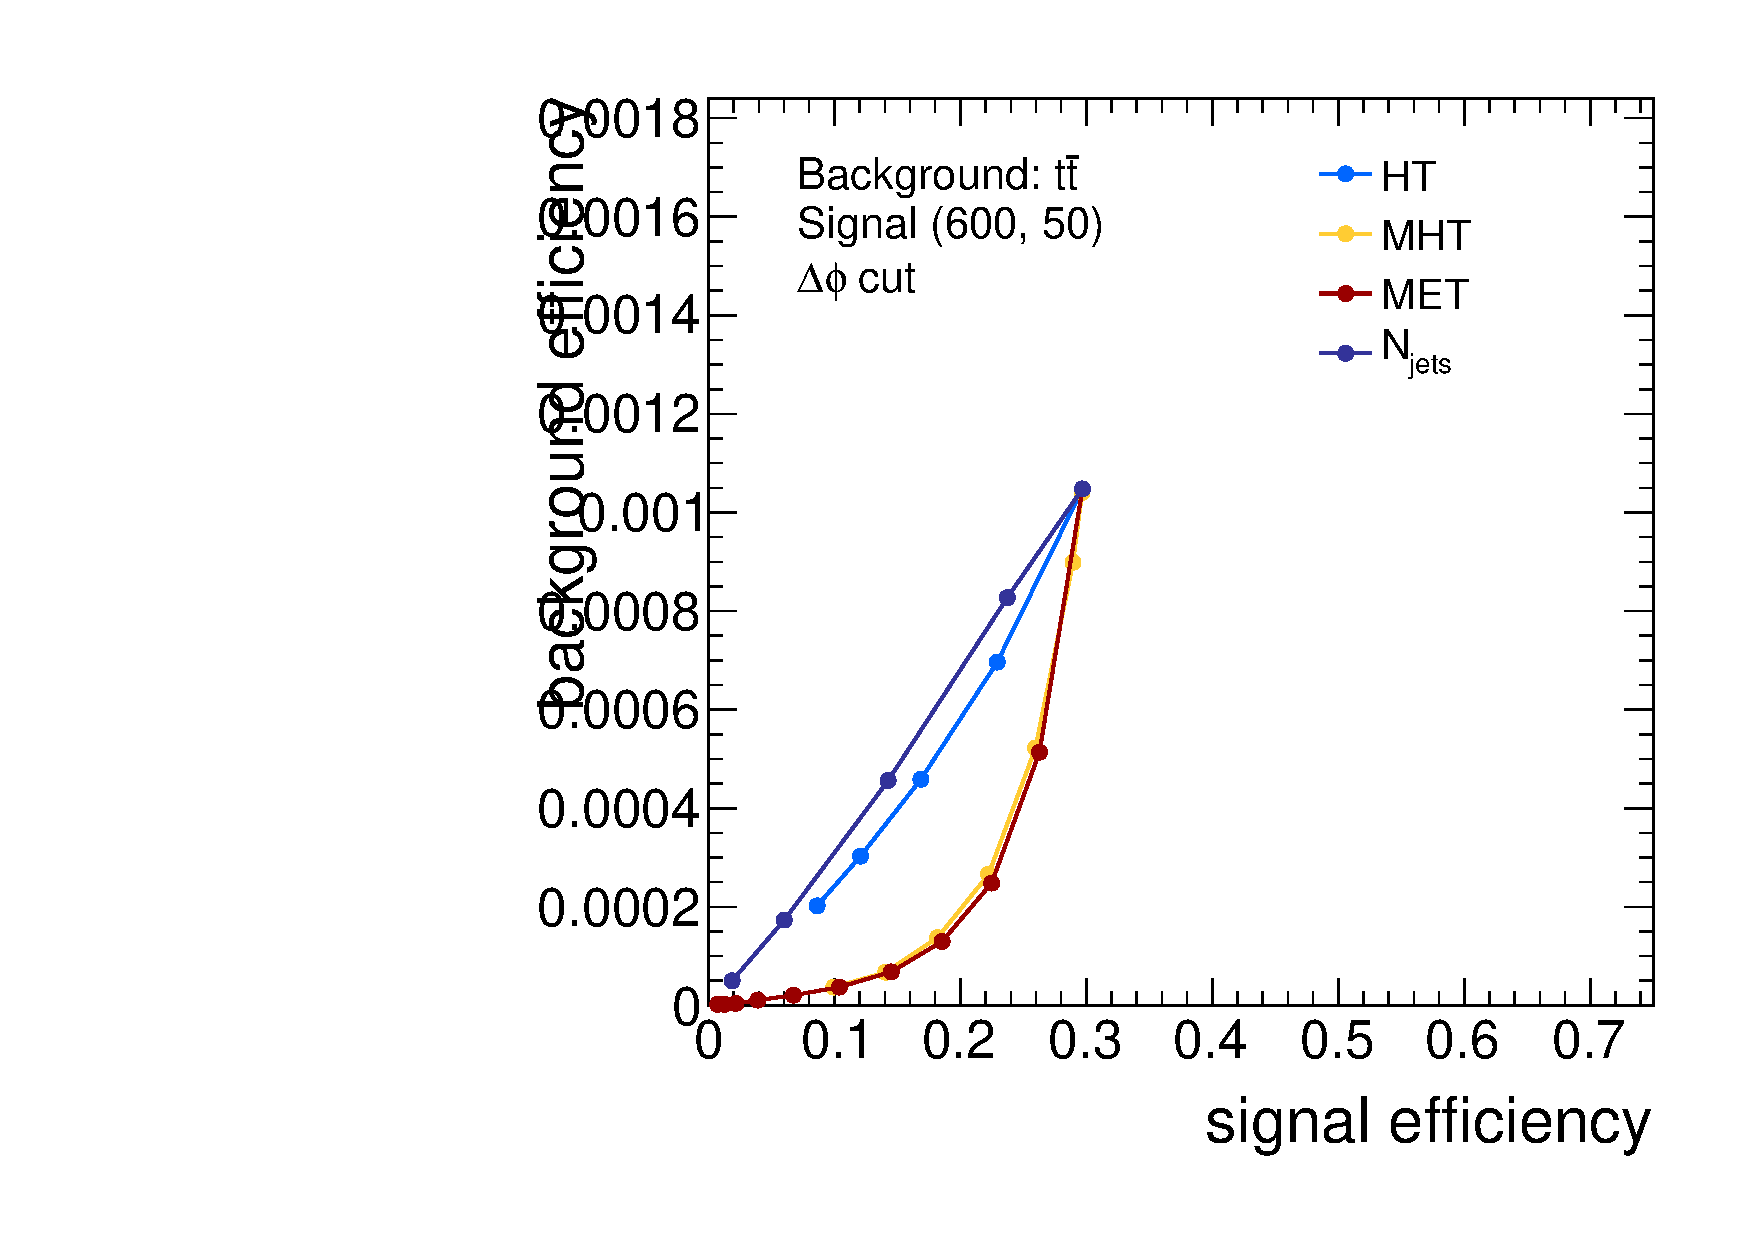
\includegraphics[width=0.49\textwidth]{figures/CutScan_DeltaPhiSelection_TTbar_powheg_13TeV_Stop600_LSP50_T2tt_13TeV_HT_MET_MHT_NJets.pdf} \\
                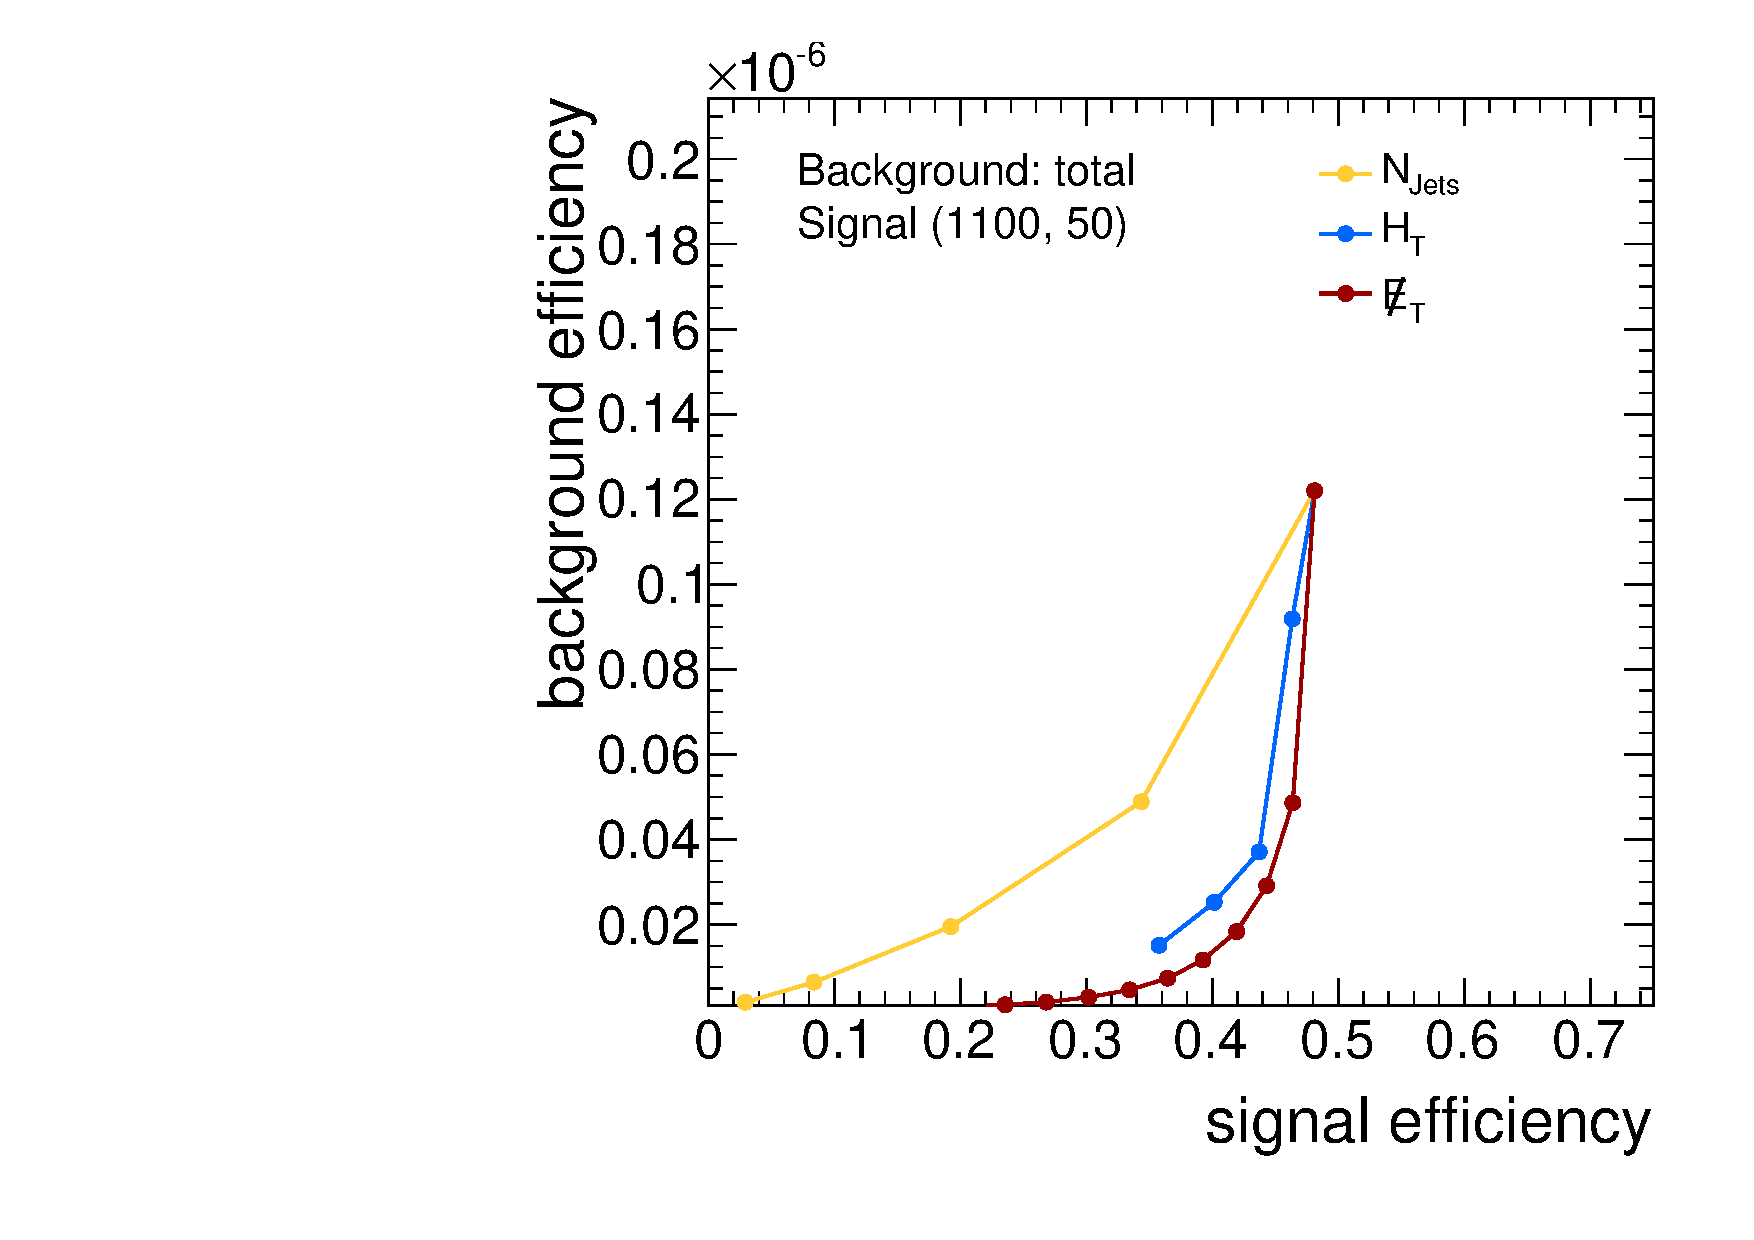
\includegraphics[width=0.49\textwidth]{figures/CutScan_DeltaPhiSelection_total_Stop1100_LSP50_T2tt_13TeV_HT_MET_MHT_NJets.pdf} &
                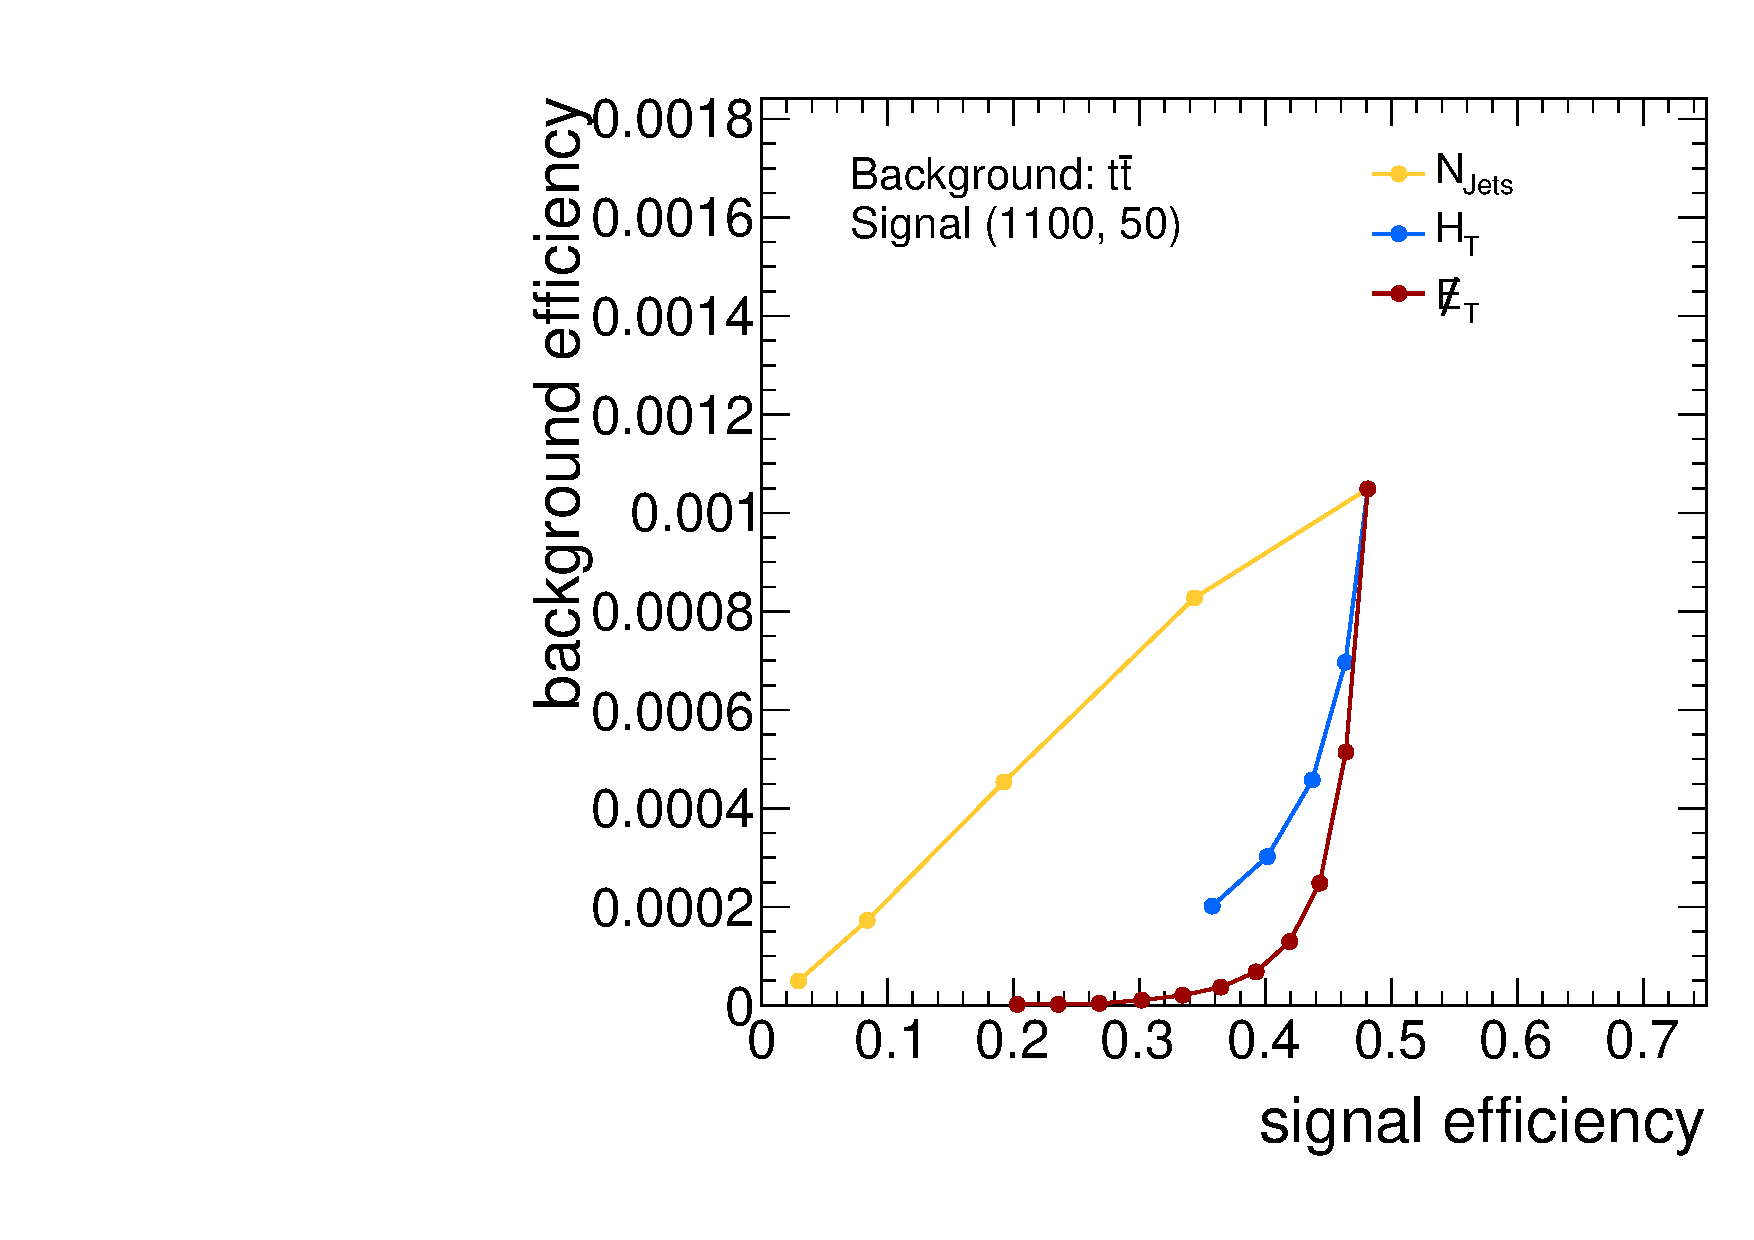
\includegraphics[width=0.49\textwidth]{figures/CutScan_DeltaPhiSelection_TTbar_powheg_13TeV_Stop1100_LSP50_T2tt_13TeV_HT_MET_MHT_NJets.pdf}
  \end{tabular}}
  \caption{Evolution of the signal versus background efficiency for a stop mass of 600\gev (\textit{top}) and 1100\gev (\textit{bottom}) in case the background is the sum of all backgrounds (\textit{left}) or only the \ttbar background (\textit{right}) after applying baseline selection criteria.}
  \label{fig:stop_baseline_cutscan_ht_met_mht_njets}
\end{figure}
for the number of signal and background events, respectively. In Fig.~\ref{fig:stop_baseline_cutscan_ht_met_mht_njets}, the evolution of the signal versus background efficiencies is shown for the stop mass 600\gev and 1100\gev signal points and \ttbar as well as total background events. The curves are obtained from increasing the cut value for the denoted variable by keeping the selection for all other variables fixed. The curve of a variable with good separation power runs close to the lower right corner. Here, the performance of \HT, \met and \NJets is compared. %In addition to \met, also \MHT, as defined in Sec.~\ref{subsec:RA2_baseline}, is shown in this comparison. Both variables show a very similar performance such that in principle both variables could be employed with similar results. However, the performance of \met seems to be slightly better and thus this variable is used in these studies rather than \MHT. Furthermore, as stated above, the same trigger as for the analysis presented in Chapter~\ref{chap:RA2} could be used to collect the data. Since this trigger is based on \met, the choice of the offline selections is closer to the online definition when using \met instead of \MHT.
As can be seen in Fig.~\ref{fig:stop_baseline_cutscan_ht_met_mht_njets}, variations of the \met selection show in general the best performance when comparing these variables. This holds for low and high stop masses as well as for the total background and when considering \ttbar background only. Furthermore, also \HT provides a good separation power and is only in case of the stop mass of 600~\gev inferior to \NJets when considering the total background. However, when only \ttbar background is considered, the jet multiplicity is not suitable as discriminating variable since the \NJets spectra of signal and \ttbar background are almost identical. As in general the kinematic features of \ttbar background are closest to the signal, it is of special importance to identify selections that can reduce this background. Consequently, \met and \HT are the preferred variables to distinguish signal and background processes. 
\\
In the following, an analysis strategy close to the one described in Chap.~\ref{chap:RA2} is pursued. Events selected with the baseline selection are further categorized according to their \HT and \met values in exclusive search regions shown in Tab.~\ref{tab:stop_excl_search_bins}. The event yields of background and two signal processes obtained after applying baseline requirements are shown for these different signal regions as well as for the total selected sample in Tab.~\ref{tab:stop_baseline_cutflow}. Furthermore, also the signal over background ratios are displayed. In general, the signal to background ratio in SR1 is very low such that this bin is not expected to contribute to the search sensitivity significantly, but can be used to constrain the background estimate. As seen already from the signal versus background efficiency curves, the best discrimination between signal and background events can be obtained by selecting high values of \met (SR2 and SR4), while the overall best sensitivity is given when combining the high \met selection also with the high \HT selection (SR4). However, the signal to background ratios in all search regions are so low that it is not expected to be able to really probe the considered stop mass scenarios with such a basic selection. 
\begin{table}[!t]
%\fontsize{10 pt}{1.2 em}
%\selectfont
\centering
\caption{Exclusive search regions (SR) used in the analysis binned in \HT and \met.}
\begin{tabular}{lll}
\multicolumn{3}{c}{} \\
  \toprule
  SR1 &  $500 < \HT < 1000$\gev  & $200 < \met < 400$\gev  \\                  
  \midrule
  SR2 &  $500 < \HT < 1000$\gev  & $400\gev < \met$  \\ 
  \midrule 
  SR3 &  $1000\gev < \HT$  & $200 < \met < 400$\gev  \\ 
  \midrule     
  SR4 &  $1000\gev < \HT$  & $400\gev < \met$  \\                
  \bottomrule
\end{tabular}
\label{tab:stop_excl_search_bins}
\end{table}  
\\ 
\\
In order to get an even better estimate of the search sensitivity than from the signal to background ratios of the individual search regions, the sensitivity of a certain selection is quantified by determining the expected exclusion reach. While the signal to background ratios are useful to get a general impression of the selection quality, the expected exclusion reach combines the information from all search regions and thus provides a more accurate estimate of the search sensitivity. Thus, it is used in the following to quantify the quality of a certain selection and compare it to others. \\
In order to determine the exclusion reach, the uncertainties of the individual background processes have to be considered. These are not explicitly estimated but chosen in correspondence to the uncertainties obtained for similar kinematic regimes in SUS-13-015. The respective uncertainties taken into account for the different processes are
\begin{itemize}
 \item QCD multijet events: 100\%
 \item \ZJets: 50\%
 \item \WJets: 20\%
 \item \ttbar: 20\% + additional 20\% in the high \met search regions (SR2, SR4)
\end{itemize}  
These are treated as total uncertainties which means that the relative rate is assumed to be known for the first three backgrounds and allowed to vary within the additional 20\% for \ttbar background. The actual statistical uncertainty of the number of simulated MC events is not considered explicitly. 
\begin{table}[!t]
%\fontsize{9 pt}{1.2 em}
%\selectfont
\centering
\caption{Total event yields obtained from simulated samples after the baseline selection described in the text (\textit{first column}) as well as event yields for the various signal regions (\textit{column two to five}). All numbers are scaled to 19.5\fbinv. The signal points are labelled as (X, Y) where X is the stop quark mass and Y is the LSP mass in GeV. Furthermore, the signal over background ratios are displayed for the two signal points in squared brackets. }
 \resizebox{\textwidth}{!}{%
%\makebox[\linewidth]{
\begin{tabular}{llllll}
\multicolumn{6}{c}{} \\
  \toprule
    & total & SR1 & SR2 & SR3 & SR4  \\
  \midrule
   \ttbar & 16461 & 13525 & 754 & 1868 & 314 \\
   \WJets & 12481 & 9660 & 1516 & 985 & 320 \\
   \ZJets & 11837 & 8155 & 2425 & 810 & 447 \\
   QCD multijet & 20013 & 19574 & 0 & 397 & 42 \\
   \midrule
   Signal (600, 50) & 1012 [16.6$\cdot 10^{-3}$] & 416 [8.2$\cdot 10^{-3}$] & 389 [82.8$\cdot 10^{-3}$] & 101 [24.9$\cdot 10^{-3}$] & 106 [94.6$\cdot 10^{-3}$]  \\
   Signal (1100, 50) & 29 [0.5$\cdot 10^{-3}$] & 2 [0.05$\cdot 10^{-3}$] & 8 [1.7$\cdot 10^{-3}$] & 3 [0.7$\cdot 10^{-3}$] & 16 [14.0$\cdot 10^{-3}$]  \\
  \bottomrule
\end{tabular}}
\label{tab:stop_baseline_cutflow}
\end{table}   
\\
Based on the selected event yields and the estimated uncertainties, the 95\% confidence-level expected upper limit is calculated as an asymptotic $\mathrm{CL_s}$ limit~\cite{bib:theta}. The obtained exclusion curve is shown in Fig.~\ref{fig:stop_baseline_limit} for the signal strength $\mu$ which is the excluded production cross section divided by the theoretical cross section for direct stop production as a function of the stop quark mass.\footnote{As stated in the beginning, the main focus of these studies lies on scenarios with large mass differences between stop quark and LSP. Thus, the LSP mass is fixed to 50\gev here. The sensitivity of the analysis towards other LSP masses is discussed later in Sec.~\ref{sec:stop_results}.} A particular mass point can be excluded if the expected limit drops below one. As expected from the signal to background ratios, this baseline selection cuts and the subsequent binning in exclusive search regions is not yet sensitive enough to probe any of the selected mass points. Thus, possible improvements of the analysis are discussed in the following sections.  
\begin{figure}[!h]
  \centering
  \begin{tabular}{c}
                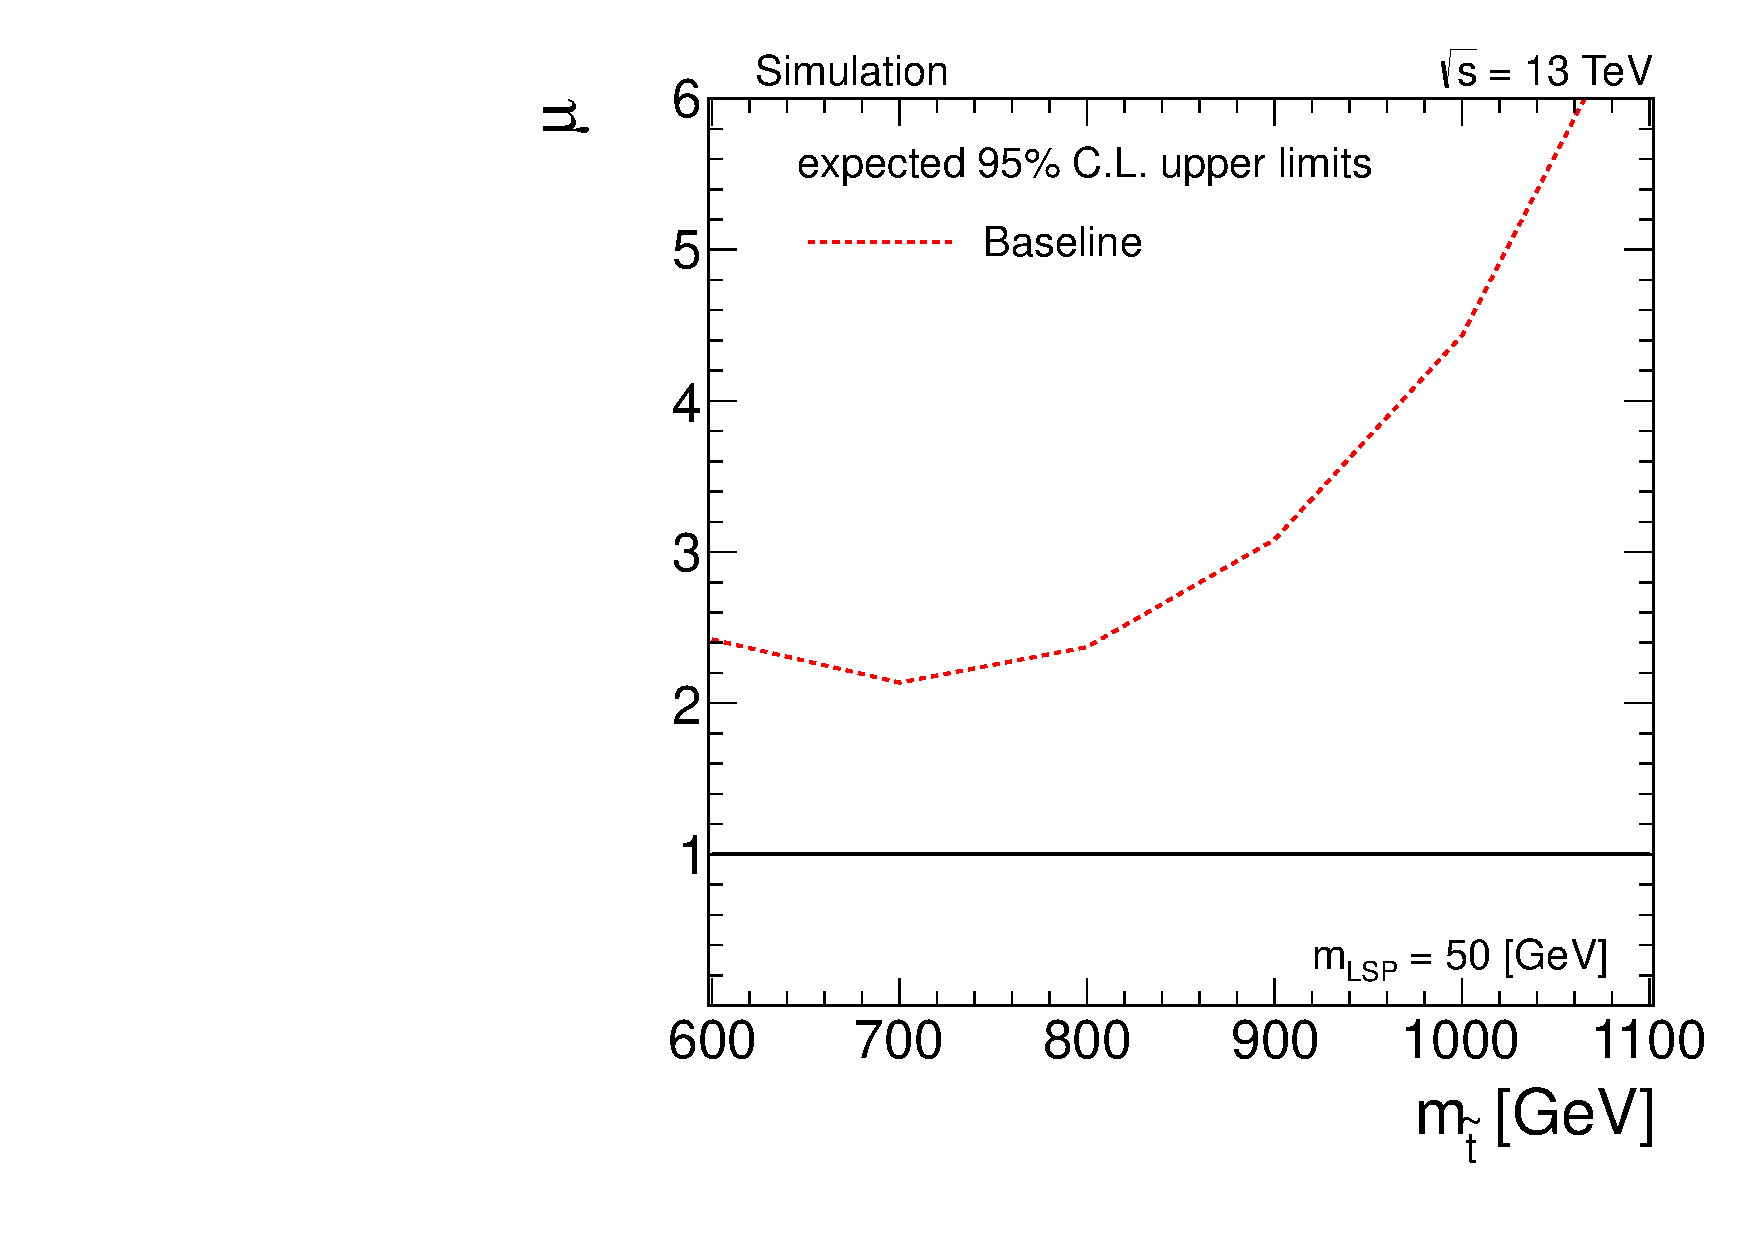
\includegraphics[width=0.49\textwidth]{figures/limitplot4BinSel_Baseline_LSP50.pdf} 
  \end{tabular}
  \caption{Expected 95\% upper limit for signal strength versus $m_{\tilde{t}}$. The LSP mass is chosen to be 50\gev.}
  \label{fig:stop_baseline_limit}
\end{figure}

\section{Sensitivity Improvement using B Tagging}
\label{sec:stop_btagging}
As illustrated in Fig.~\ref{fig:T2tt}, the targeted signal final state involves the presence of bottom quarks emerging from the decay of the top quarks. Thus, an obvious option to enhance the sensitivity of such an analysis is to employ b-tagging techniques to identify b quarks in the final state. Typical b-tagging algorithms for the identification of b-quark jets used within the CMS experiment have been discussed in Section~\ref{sec:btagging}. \\
In this analysis, b-quark jets are identified based on the CSV algorithm using the medium working point. Furthermore, they are required to have \pt$> 30$\gev in order to be not sensitive to potentially large flavour-dependent JEC uncertainties for jet transverse momenta smaller than 30\gev. In Fig.~\ref{fig:stop_baseline_btag}, the b-tag multiplicity, \ie the number of b-tagged jets in the event, is illustrated.  %As expected the maximum of this distribution for signal and \ttbar events is around two, since two b-quark jets are expected from the two decaying top quarks. \\ %Values above two or b-tagged jets in backgrounds not containing real b-quarks can be explained by the misidentification rate of the tagging algorithm. \\ 
When imposing in addition to the baseline selection also a requirement of at least one b-tagged jet, the total signal efficiencies for the signal samples with stop masses of 600\gev and 1100\gev decrease from around 30\% and 48\% to 25\% and 38\%, respectively. However, also the total background efficiency decreases significantly from $1.2 \cdot 10^{-7}$ to $3.6 \cdot 10^{-8}$. Concerning background events, the main reduction occurs for \WJets, \ZJets and QCD events as these contain in most cases no b-tagged jet. The relative background composition after applying the b-tag requirement is: 77.5\% \ttbar, 8.8\% \WJets, 8.6\% \ZJets and 5.1\% QCD.        
\begin{figure}[!t]
  \centering
  \begin{tabular}{c}
                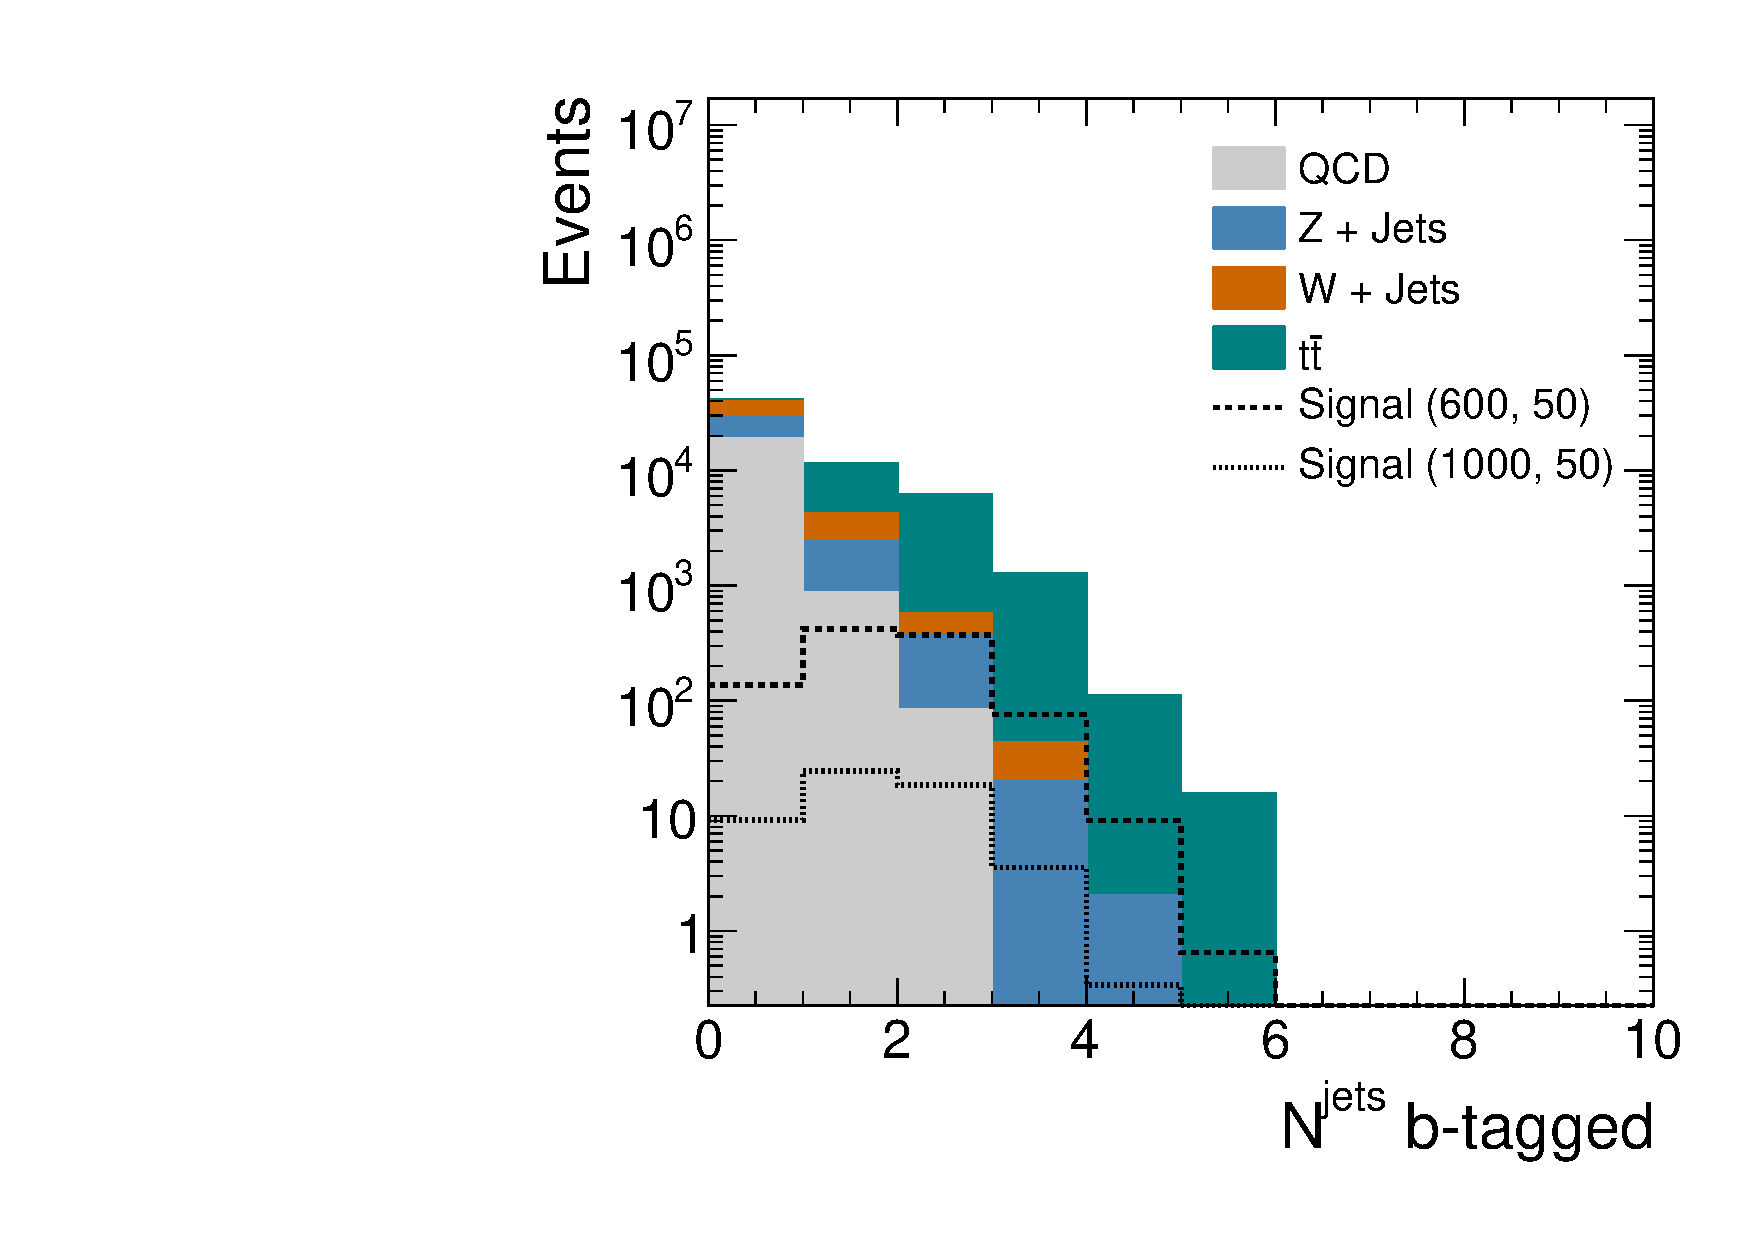
\includegraphics[width=0.49\textwidth]{figures/Stop_DeltaPhiSelection_N_jets_btagged.pdf}% &
       %         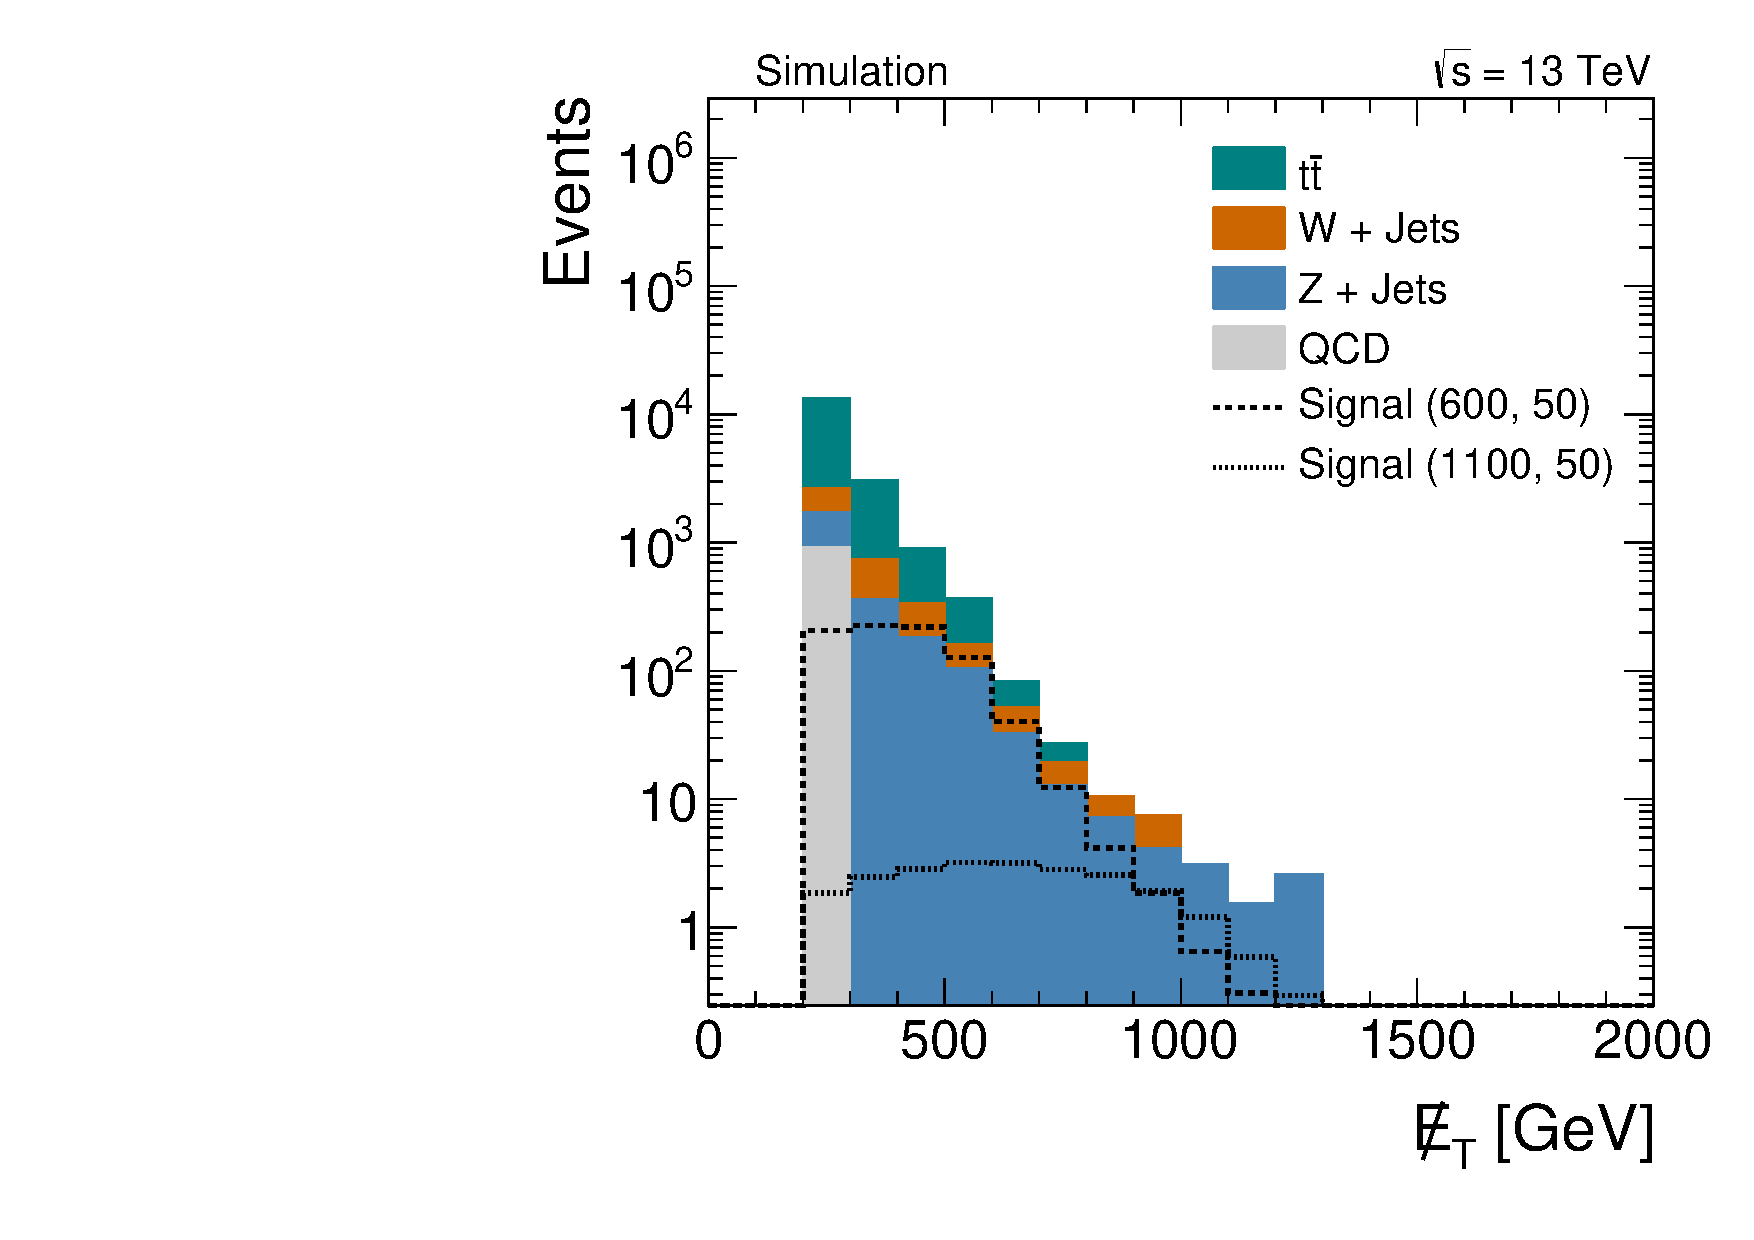
\includegraphics[width=0.49\textwidth]{figures/Stop_BTag_MET.pdf}   
  \end{tabular}
  \caption{B-tag multiplicity after applying the baseline selection in simulated events. The signal points are labelled as (X, Y) where X is the stop quark mass and Y is the LSP mass in GeV.}
  \label{fig:stop_baseline_btag}
\end{figure}
\\
Due to the improved signal to background ratios, also the expected exclusion limit of the analysis is expected to improve when applying the b-tag requirement in addition to the baseline selection. The same exclusive search regions as defined in Tab.~\ref{tab:stop_excl_search_bins} are used considering the same total uncertainties as described in Sec.~\ref{sec:stop_baseline} for a performance comparison of this improved selection with respect to the baseline requirements. The expected limit for the baseline selection including the additional b-tag requirement is shown in Fig~\ref{fig:stop_baselinebtag_limit}. 
\begin{figure}[!h]
  \centering
  \begin{tabular}{c}
                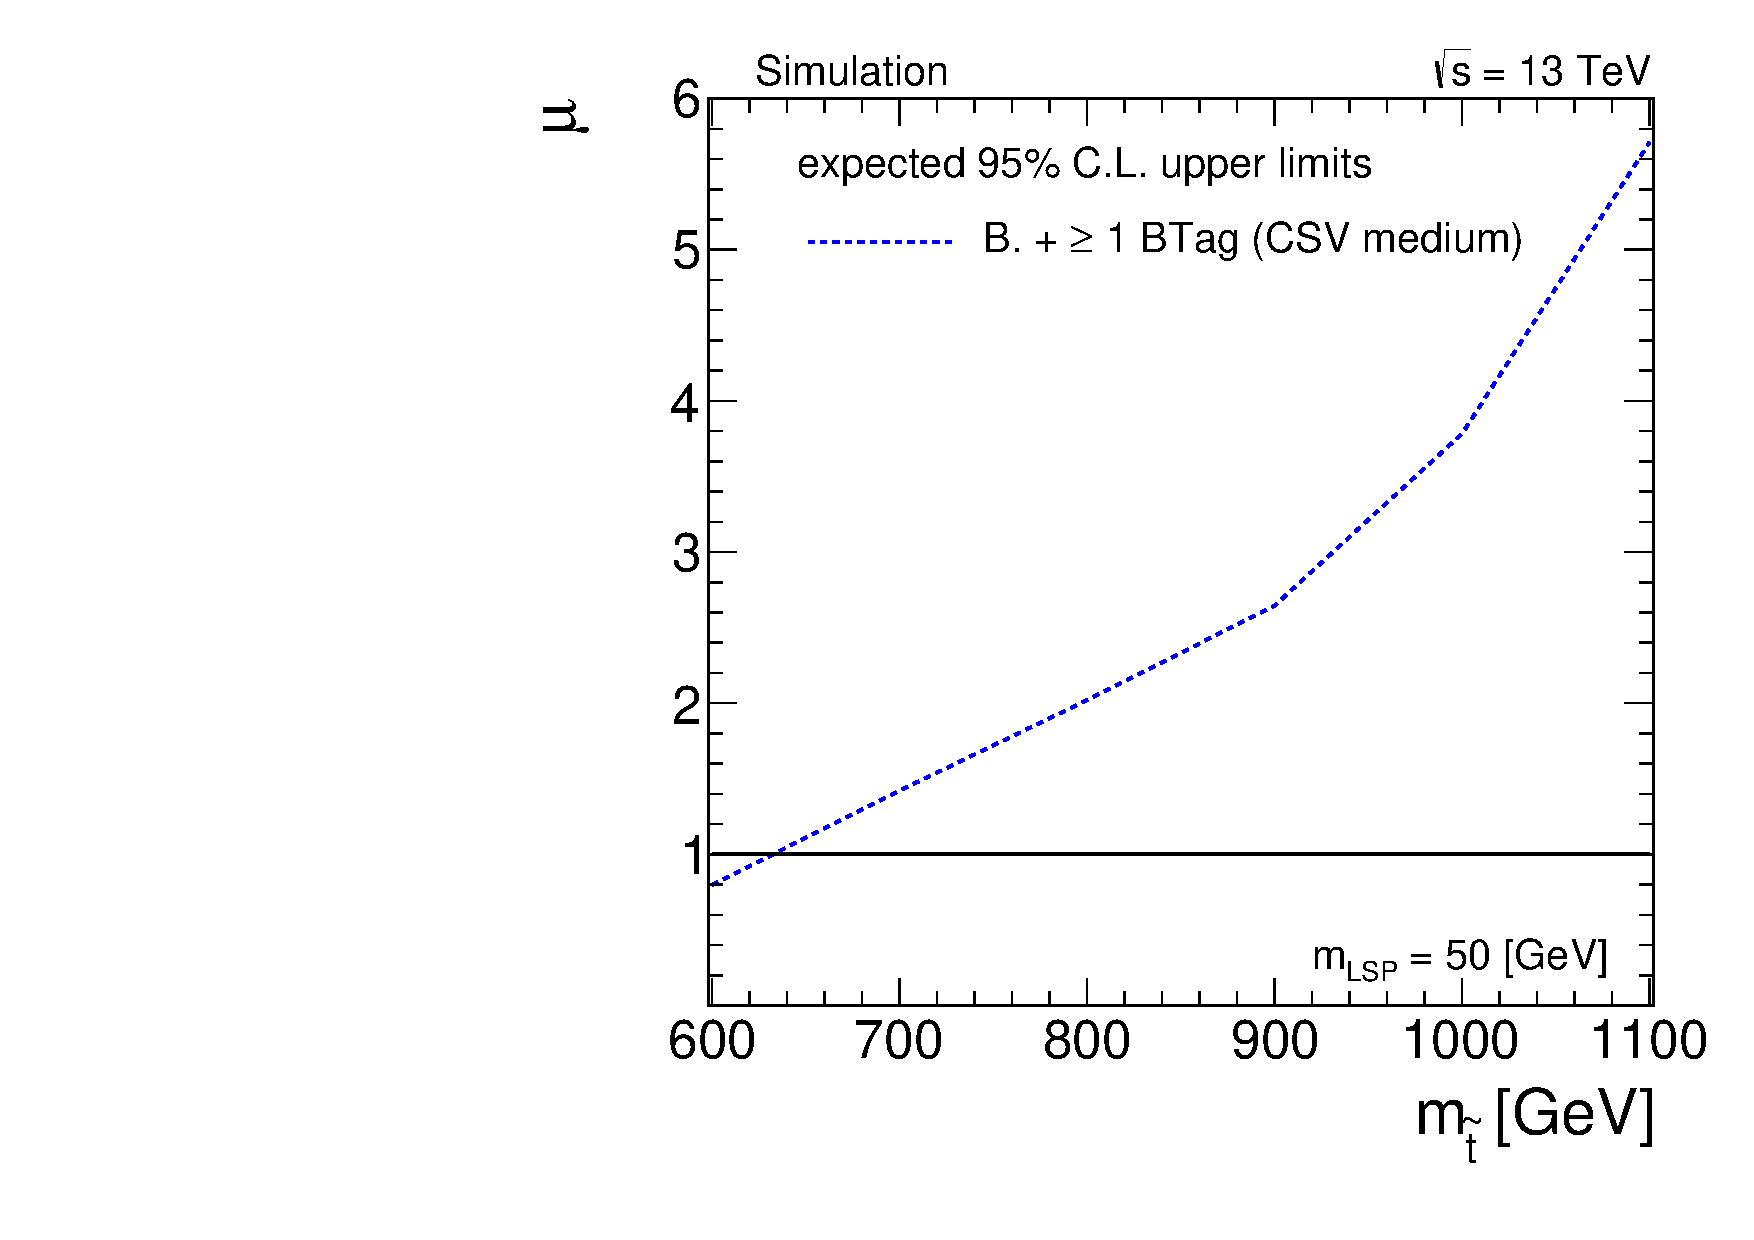
\includegraphics[width=0.49\textwidth]{figures/limitplot4BinSel_BaselineBTag_LSP50.pdf} 
  \end{tabular}
  \caption{Expected 95\% upper limit for signal strength versus $m_{\tilde{t}}$. The LSP mass is chosen to be 50\gev. The label B. denotes the baseline selection.}
  \label{fig:stop_baselinebtag_limit}
\end{figure}
\\
It turns out that the b-tag requirement significantly improves the sensitivity of the analysis towards the whole specified stop quark mass range and $\mu$ drops below one for lower masses so that these can be probed with such an analysis strategy. However, since the focus of this analysis is put on higher stop quark masses, it is discussed in the next section how this mass range can be adressed better.  

\section{Sensitivity Improvement using Top Tagging}
\label{sec:stop_toptagging}
\begin{figure}[!t]
  \centering
  \begin{tabular}{c}
                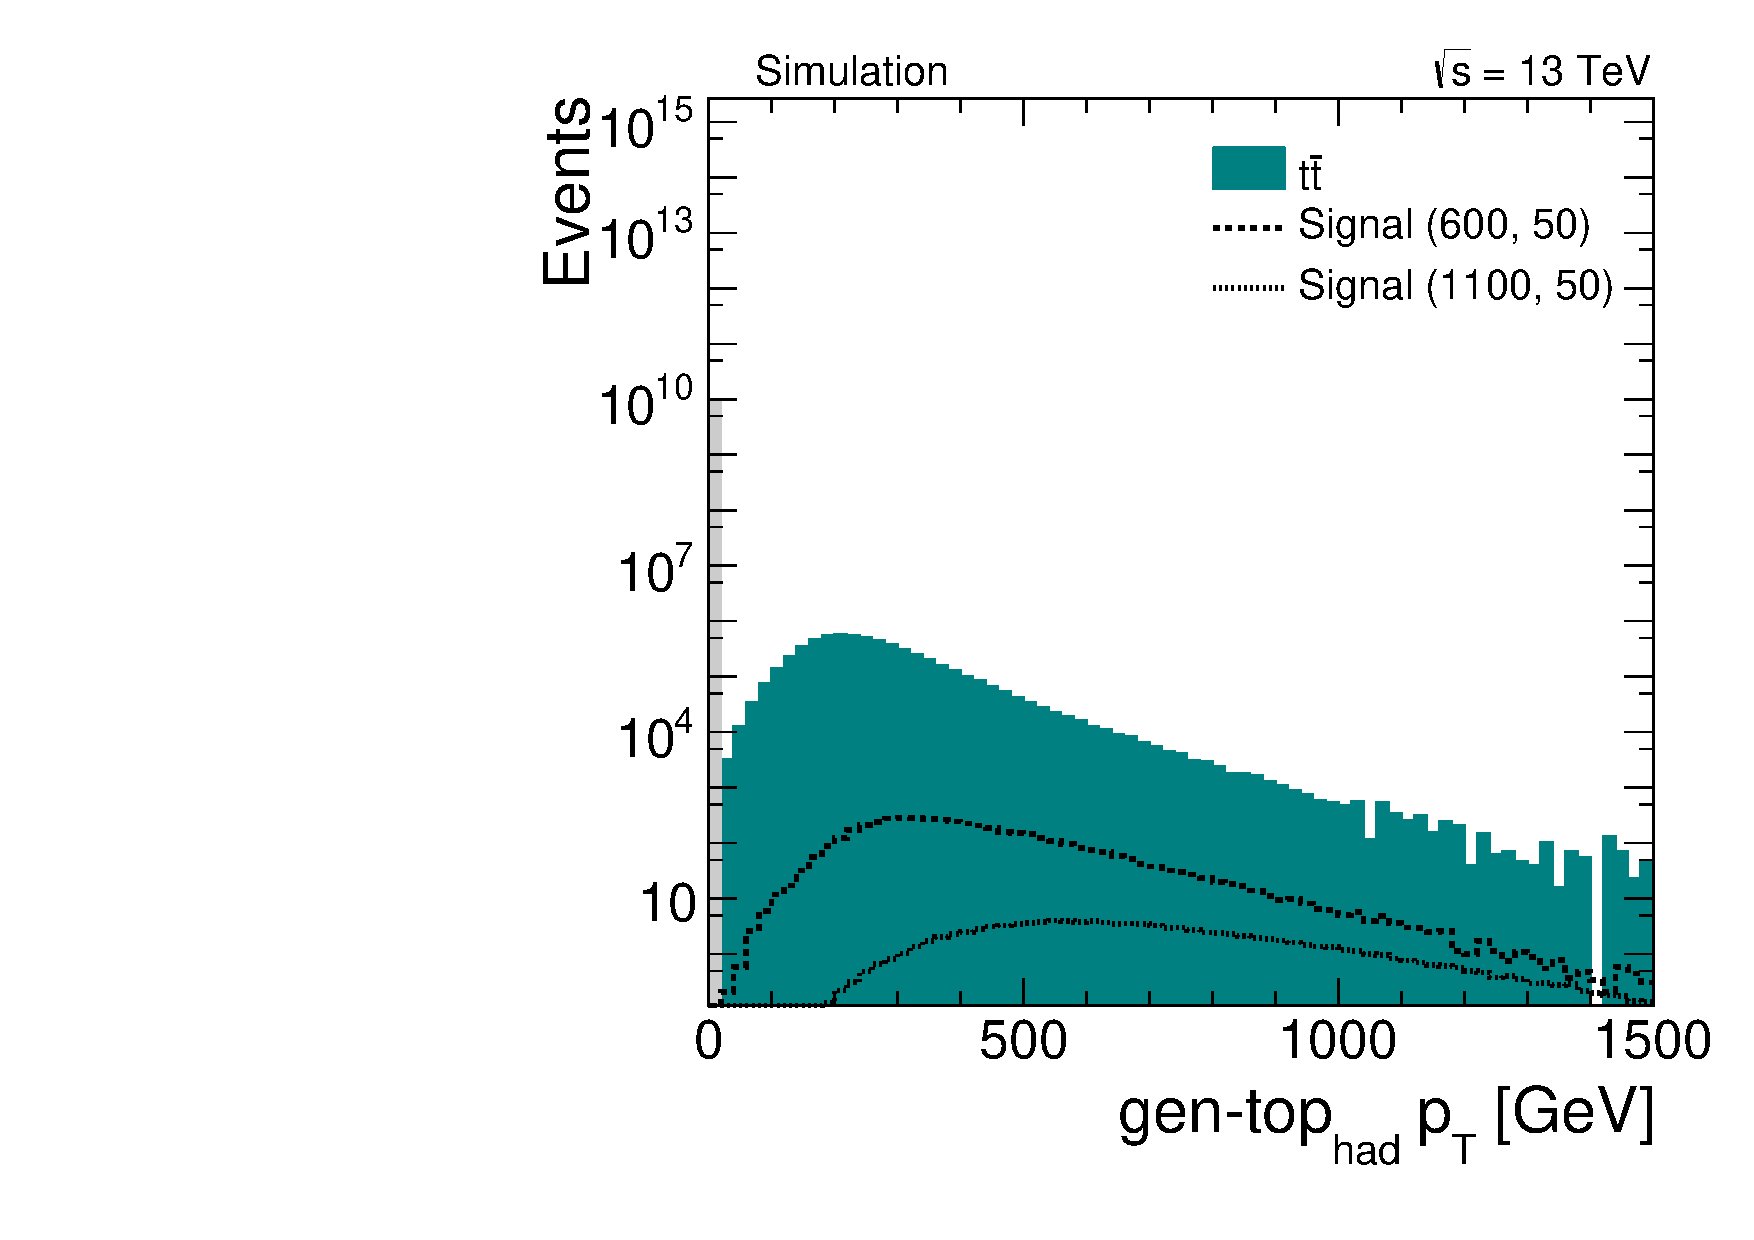
\includegraphics[width=0.49\textwidth]{figures/Stop_NoCuts_leading_had_t_ptgen.pdf} 
  \end{tabular}
  \caption{Transverse momentum spectrum of the leading generated hadronically decaying top quarks without applying any selection criteria. The signal points are labelled as (X, Y) where X is the stop quark mass and Y is the LSP mass in GeV.}
  \label{fig:stop_gen_top_pt}
\end{figure} 
In order to gain a better understanding of the kinematics of the investigated final state, the \pt spectrum of the leading generated  hadronically decaying top quark is illustrated in Fig.~\ref{fig:stop_gen_top_pt} for \ttbar background and two selected signal points without applying any selection criteria. As expected, the \pt spectrum of the signal is significantly harder than that of the \ttbar background. For instance for a stop mass of 1100\gev the maximum lies at a \pt range around 400--500\gev. As discussed in Sec.~\ref{sec:boosted_tops}, decay products emerging from the decay of a top quark with large transverse momentum can be reconstructed as a single jet with large radius parameter. Following Eq.~\ref{eq:rule-of-thumb}, the opening angle of decay products from a top quark with transverse momentum between 400--500\gev is expected to be $R = 0.8$. Thus, such topologies are well suited to utilize the top tagging techniques described in Sec.~\ref{sec:boosted_tops}. \\
The performance of the CMS- and the HEP-top-tagging algorithms are investigated based on the 13\tev simulation samples and reviewed in the following. 
\begin{description}
\item {\textbf{Top-Tagging Efficiency Studies:}} In order to evaluate the performance of the top-tagging algorithms, the top-tagging efficiencies and misidentification rates are derived. While the top-tagging efficiency is determined for \ttbar events, the QCD multijet sample is used to measure the misidentification rate. \\
The top-tagging efficiency is defined as the number of hadronically decaying generated top quarks matched to a top-tagged CA-jet divided by the number of all generated hadronically decaying generated top quarks. A successful match is identified by requiring the $\Delta R$ of a generated top quark and a top-tagged CA-jet to be less than the jet radius parameter which is $R=0.8$ for the CMS top tagger and $R=1.5$ for the HEP top tagger, respectively. The obtained efficiencies as a function of the transverse momentum of the generated hadronically decaying top quark are shown in the left part of Fig.~\ref{fig:stop_top_eff} for both the CMS and the HEP top tagger. It is visible that the turn-on of the HEP top tagger starts already around a \pt of 200\gev while the CMS tagger begins to become efficient not before around a \pt of 400\gev. However, the efficiency of the HEP top tagger lies around 20\% in the plateau region while the plateau efficiency of the CMS top tagger is in general higher with a value of around 25\%. This behaviour results mainly from the different jet sizes and selection criteria which are in case of the HEP top tagger optimized to be sensitive already in the \pt range around 200--300\gev.
\begin{figure}[!t]
  \centering
\makebox[\linewidth]{
  \begin{tabular}{cc}
                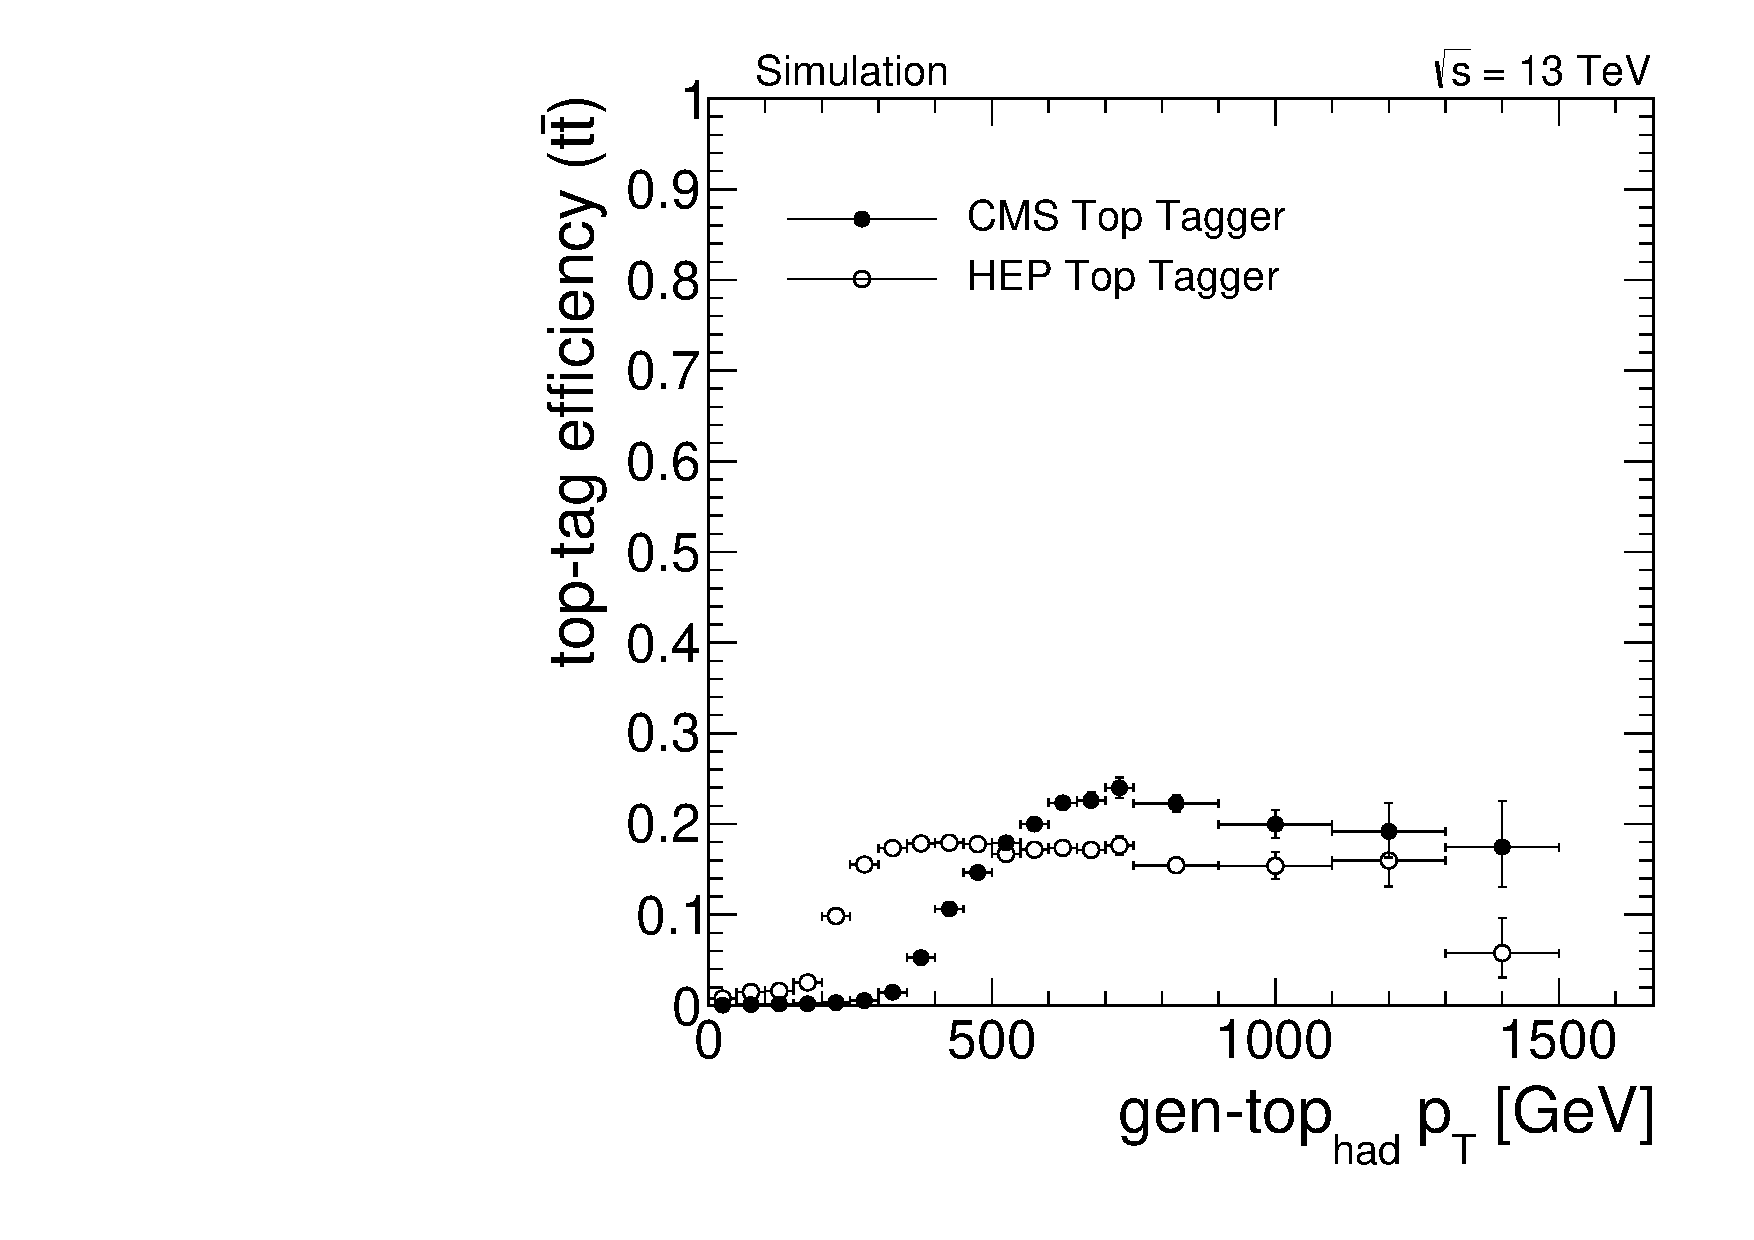
\includegraphics[width=0.49\textwidth]{figures/Comparison_TopTagEfficiencyGenTopPt_13TeV.pdf} & 
                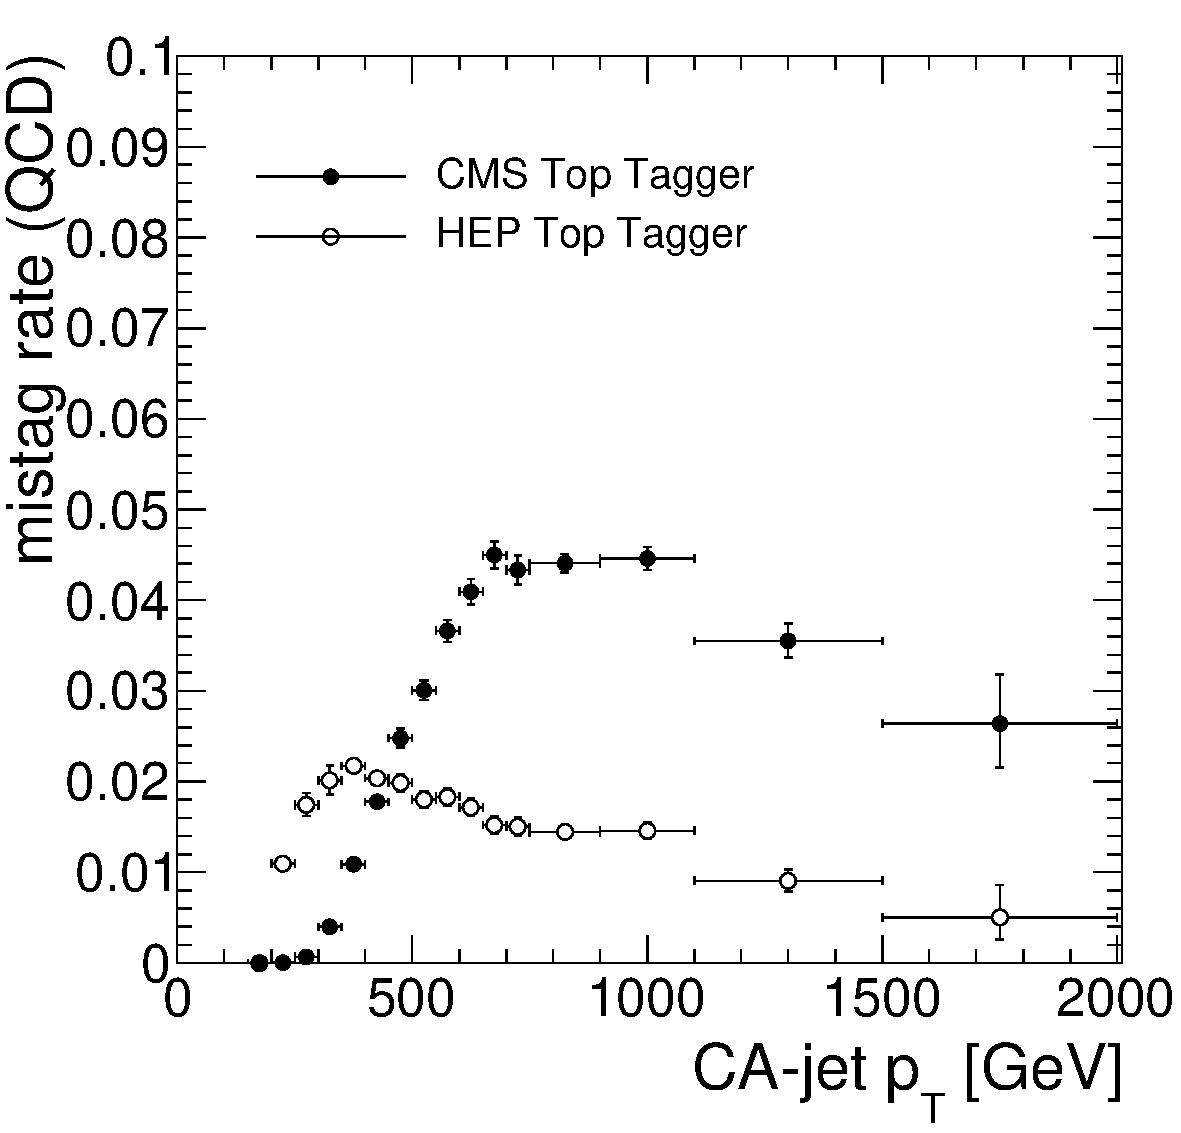
\includegraphics[width=0.49\textwidth]{figures/Comparison_MistagRate_13TeV.pdf} \\
  \end{tabular}}
  \caption{Top-tagging efficiency for \ttbar events as function of the transverse momentum of the generated hadronically decaying top quark (\textit{left}) and misidentification rate for QCD multijet events as a function of the CA-jet \pt (\textit{right}). In case of the CMS top tagger CA-jets with a distance parameter of $R=0.8$ are used while the HEP top tagger is based on CA-jets with $R=1.5$.}
  \label{fig:stop_top_eff}
\end{figure} 
\\
The misidentification rate can be evaluated by dividing the number of top-tagged CA-jets by the number of all CA-jets. The misidentification rate as a function of the respective CA-jet transverse momentum is shown in the right part of Fig.~\ref{fig:stop_top_eff}. Here, a similar feature as for the efficiency curve is observed. The HEP top tagger shows a certain misidentification rate already for lower transverse momenta than the CMS top tagger. However, in general the misidentification rate of the HEP top tagger is significantly smaller with a plateau around 1.5\% compared to the CMS top tagger which shows a misidentification rate of up to 4--5\% in the plateau. \\
Often, in analyses based on top quarks with moderate transverse momenta, that suffer mainly from QCD background, the HEP top tagger is a good choice, since the efficiency has an early turn-on and the misidentification rate is small. However, if the main background contains actual top quarks, as it is the case for stop quarks, the more important property is an efficiency as high as possible to retain signal efficiency while the misidentification rate only plays a less important role. 
\end{description}
\begin{figure}[!t]
  \centering
\makebox[\linewidth]{
  \begin{tabular}{cc}
                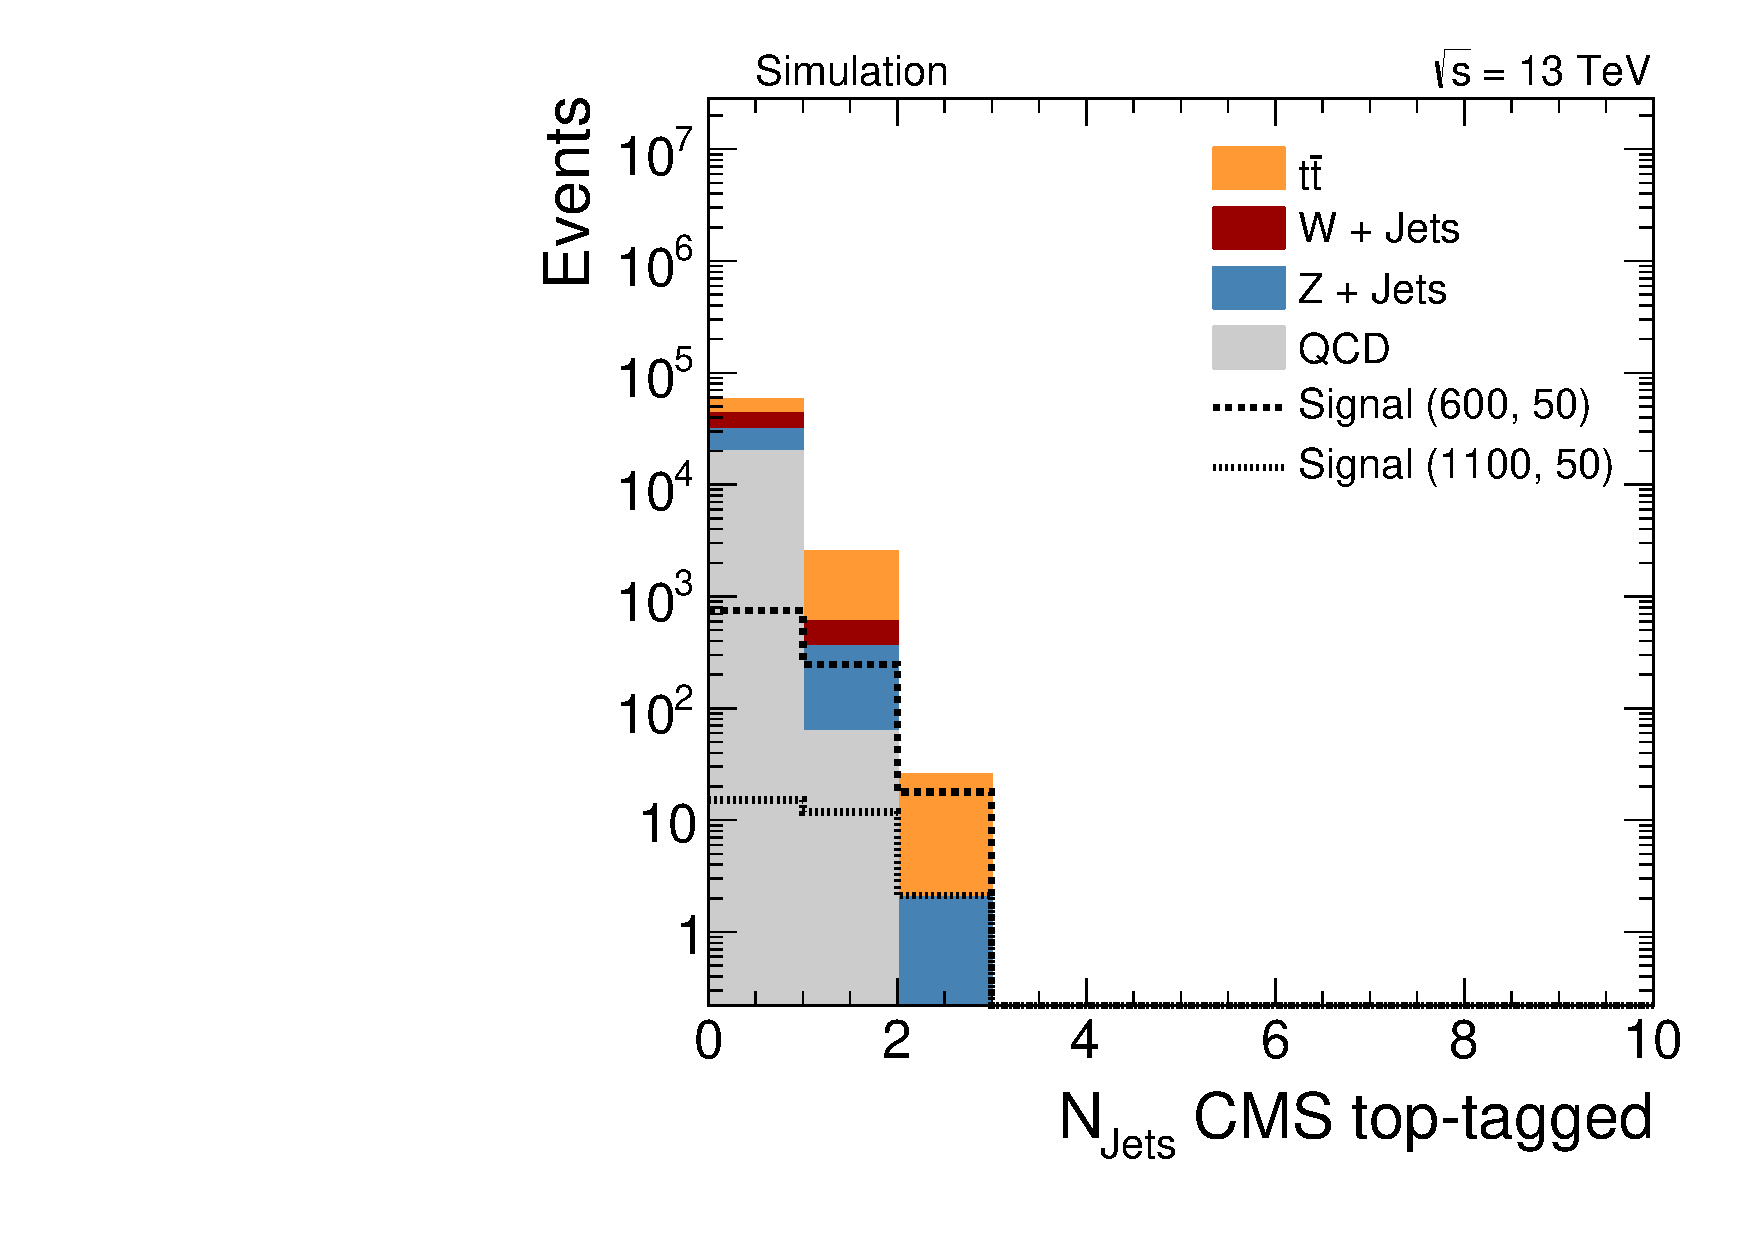
\includegraphics[width=0.49\textwidth]{figures/Stop_DeltaPhiSelection_N_jets_toptagged.pdf} & 
                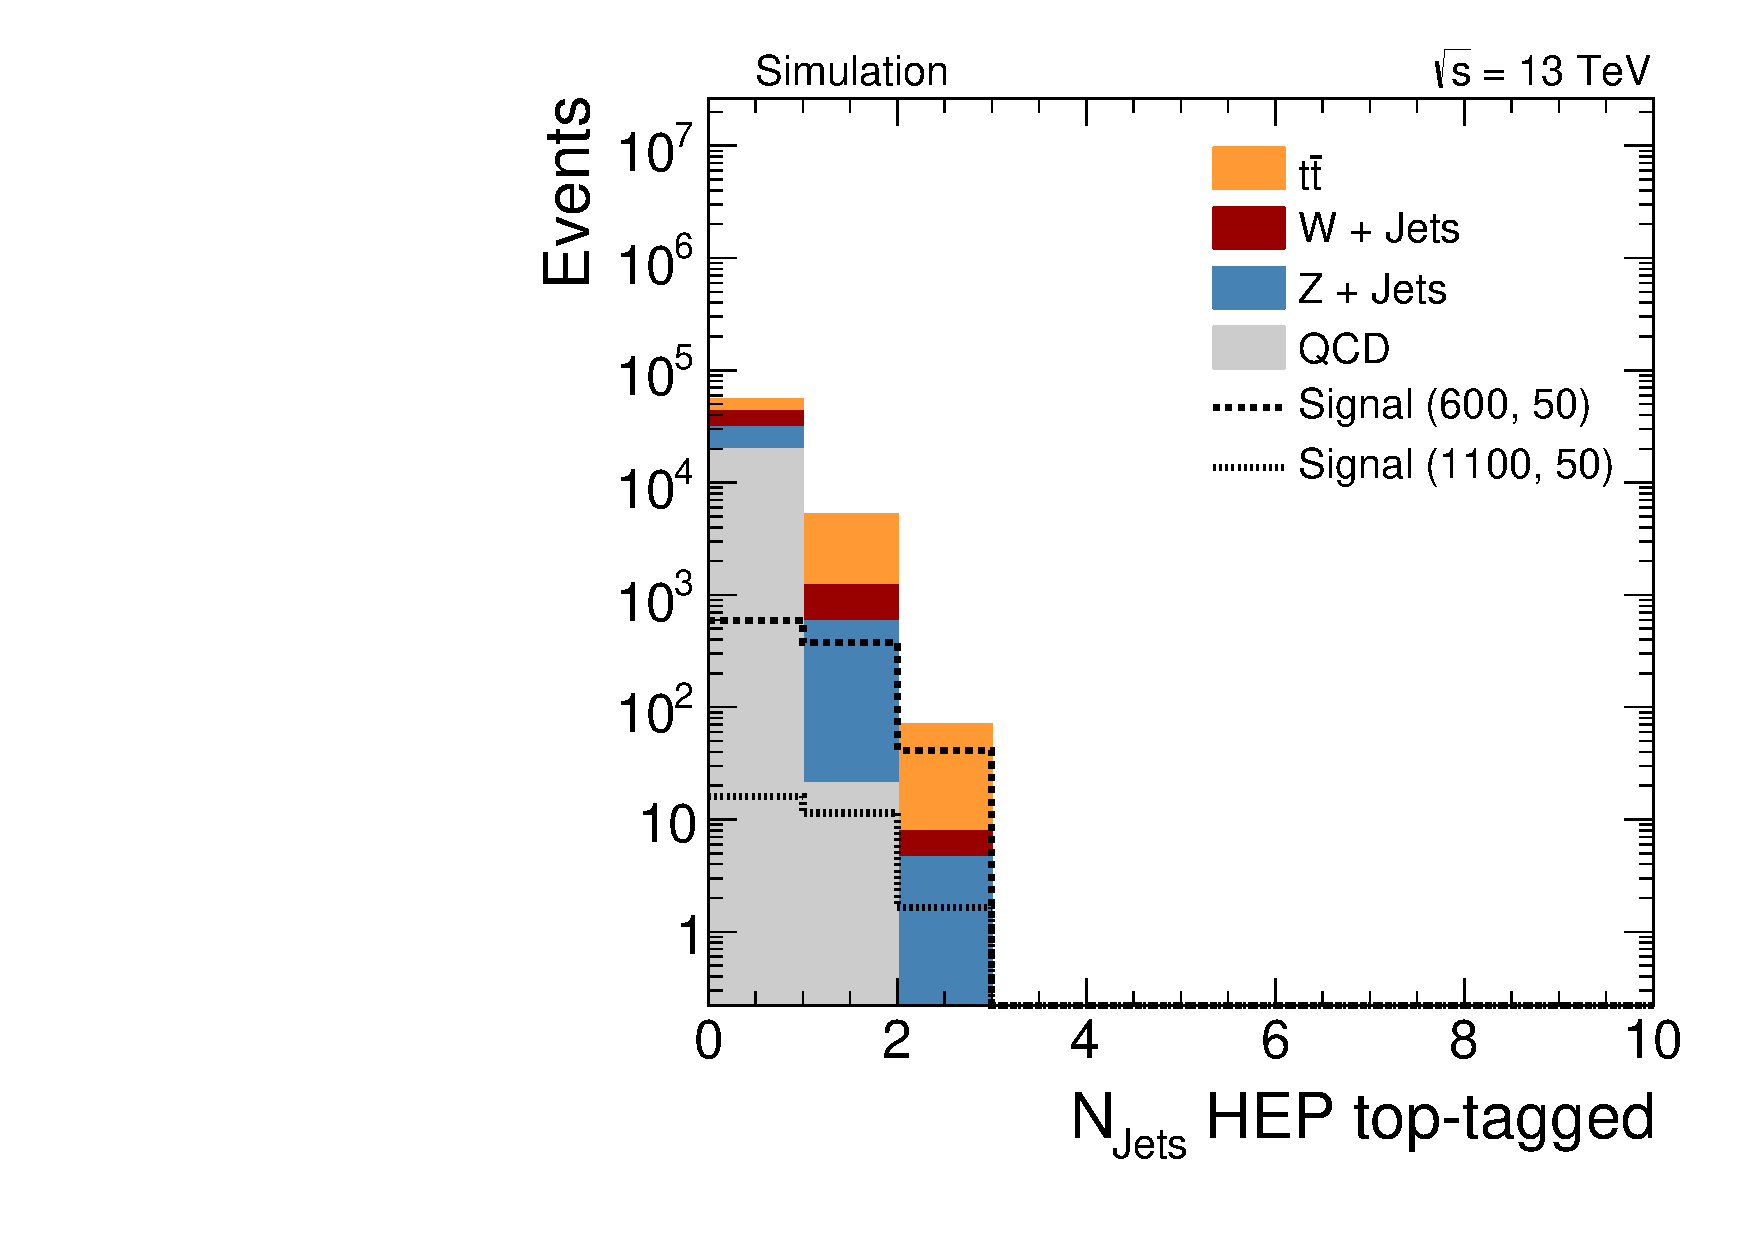
\includegraphics[width=0.49\textwidth]{figures/Stop_DeltaPhiSelection_N_jets_HEPtoptagged.pdf} \\
  \end{tabular}}
  \caption{Top-tag multiplicity for the CMS top tagger (\textit{left}) and the HEP top tagger (\textit{right}) after application of the baseline selection. Only CA-jets of the corresponding jet size with a transverse momentum above 150\gev are considered.}
  \label{fig:stop_top_tag_multi}
\end{figure} 
The impact on the analysis when applying top tag requirements can be studied when looking for instance at the top tag multiplicity. In Fig.~\ref{fig:stop_top_tag_multi}, the top tag multiplicity is shown for the CMS top tagger (left) and the HEP top tagger (right) after the application of the baseline selection. Here, only CA-jets of the corresponding jet size with a transverse momentum above 150\gev are considered, since the taggers are not supposed to be efficient for smaller momenta. \\
Although a significant amount of signal events does not have a CA-jet identified as top-jet by the respective algorithm, the distributions exhibit that the background can be significantly reduced when requiring at least one top-tagged jet. The respective signal and background efficiencies, when using in addition to the baseline selection a requirement of at least one top-tagged jet, evolve as follows when considering the total efficiencies not separated according to the individual search regions:
\begin{itemize}
 \item HEP top tagger: \\
$\epsilon_\mathrm{sig}^\mathrm{m_{\tilde{t}} = 600\gev}$ = 12\%, $\epsilon_\mathrm{sig}^\mathrm{m_{\tilde{t}} = 1100\gev}$ = 22\% \\
$\epsilon_\mathrm{bg}^\mathrm{total}$ = $1.1 \cdot 10^{-6}$\% , $\epsilon_\mathrm{bg}^\mathrm{\ttbar}$ = 0.03\% 
 \item CMS top tagger: \\
$\epsilon_\mathrm{sig}^\mathrm{m_{\tilde{t}} = 600\gev}$ = 8\%, $\epsilon_\mathrm{sig}^\mathrm{m_{\tilde{t}} = 1100\gev}$ = 23\% \\
$\epsilon_\mathrm{bg}^\mathrm{total}$ = $0.5 \cdot 10^{-6}$\% , $\epsilon_\mathrm{bg}^\mathrm{\ttbar}$ = 0.01\% 
\end{itemize}
In general, the signal efficiency for low masses is larger when using the HEP top tagger than for the CMS top tagger and comparable for the higher stop mass. However, also the background efficiency shows a larger value for the HEP top tagger case and in particular more \ttbar events are selected. Thus, the CMS top tagger is expected to provide a better search sensitivity. \\
In order to test the impact of the top tagging requirements on the search sensitivity more quantitatively, the expected limits are derived again based on the search regions defined in Tab.~\ref{tab:stop_excl_search_bins} with the same uncertainties as assumed in Sec.~\ref{sec:stop_baseline}. The results are illustrated in Fig~\ref{fig:stop_baselinetoptag_limit}. As expected, for the HEP top tagger as well as for the CMS top tagger the usage of a top tag requirement in addition to the baseline selections significantly improves the search sensitivity. The improvement amounts to a factor of two to three. Hence, mass points up to ($m_{\tilde{t}}, m_\mathrm{LSP}$) = (700, 50)\gev or even (800, 50)\gev can be probed with such selections. This selection is also more sensitive than the result obtained when adding a b-tag requirement as discussed in Sec.~\ref{sec:stop_btagging} which allows to probe stop masses around 600\gev for an LSP mass of 50\gev. In general, the selection based on the CMS top tagger performs better than the selection involving the HEP top tagger, since the signal to background ratio is higher as discussed above. 
\begin{figure}[!t]
  \centering
  \begin{tabular}{c}
                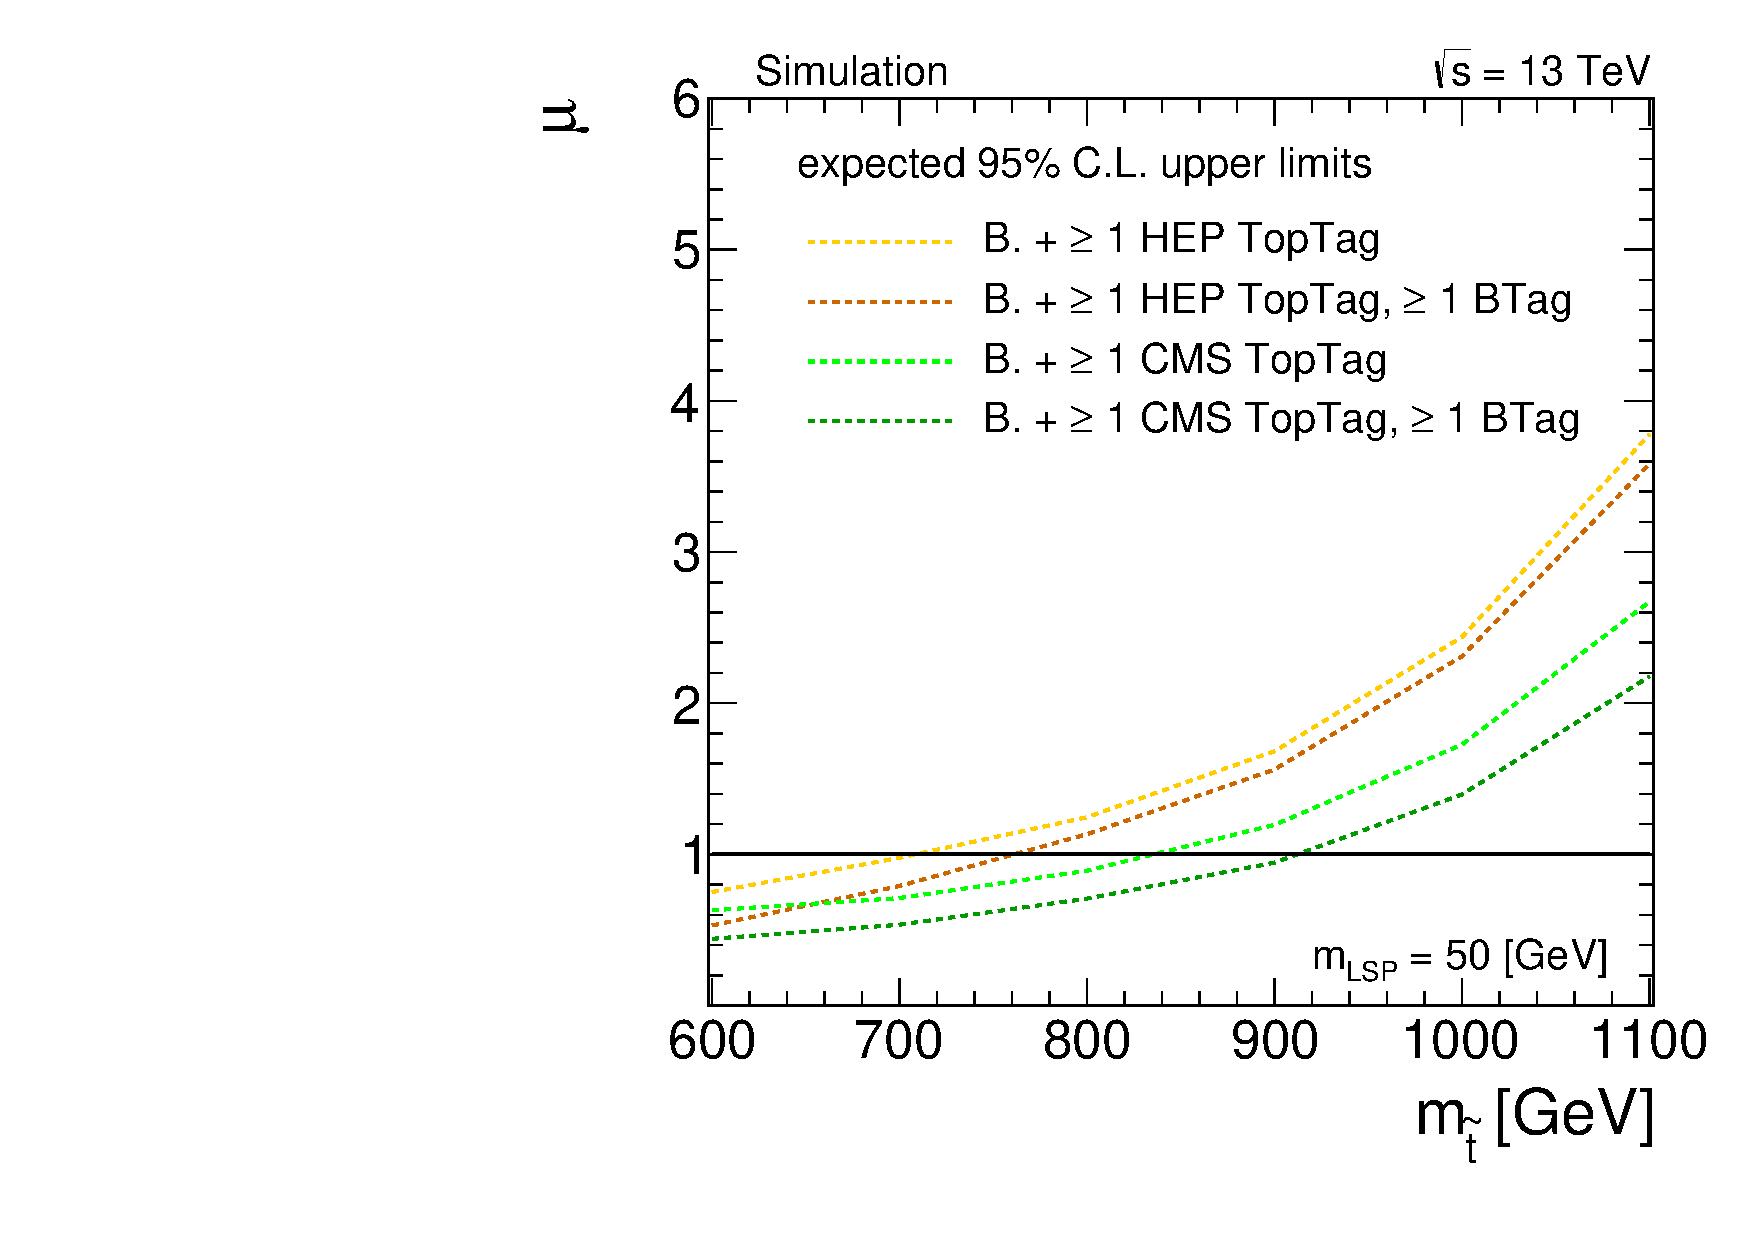
\includegraphics[width=0.49\textwidth]{figures/limitplot4BinSel_BaselineBTagTopTag_LSP50.pdf} 
  \end{tabular}
  \caption{Expected 95\% upper limit for signal strength versus $m_{\tilde{t}}$. The LSP mass is chosen to be 50\gev. The label B. denotes the baseline selection.}
  \label{fig:stop_baselinetoptag_limit}
\end{figure}
\\
Furthermore, the selections including the top tagging requirements are also compared when imposing an additional b-tag requirement, as defined in Sec.~\ref{sec:stop_btagging}. In both cases the b-tag requirement further improves the sensitivity. The selection involving the CMS top tagger still performs better. Thus, selections utilizing the HEP top tagger are not pursued in the following.% After the requirement of at least one top-tagged jet, \ttbar is the largest background contribution (in total \todo{\%}). Thus, it is of particular interest to identify kinematic selections that are specifically suited to reduce the \ttbar background, as discussed in the following section.


\section{Performance Comparison of Various Kinematic Selections}
\label{sec:stop_cuts}
The sensitivity of the analysis targeting direct stop quark production using the baseline requirements discussed in Sec.~\ref{sec:stop_baseline} can be improved already significantly when employing in addition b-tag and top-tag requirements, as shown in Sec.~\ref{sec:stop_btagging} and~\ref{sec:stop_toptagging}. Nevertheless, the sensitivity might still be improved when imposing further kinematic selections. \\
In order to address the specific kinematics of the various background contributions, first the background composition is studied in more detail. In Fig.~\ref{fig:stop_top_channels}, the background and signal processes are shown according to the decay mode of the process after the application of the baseline selection (left) and the baseline selection with an additional requirement of $\ge 1$ CMS top tag (right). These channels are defined according to the top quark properties based on generator information. The first channel includes all non-top backgrounds and the all-hadronic top decays. Channels two to four are the semi-leptonic top decays which contain electrons (channel two), muons (channel three) and tau leptons (channel four). Dileptonic \ttbar events are not displayed, as these are found to be negligible. The distributions exhibit that after the application of the top-tagging requirement, similarly to the b-tag requirement, the main background contribution arises from \ttbar events (around 77\%). Here, contributions from lost-leptons (channel two and three) and hadronically decaying tau leptons (channel four) occur in about equal amounts with slightly more hadronic tau events. Since in general the number of events is small after application of the top tag requirement, kinematic selections and their performance are investigated when applying baseline selection criteria. Nonetheless, since \ttbar is known to be the largest background after top tagging, special emphasis is put on reducing the \ttbar background contributions.
\begin{figure}[!t]
\centering
\makebox[\linewidth]{
\begin{tabular}{cc}
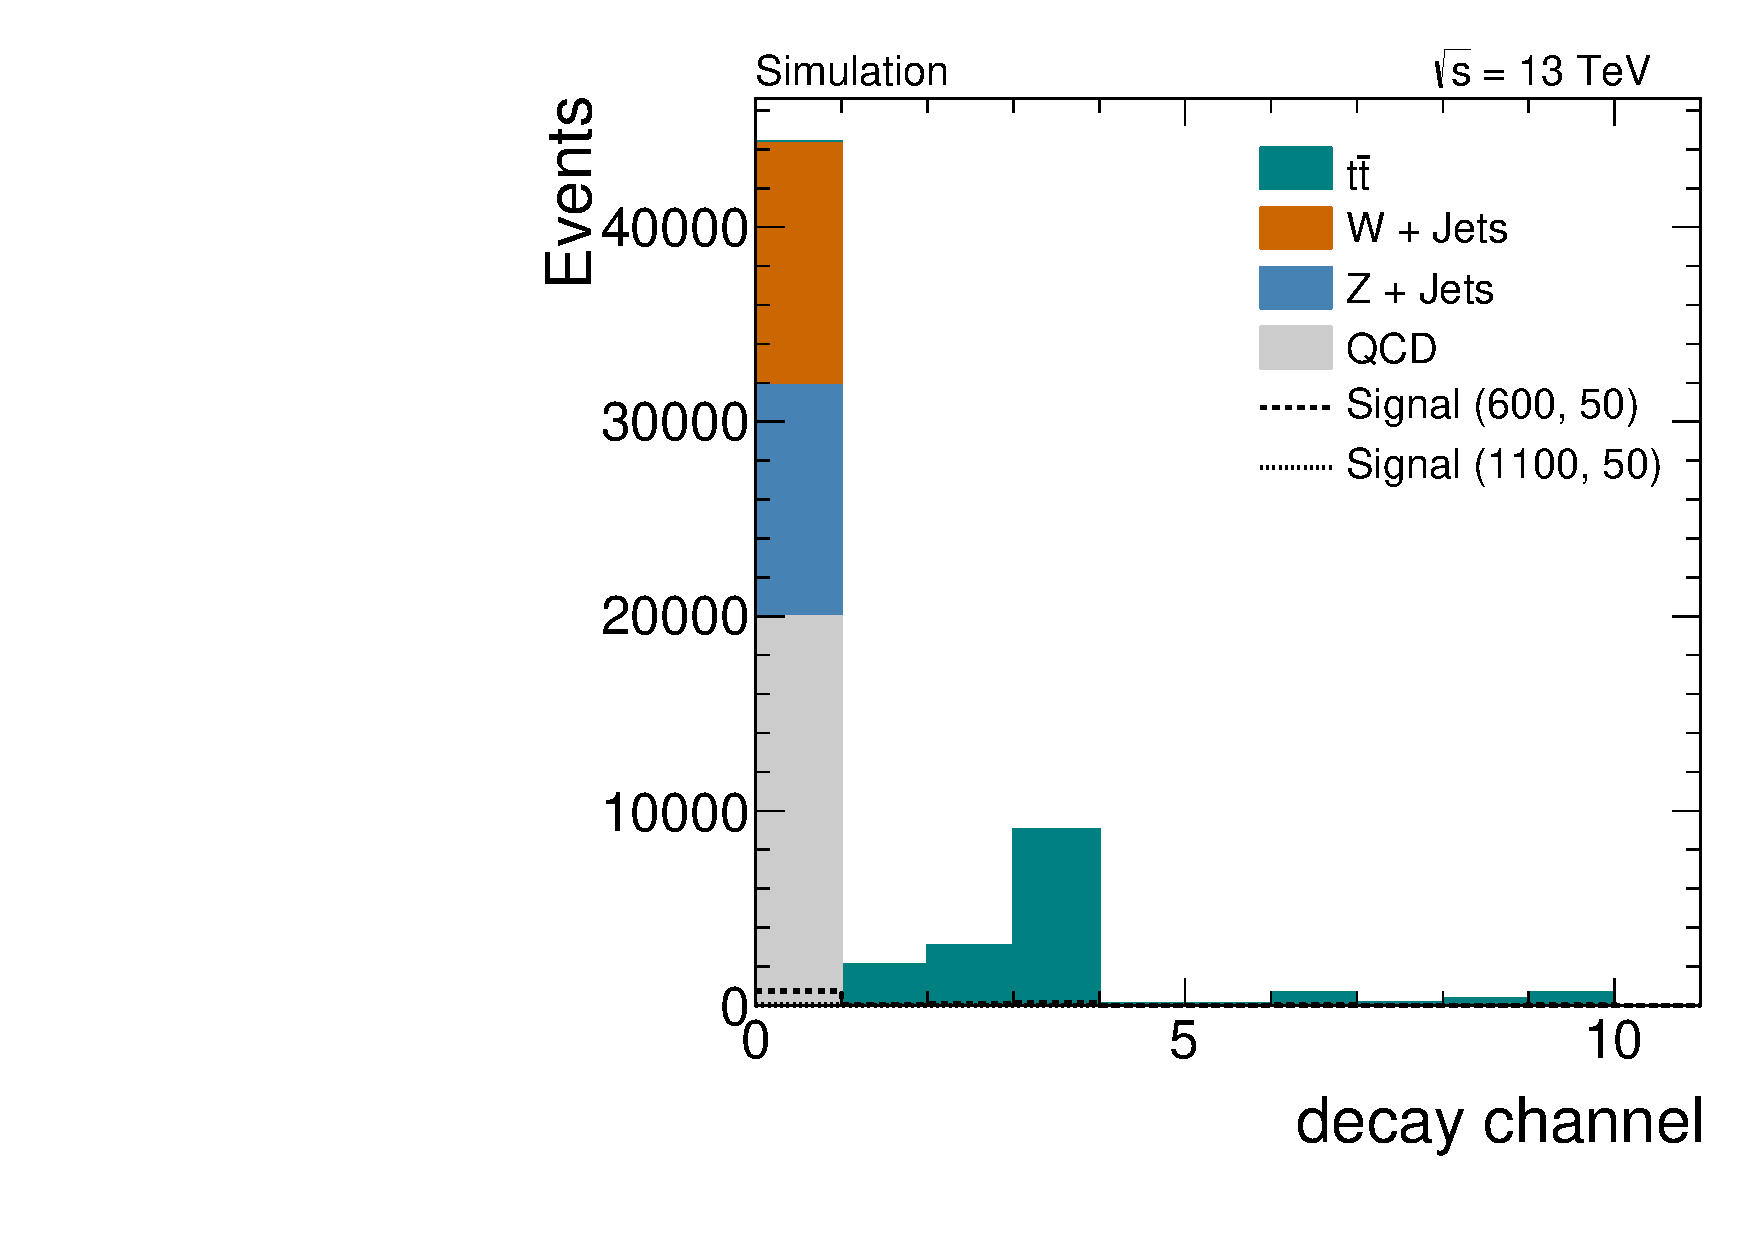
\includegraphics[width=0.49\textwidth]{figures/Stop_DeltaPhiSelection_t_decay_channels.pdf} &
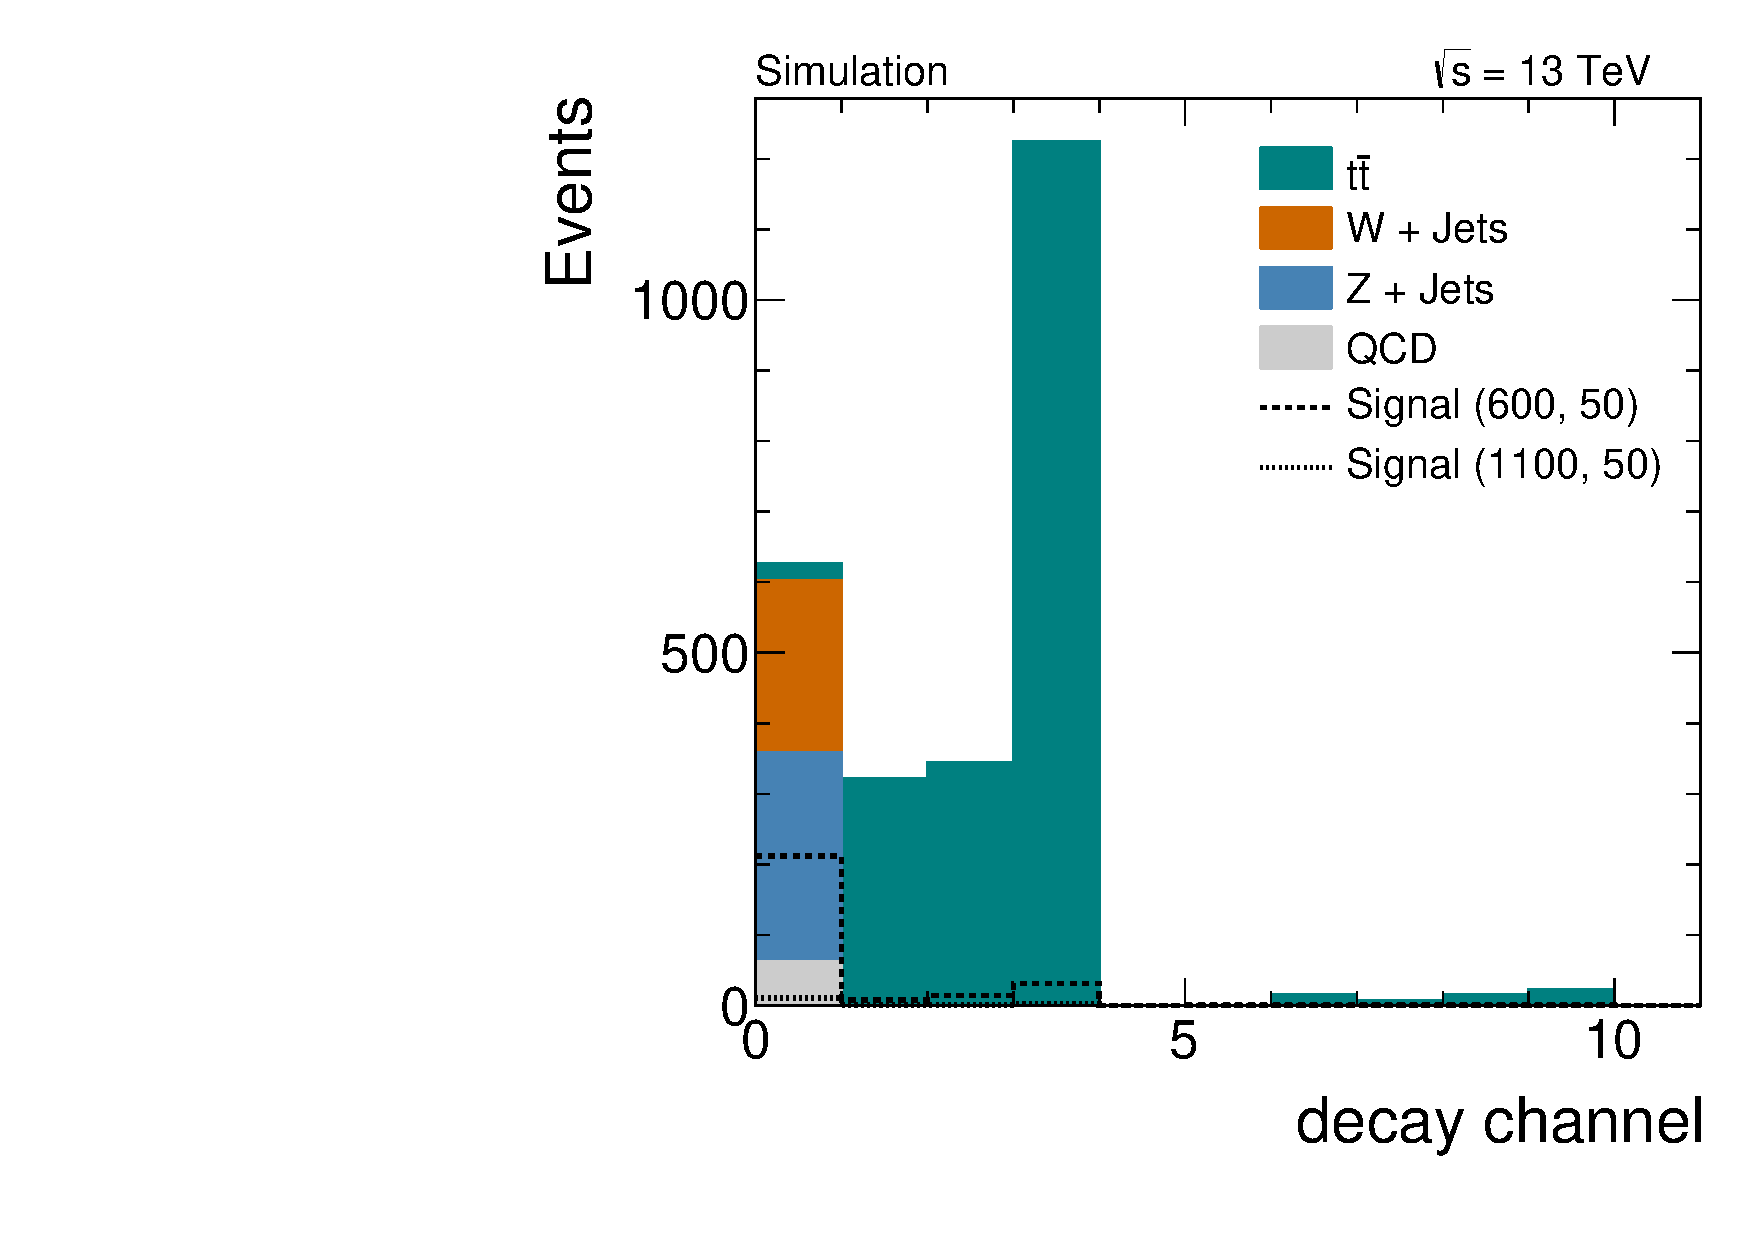
\includegraphics[width=0.49\textwidth]{figures/Stop_TopTag_t_decay_channels.pdf} \\
\end{tabular}}
\caption{Comparison of decay modes of signal and background processes defined according to the top quark properties based on generator information after the baseline selection (\textit{left}) and after the baseline selection and the requirement of $\ge 1$ CMS top tag (\textit{right}). For a definition of the decay channels see text.}
\label{fig:stop_top_channels}
\end{figure} 
\\
Several kinematic variables exist that have been successfully used already in various SUSY searches at $\sqrt{s} = 7$ and 8\tev:
\begin{description}
 \item $\mathbf{M_\mathrm{T2}:}$ The $M_\mathrm{T2}$ variable represents a generalized version of the transverse mass~\cite{Lester:1999tx, Barr:2003rg, Chatrchyan:2012jx, CMS-PAS-SUS-13-019}. In events with pair-produced particles which decay further and eventually contain undetectable particles in the decay products, \eg LSPs, the event kinematics are underconstrained and thus a classical transverse mass can not be determined. The $M_\mathrm{T2}$ variable is defined for two identical decay chains as
\begin{equation}
 M_\mathrm{T2}(m_{\tilde{\chi}}) = \min_{\vec{p}_\mathrm{T}^{\;\tilde{\chi}(1)} + \vec{p}_\mathrm{T}^{\;\tilde{\chi}(2)} = \vec{p}_\mathrm{T}^{\; \mathrm{miss}}} \left[ \mathrm{max} \left(M_\mathrm{T}^{(1)}, M_\mathrm{T}^{(2)} \right) \right] 
\end{equation} 
with the two transverse masses ($i = 1, 2$)
\begin{equation}
 (M_\mathrm{T}^{(i)})^2 = (m^{\mathrm{vis}(i)})^2 + m_{\tilde{\chi}}^2 + 2 \left( E_\mathrm{T}^{\mathrm{vis}(i)} E_\mathrm{T}^{\tilde{\chi}(i)} - \vec{p}_\mathrm{T}^{\; \mathrm{vis}(i)} \cdot \vec{p}_\mathrm{T}^{\; \tilde{\chi}(i)}   \right) 
\end{equation}
described by the transverse momenta $\vec{p}_\mathrm{T}^{\, \mathrm{vis}(i)}$, transverse energies $E_\mathrm{T}^{\mathrm{vis}(i)}$ and masses $m^{\mathrm{vis}(i)}$ for the visible systems and the unknown transverse momenta of the LSPs $\vec{p}_\mathrm{T}^{\tilde{\chi}(i)}$ with mass $m_{\tilde{\chi}}$. Experimentally, the momenta $\vec{p}_\mathrm{T}^{\tilde{\chi}(i)}$ are not accessible separately. Thus, a minimization on trial LSP masses fulfilling the constraint given by $\vec{p}_\mathrm{T}^{\; \mathrm{miss}}$, the missing transverse momentum,\footnote{More commonly denoted by \metvec in this thesis.} is performed. This minimization is carried out to make sure that $M_\mathrm{T2}$ does not exceed the mass of the parent particle. For the correct value of $m_{\tilde{\chi}}$, the distribution of $M_\mathrm{T2}$ is expected to have an endpoint at the mass of the parent particle. \\
In these studies, the two visible systems are assumed to be described by the two leading CA8 jets in the event and the mass of the neutralinos is considered to be zero. The calculation of $M_\mathrm{T2}$ is performed according to~\cite{Cheng:2008hk}. \\ 
The obtained distributions for $M_\mathrm{T2}$ in background and signal samples are shown in Fig~\ref{fig:stop_baseline_kin_vars} (top right). They exhibit that the maximum of $M_\mathrm{T2}$ is higher for signal events than for background such that this variable is suitable for distinguishing signal and background events.  
 \item \textbf{Razor variables:} The kinematic razor variables are used to describe the generic process of pair production of two heavy particles which subsequently decay into visible products usually represented by (large) jets and undetected particles~\cite{Chatrchyan:2012uea, Chatrchyan:2014goa, CMS-PAS-SUS-14-011}. These variables are used to test if the two jets represent the visible part of the decay of two heavy objects. \\
The razor variables are defined as
\begin{equation}
M_\mathrm{R} = \sqrt{\left[(|\vec{p}^{\; j_1} | + |\vec{p}^{\; j_2} |)^2 - (p_z^{\; j_1}  + p_z^{\; j_2} )^2 \right]}
\end{equation}
 \begin{equation}
M_\mathrm{T}^\mathrm{R} = \sqrt{\frac{1}{2} \left( \met (\pt^{\; j_1}  + \pt^{\; j_2} ) - \metvec \cdot (\vec{p}^{\; j_1} + \vec{p}^{\; j_2}) \right) }
\end{equation}
\begin{equation}
R = \frac{M_\mathrm{T}^\mathrm{R}}{M_\mathrm{R}}
\end{equation}
with the transverse momenta of the two jets $\pt^{j1}$ and $\pt^{j2}$. For signal events, $M_\mathrm{T}^\mathrm{R}$ has an endpoint and $R$ a maximum of approximately one. \\
For these studies, the two leading CA8 jets and \met are used to compute the razor variables. In Fig.~\ref{fig:stop_baseline_kin_vars} the variable $R^2$ is illustrated (bottom) after the application of baseline selection criteria. 
\item $\mathbf{\alpha_\mathrm{T}:}$ The $\alpha_\mathrm{T}$ variable is mainly used to reject QCD multijet events which have no intrinsic \met~\cite{Chatrchyan:2012wa, Chatrchyan:2013lya}. In case of dijet events, it is defined as:
\begin{equation}
 \alpha_\mathrm{T} = \frac{E_\mathrm{T}^{j_2}}{M_\mathrm{T}} \;\; \mathrm{and} \;\; M_\mathrm{T} = \sqrt{\left( \sum_{i=1}^{2} E_\mathrm{T}^{j_i} \right)^2 - \left( \sum_{i=1}^{2} p_\mathrm{x}^{j_i} \right)^2 - \left( \sum_{i=1}^{2} p_\mathrm{y}^{j_i} \right)^2}
\end{equation}
with the transverse energy $E_\mathrm{T}^{j_2}$ of the less energetic jet and the transverse mass $M_\mathrm{T}$ of the dijet system. Since in case of boosted top quark decays, the two top quarks are supposed to be represented each by one fat jet, the $\alpha_\mathrm{T}$ variable is in this studies calculated from the two leading CA8 jets. The distribution of the $\alpha_\mathrm{T}$ variable after application of the baseline selection requirements is shown in Fig.~\ref{fig:stop_baseline_kin_vars} (top left). Typically, $\alpha_\mathrm{T}$ is 0.5 for an ideal dijet event with $E_\mathrm{T}^{j_1} = E_\mathrm{T}^{j_2}$ in which each jet momentum is large compared to its mass. If an imbalance occurs due to a jet mismeasurement, $\alpha_\mathrm{T}$ drops below 0.5 while it is greater than 0.5 when the two jets recoil against real \met, as for instance resulting from LSPs.
\end{description} 
\begin{figure}[!t]
  \centering
  % \makebox[\linewidth]{
  \begin{minipage}[c]{1.\textwidth}
    \begin{center}
      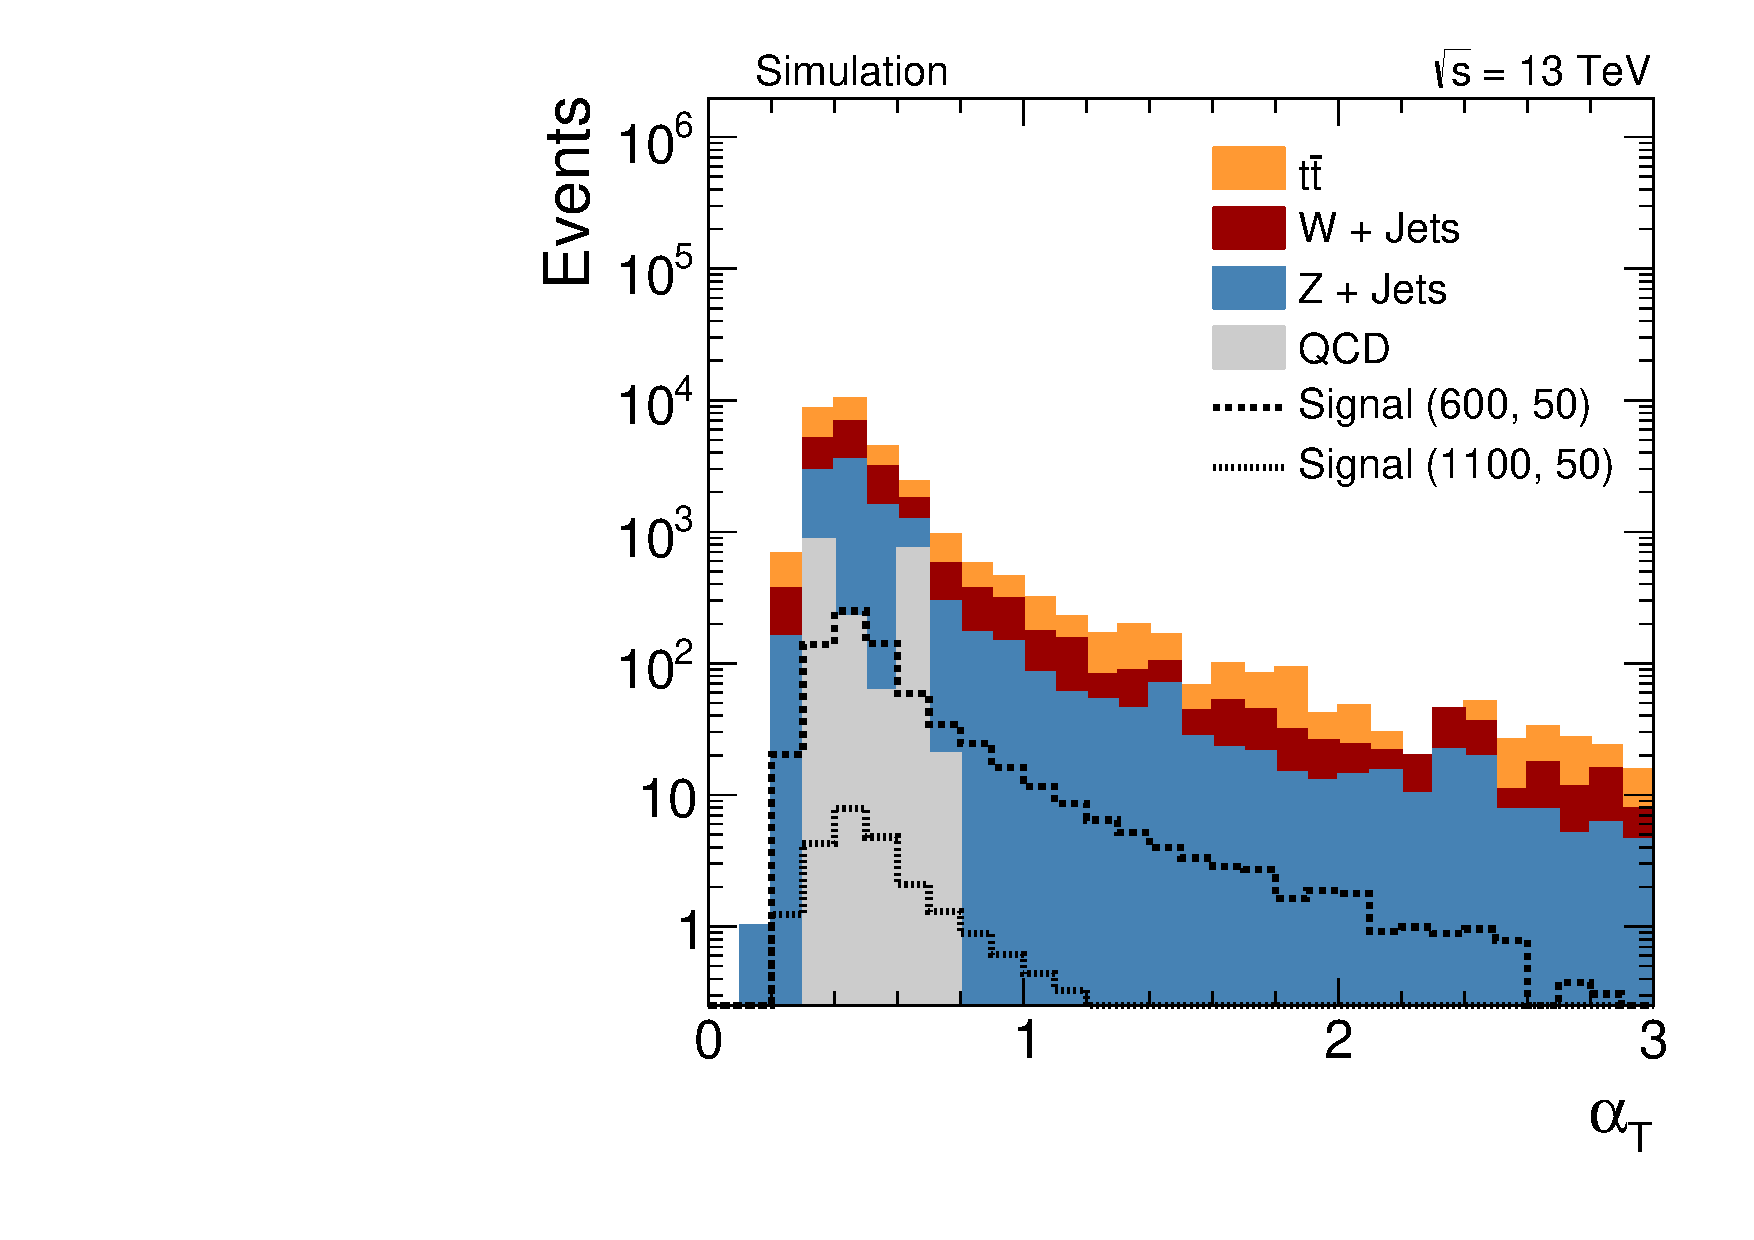
\includegraphics[width=0.49\textwidth]{figures/Stop_DeltaPhiSelection_AlphaT.pdf}  
      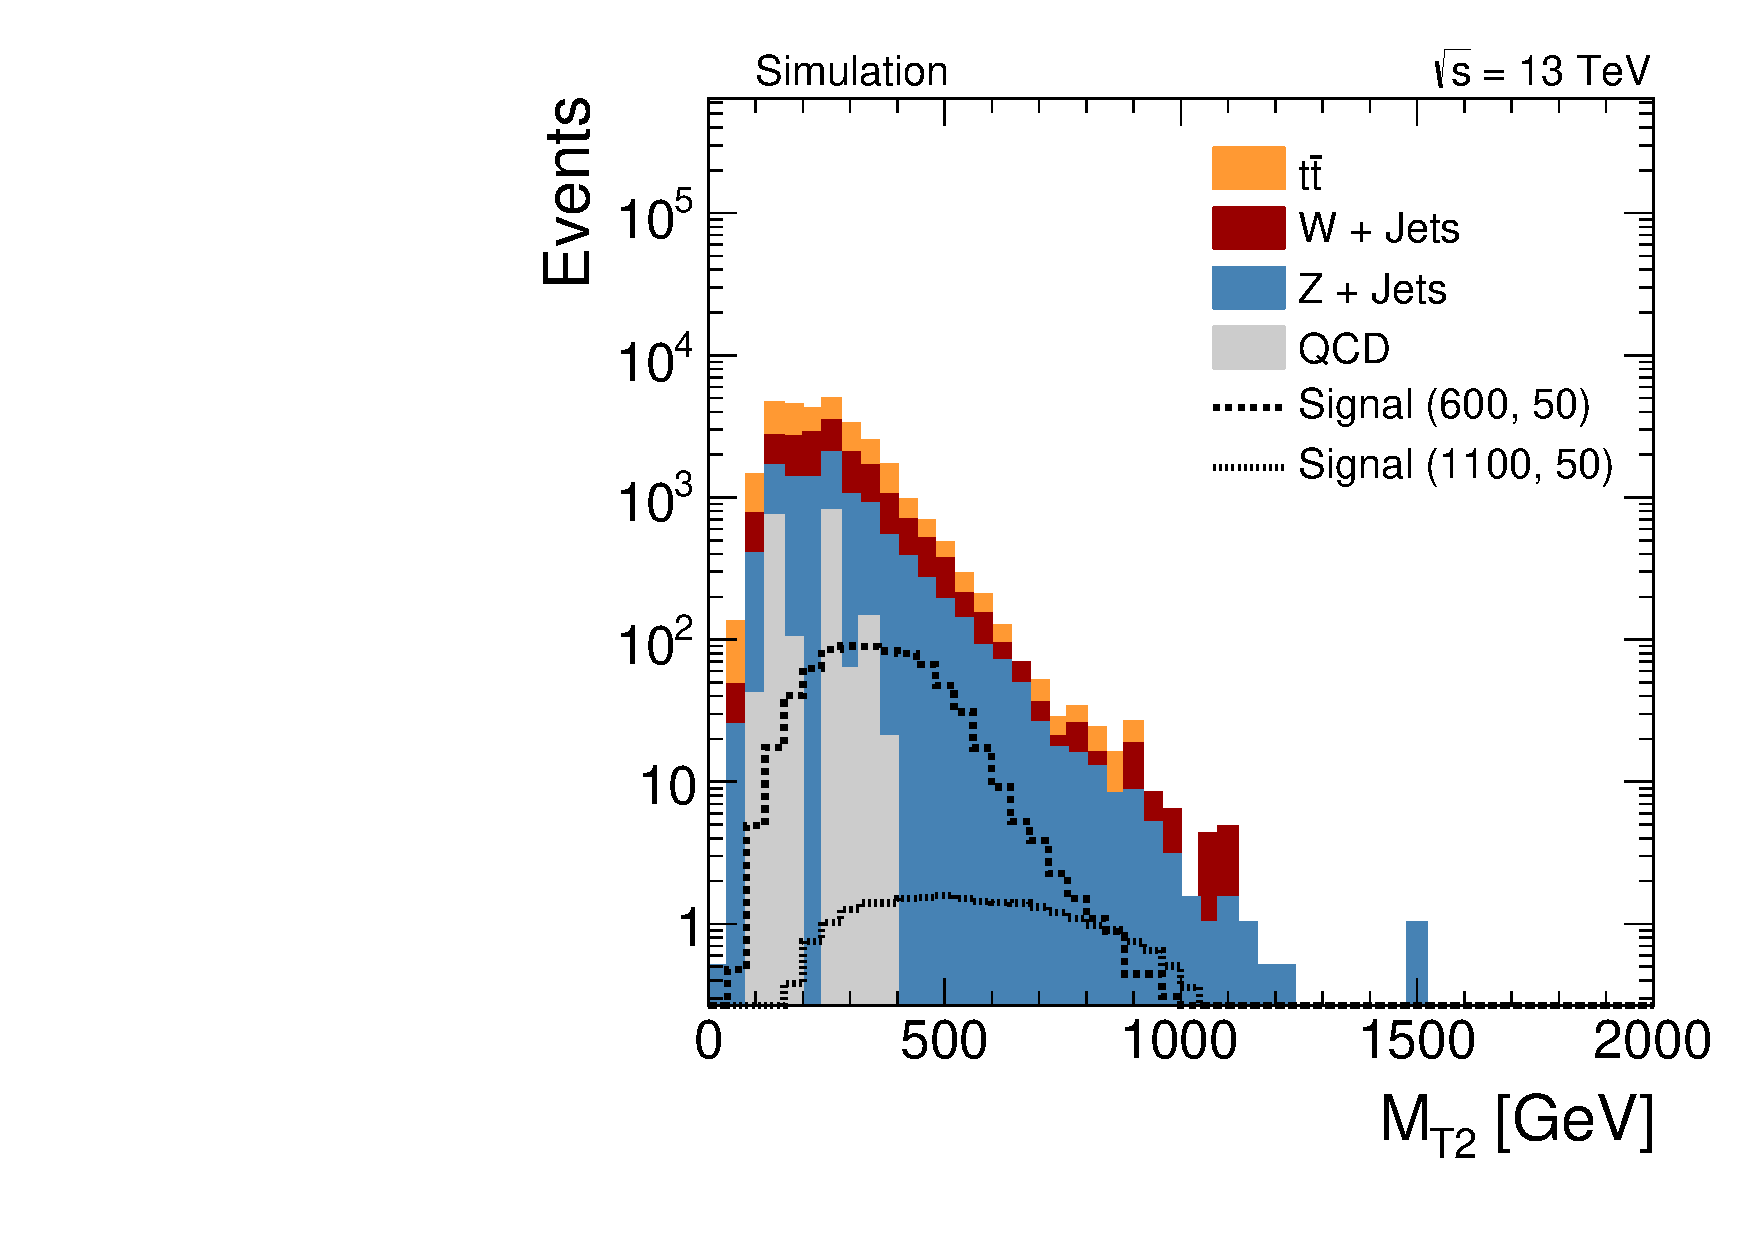
\includegraphics[width=0.49\textwidth]{figures/Stop_DeltaPhiSelection_MT2.pdf} \\
      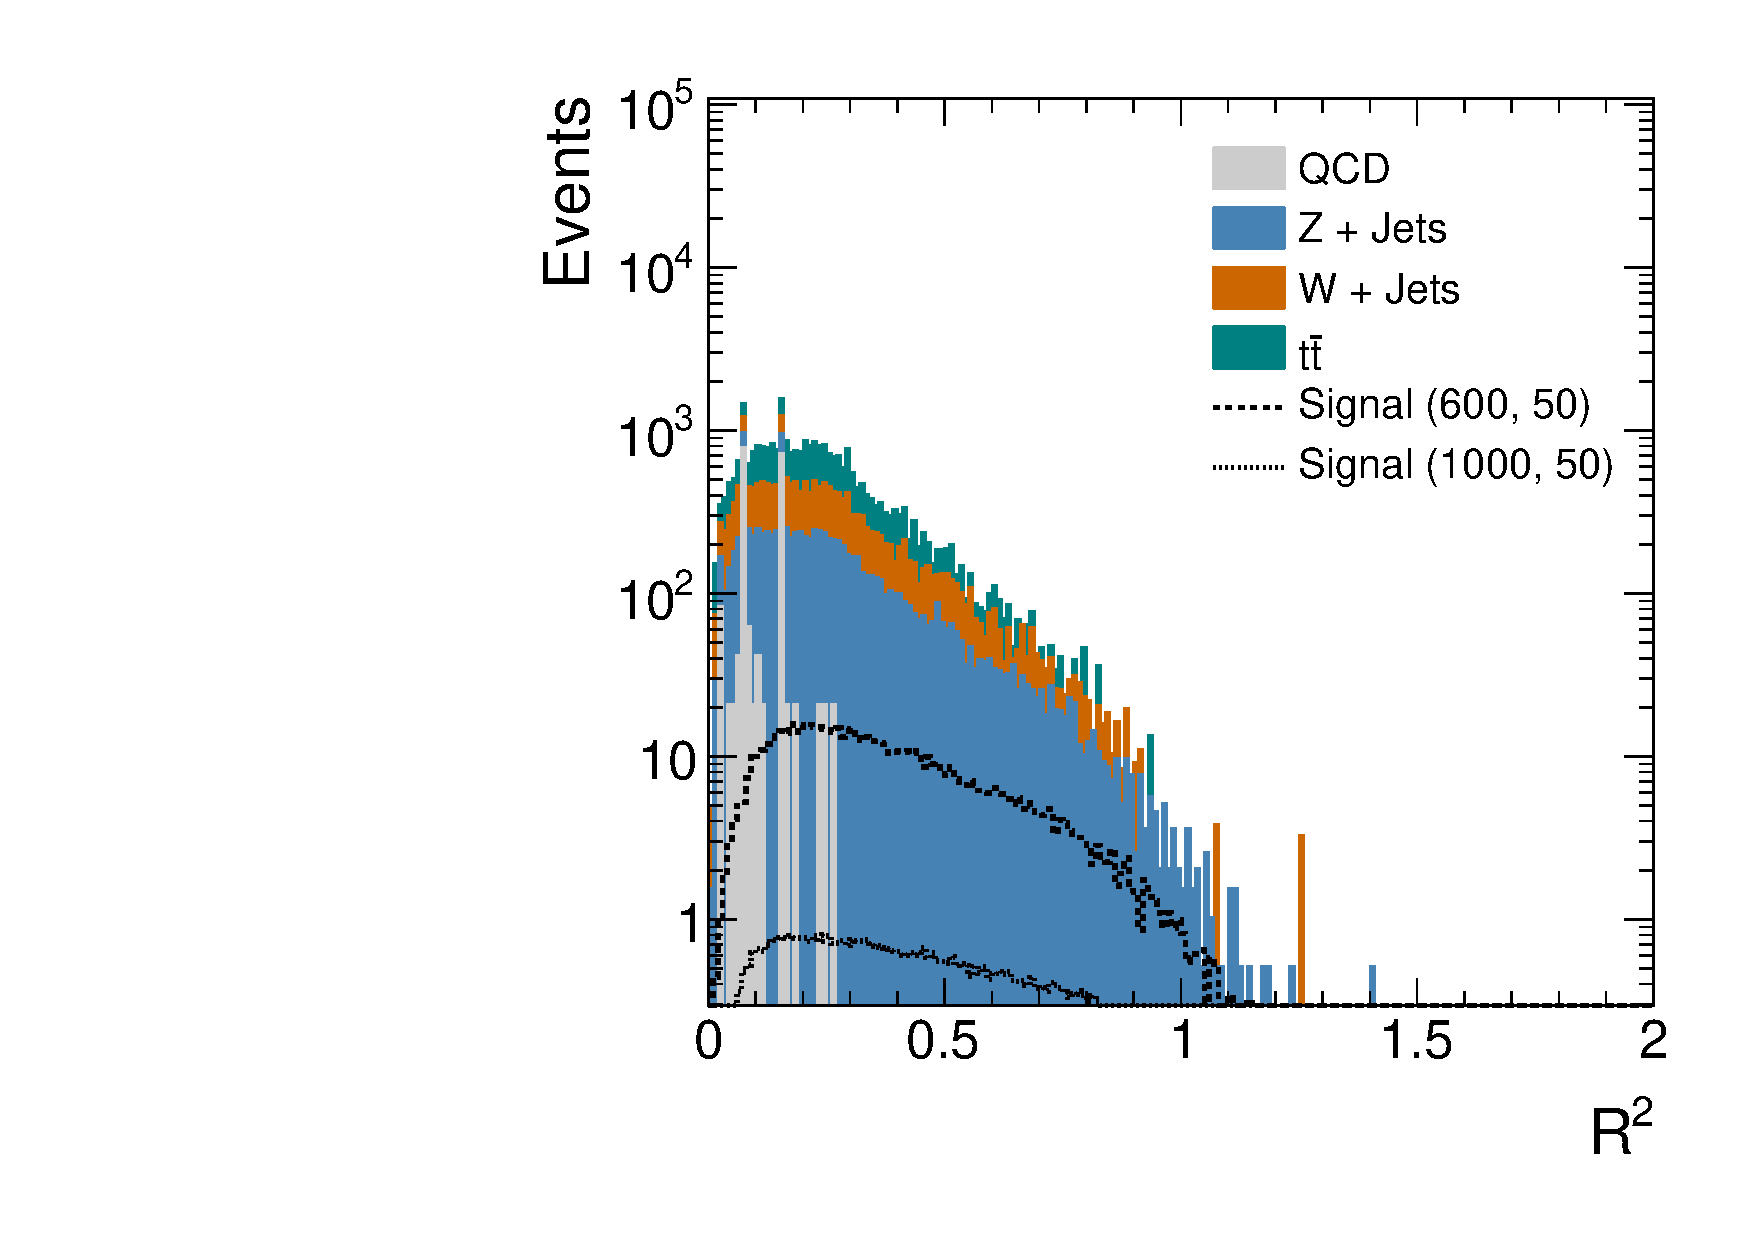
\includegraphics[width=0.49\textwidth]{figures/Stop_DeltaPhiSelection_Razor_R.pdf}
    \end{center}
  \end{minipage}

  \caption{Distribution of the $\alpha_T$ variable (\textit{top left}), $M_\mathrm{T2}$ (\textit{top right}) and  the razor variable $R^2$ (\textit{bottom}) after application of the baseline selection requirements for background and two selected signal samples. The signal points are labelled as (X, Y) where X is the stop quark mass and Y is the LSP mass in GeV.}
  \label{fig:stop_baseline_kin_vars}
\end{figure}
In addition to these variables, which are already well established in searches for supersymmetry, also other kinematic quantities can be considered:
\begin{description}
 \item \textbf{Transverse mass} $\mathbf{m_\mathrm{T}}$ \textbf{:} As shown in Fig.~\ref{fig:stop_top_channels}, background contributions from \ttbar events arise predominantly from semi-leptonic top quark decays. In such decays, the missing transverse energy mainly arises from the leptonically decaying top quark. This is caused by neutrinos from the decay of the $W$ boson and becomes even more prominent for lost-lepton events in which also the undetected lepton contributes to the missing energy. In both cases however, the missing energy is expected to point into the direction of the leptonic top decay accompanied by a b-quark jet also stemming from the top decay. Thus, the missing transverse energy and the closest b-tagged jet in $\Delta \phi$ can be utilized to calculate a transverse mass according to
\begin{equation}
m_\mathrm{T} = \sqrt{2 \pt^\mathrm{jet}\met \cdot (1-\mathrm{cos}(\Delta \phi(\mathrm{jet}, \met)))} \; .
\end{equation}   
The distribution obtained after applying the baseline selection is shown for background and two selected signal samples in Fig.~\ref{fig:stop_baseline_kin_vars2} (left). Here, the transverse mass is calculated from the missing transverse momentum and the closest b-tagged anti-$k_\mathrm{T}$ jet with $R = 0.5$ as identified by the CSV algorithm with medium working point and transverse momentum greater than 30\gev. The transverse mass is considered as zero in case no b-tagged jet could be identified. The distributions exhibit that this transverse mass variable has a peak in case of \ttbar events close to the top quark mass while it is shifted to higher values than the top-quark mass for signal events. 
 \item $\mathbf{\Delta \phi(CA}$--$\mathbf{jet_1, CA}$--$\mathbf{jet_2)}$ \textbf{:} The selection of events with a back-to-back topology has been used in Chap.~\ref{chap:Resolution} in order to identify dijet events by requiring $\Delta \phi > 2.7$. A similar situation can be expected to occur when having event topologies with boosted top quark decays in \ttbar events. For high transverse momenta, a \ttbar event features a dijet-like structure of two fat jets balanced against each other. For signal events however, such a topology is not expected, since the event is balanced against genuine \met arising from the LSPs. The selected $\Delta \phi$ distributions after applying baseline selection criteria are shown in Fig.~\ref{fig:stop_baseline_kin_vars2} (right).  
\end{description}
\begin{figure}[!t]
  \centering
  \begin{tabular}{cc}
                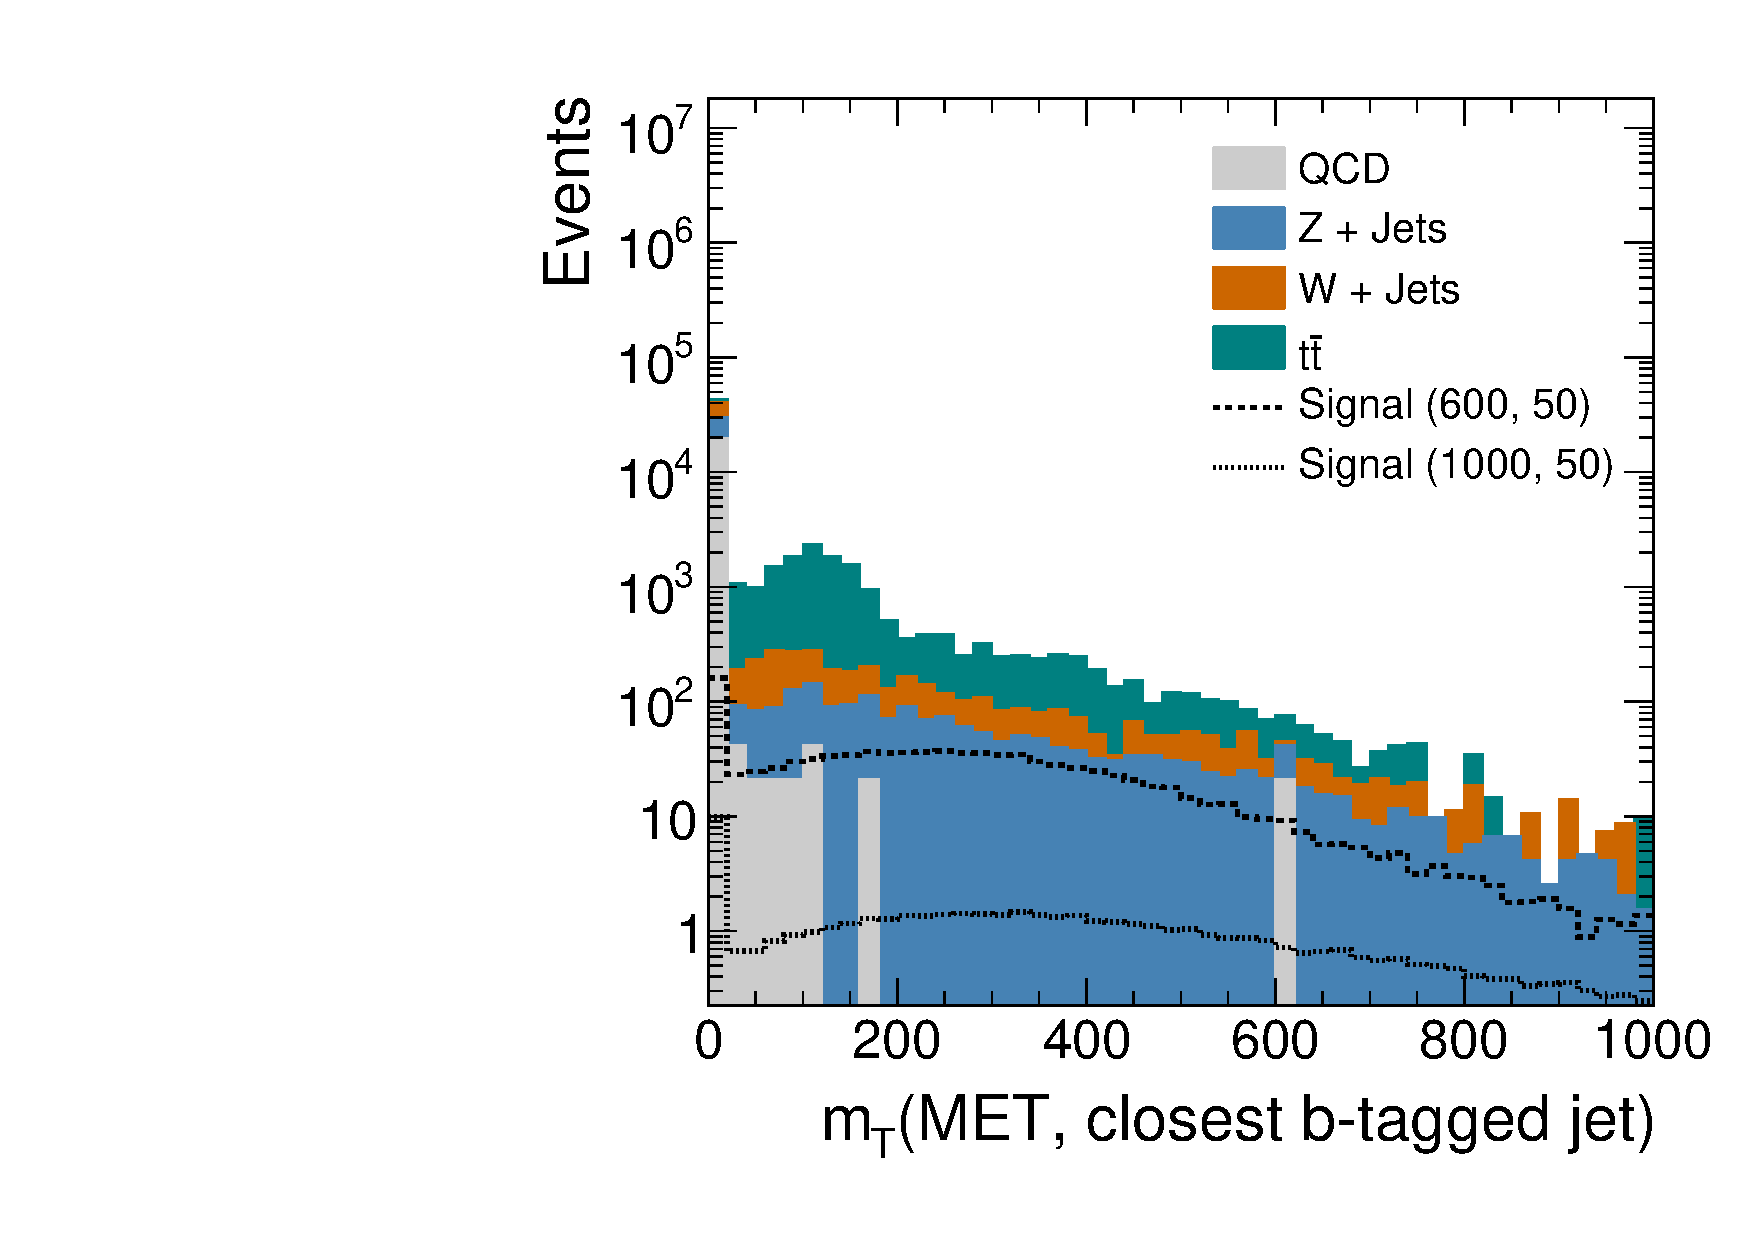
\includegraphics[width=0.49\textwidth]{figures/Stop_DeltaPhiSelection_transverseMass_MET_closestAndBTaggedJet.pdf} &
                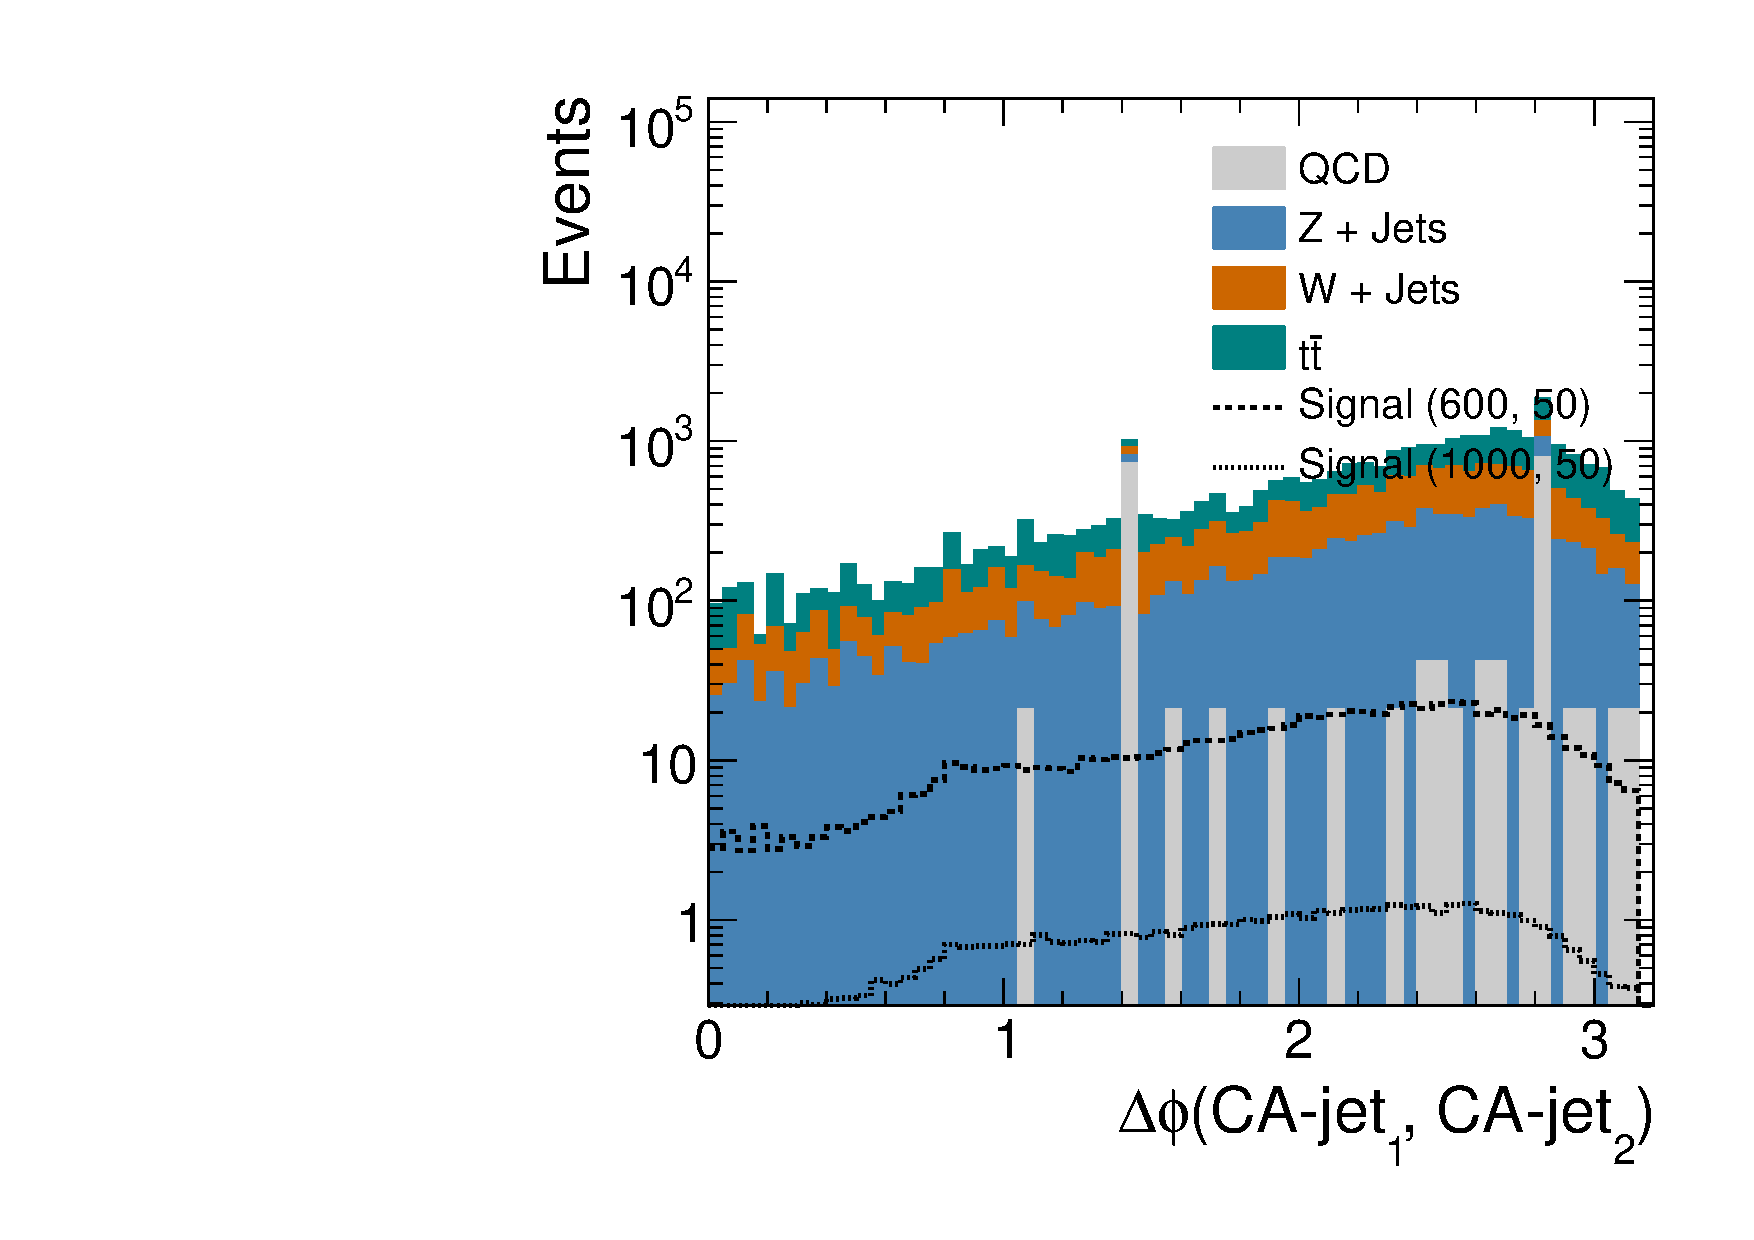
\includegraphics[width=0.49\textwidth]{figures/Stop_DeltaPhiSelection_deltaPhi_topjet1_topjet2.pdf}
  \end{tabular}
  \caption{Distribution of the $m_\mathrm{T}$ variable (\textit{left}) and $\Delta \phi(\mathrm{CA}$--$\mathrm{jet_1}, \mathrm{CA}$--$\mathrm{jet_2})$ (\textit{right}) after application of the baseline selection requirements for background and two selected signal samples. The signal points are labelled as (X, Y) where X is the stop quark mass and Y is the LSP mass.}
  \label{fig:stop_baseline_kin_vars2}
\end{figure}
In order to quantify the quality of these various kinematic selections, the separation power of the different variables is tested by studying again the background versus signal efficiency curves as introduced in Sec.~\ref{sec:stop_baseline}. The resulting curves after applying baseline selection criteria are shown in Fig.~\ref{fig:stop_baseline_cutscan_kin_vars}. For comparison, also the signal versus background efficiency curve for \met is illustrated. 
\begin{figure}[!t]
  \centering
\makebox[\linewidth]{
  \begin{tabular}{cc}
                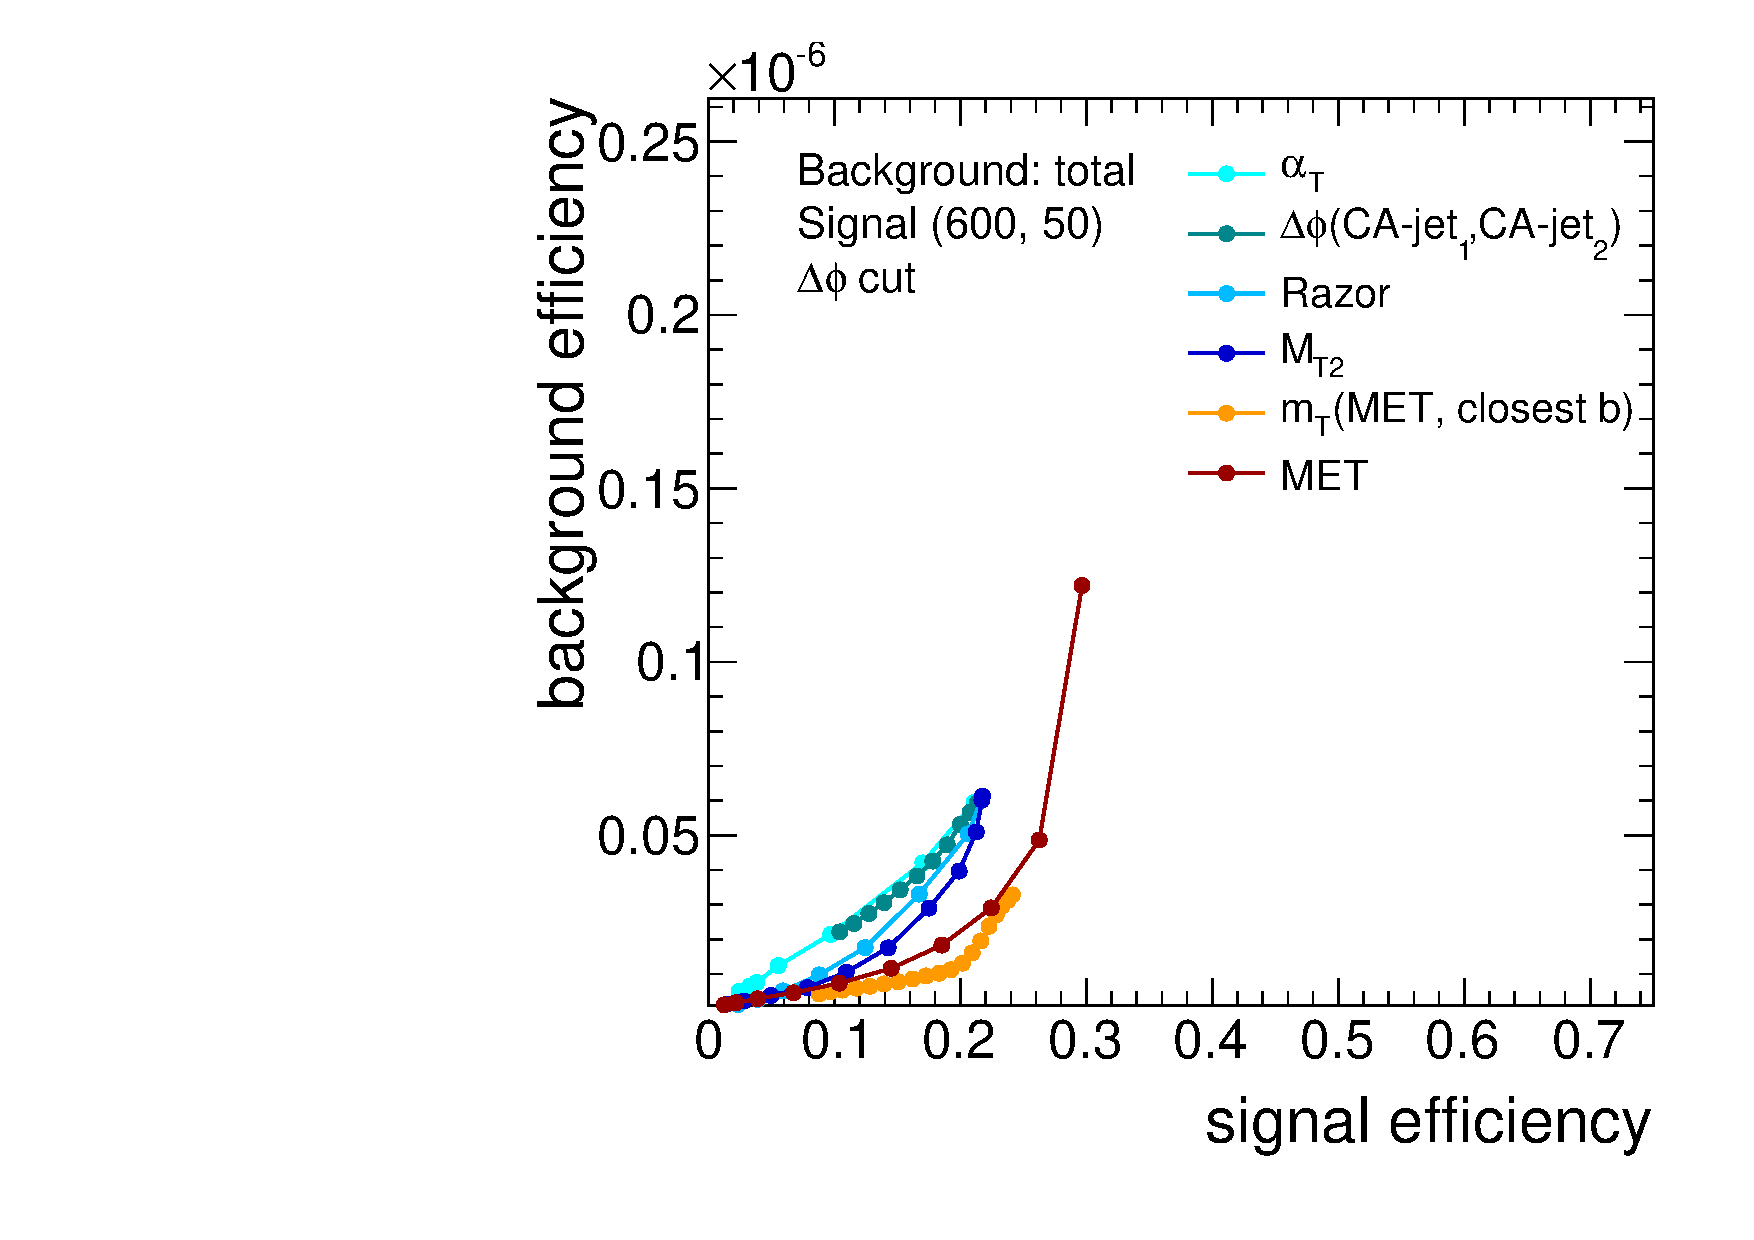
\includegraphics[width=0.49\textwidth]{figures/CutScan_DeltaPhiSelection_total_Stop600_LSP50_T2tt_13TeV_MT2_AlphaT_Razor_TopjetDeltaPhi_MET.pdf} & 
                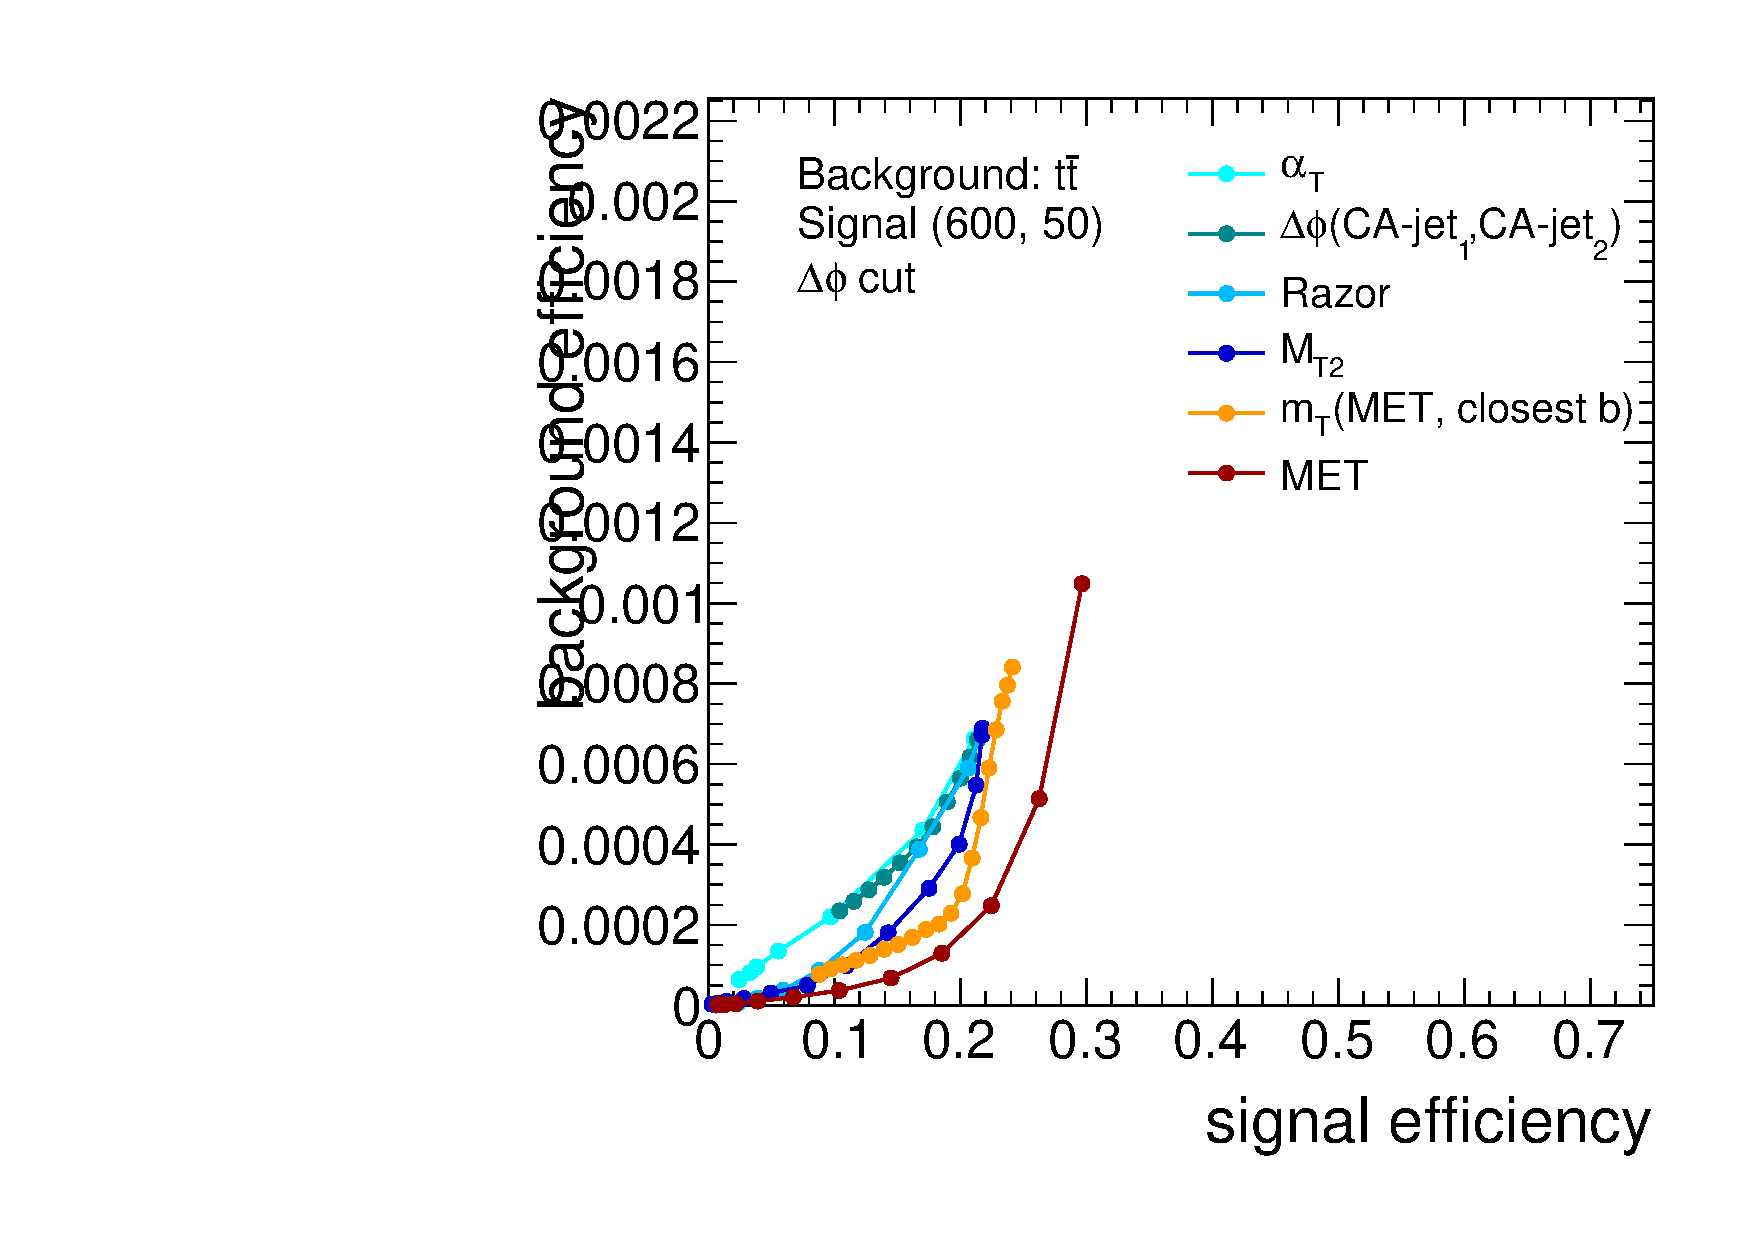
\includegraphics[width=0.49\textwidth]{figures/CutScan_DeltaPhiSelection_TTbar_powheg_13TeV_Stop600_LSP50_T2tt_13TeV_MT2_AlphaT_Razor_TopjetDeltaPhi_MET.pdf} \\
                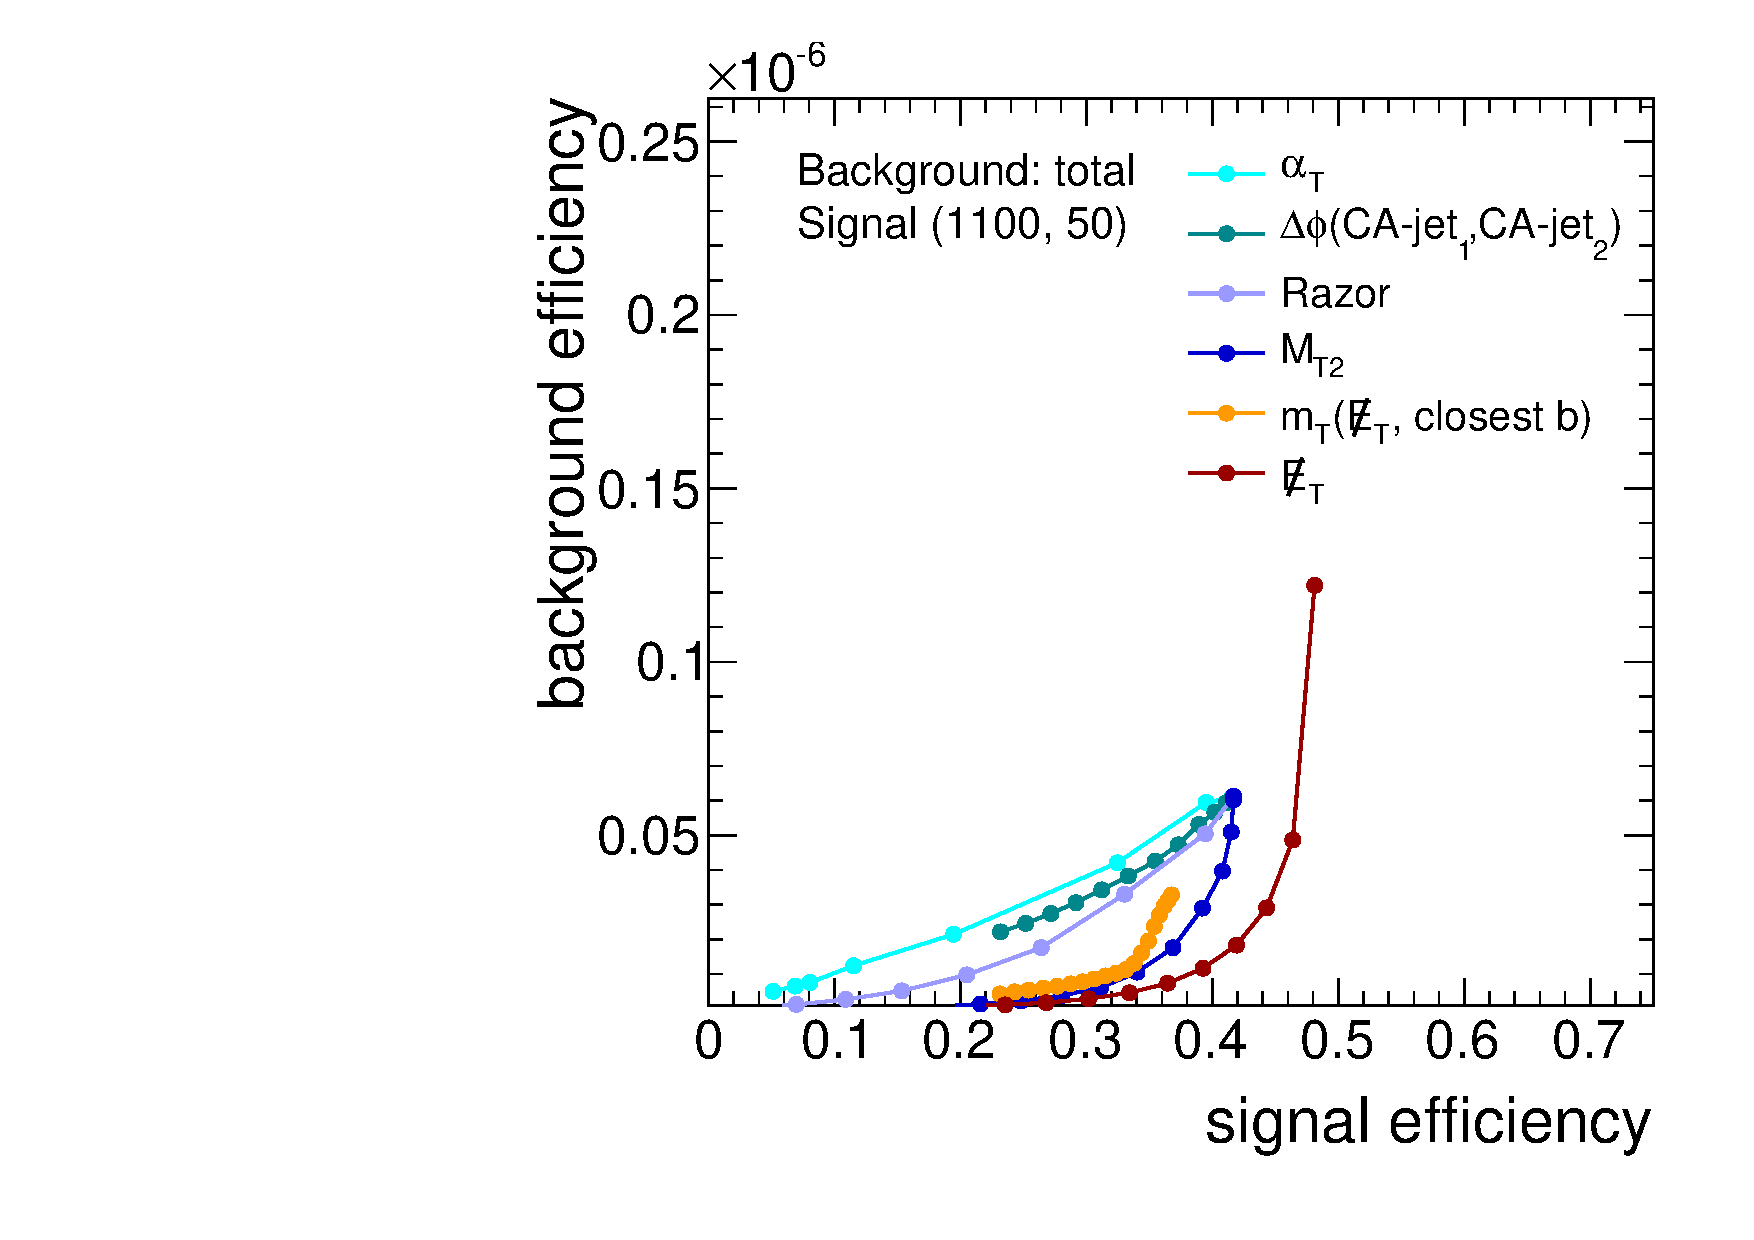
\includegraphics[width=0.49\textwidth]{figures/CutScan_DeltaPhiSelection_total_Stop1100_LSP50_T2tt_13TeV_MT2_AlphaT_Razor_TopjetDeltaPhi_MET.pdf} &
                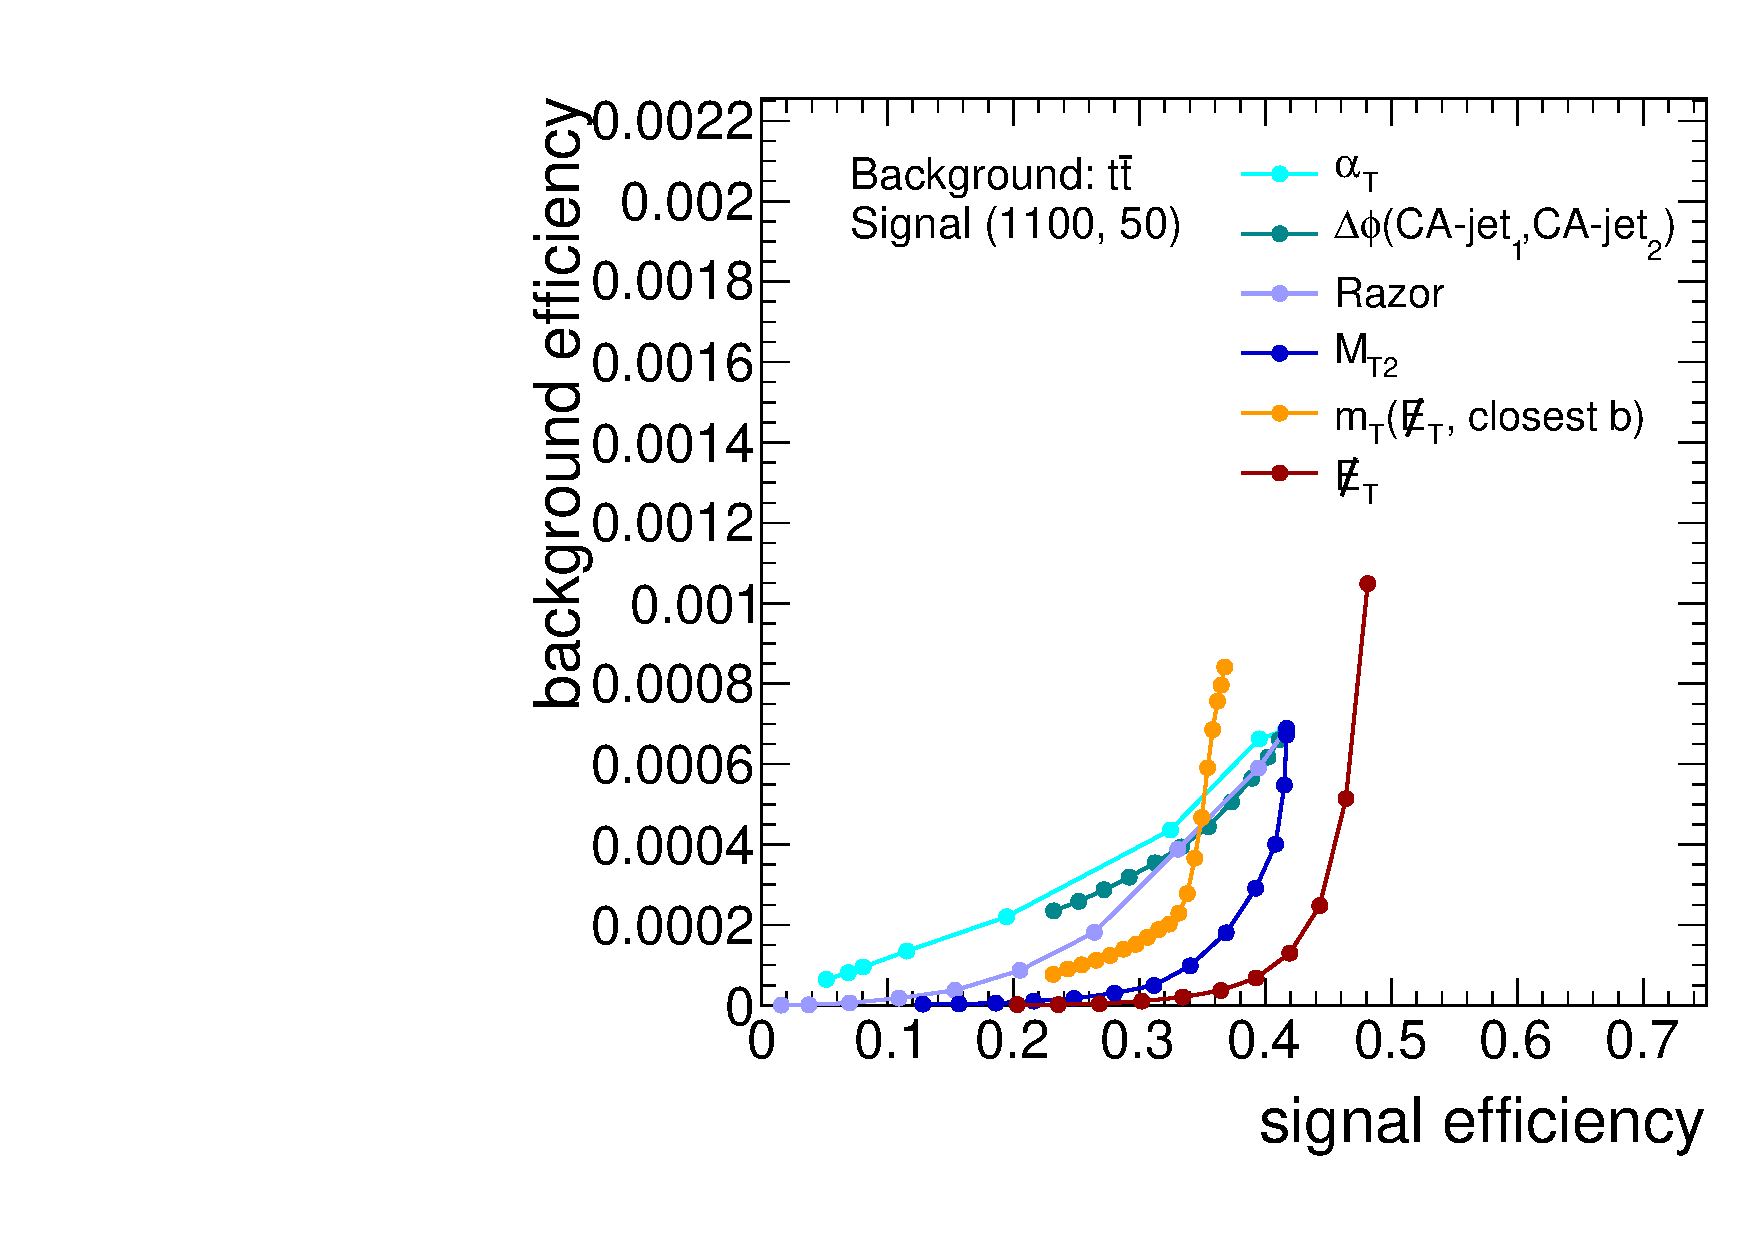
\includegraphics[width=0.49\textwidth]{figures/CutScan_DeltaPhiSelection_TTbar_powheg_13TeV_Stop1100_LSP50_T2tt_13TeV_MT2_AlphaT_Razor_TopjetDeltaPhi_MET.pdf}
  \end{tabular}}
  \caption{Evolution of the signal versus background efficiency for a stop mass of 600\gev (\textit{top}) and 1100\gev (\textit{bottom}) in case the background is the sum of all backgrounds (\textit{left}) or the \ttbar background (\textit{right}) after applying baseline selection criteria. The definitions of the variables $\alpha_\mathrm{T}$, $\Delta \phi(\mathrm{CA}$--$\mathrm{jet_1, CA}$--$\mathrm{jet_2})$, razor and $M_\mathrm{T2}$ imply a requirement of at least two CA-jets and the definition of $m_\mathrm{T}$ implies a requirement of at least one b-tagged jet.}
  \label{fig:stop_baseline_cutscan_kin_vars}
\end{figure}
\\
The calculation of $\alpha_\mathrm{T}$, $\Delta \phi(\mathrm{CA}$--$\mathrm{jet}_1, \mathrm{CA}$--$\mathrm{jet}_2)$, $M_\mathrm{T2}$ and the razor variable $R^2$ imply that there exist two CA8 jets with \pt$> 150$\gev in the event. Consequently, the starting point of that scan curves is different than that of the \met curve which represents the signal and background efficiencies after the baseline selection. Similarly the $m_\mathrm{T}$ curve implies that each event has at least one b-tagged jet. The point of highest efficiency for the $m_\mathrm{T}$ curve corresponds to a requirement of $m_\mathrm{T} > 20$\gev.  \\
The distributions exhibit that among the variables based on the presence of two CA8 jets, $M_\mathrm{T2}$ performs best, especially for high stop quark masses. This statement applies to the total background as well as to the \ttbar background only. Furthermore, the selection based on $m_\mathrm{T}$ shows a nice separation power as well and outperforms $M_\mathrm{T2}$ especially for smaller stop masses. It is visible that the curve for $m_\mathrm{T}$ shows a distinct kink. This corresponds to a selection keeping only events with $m_\mathrm{T}$ greater than the top quark mass. When imposing even tighter selection requirements on $m_\mathrm{T}$, the separation power decreases rapidly. \\
In order to compare the quality of these different criteria not only for the total signal and background efficiencies, the signal over background ratios are summarized in Tab.~\ref{tab:stop_kin_sel_soverb} for the four different search regions. 
\begin{table}[!t]
\fontsize{9 pt}{1.2 em}
\selectfont
\centering
\caption{Signal over background ratios are displayed for two signal points labelled as (X, Y), where X is the stop quark mass and Y is the LSP mass in GeV, in the four exclusive search regions. For definitions of selections see text. }
\makebox[\linewidth]{
\begin{tabular}{llrrrr}
\multicolumn{6}{c}{} \\
  \toprule 
   &  & \multicolumn{4}{c}{S/B}\\
   \midrule
   &  & top tag & top tag + $M_\mathrm{T2}$ & top tag + b tag & top tag + $m_\mathrm{T}$ \\
   \midrule
 \multirow{2}{*}{SR1} & Signal (600, 50) & 0.04 & 0.2 & 0.05 & 0.1 \\
                      & Signal (1100, 50) & 0.0004 & 0.002 & 0.0004 & 0.001 \\
                      \midrule
 \multirow{2}{*}{SR2} & Signal (600, 50) & 0.3 & 0.3 & 0.5 & 0.7 \\
                      & Signal (1100, 50) & 0.008 & 0.01 & 0.01 & 0.02 \\
                      \midrule
 \multirow{2}{*}{SR3} & Signal (600, 50) & 0.08 & 0.2 & 0.1 & 0.2 \\ 
                      & Signal (1100, 50) & 0.003 & 0.01 & 0.003 & 0.007 \\
                      \midrule
 \multirow{2}{*}{SR4} & Signal (600, 50) & 0.6 & 0.8 & 1.1 & 2.7 \\  
                      & Signal (1100, 50) & 0.1 & 0.2 & 0.2 & 0.5 \\
  \bottomrule
\end{tabular}}
\label{tab:stop_kin_sel_soverb}
\end{table}   
Here, the signal over background ratios are shown for the baseline selection including at least one CMS top-tagged jet (denoted \textit{top tag}) and when adding in addition to these requirement $M_\mathrm{T2} > 400$\gev (\textit{top tag + $M_\mathrm{T2}$}), at least one b-tagged jet (\textit{top tag + b tag}) or $m_\mathrm{T} > 180$\gev (\textit{top tag + $m_\mathrm{T}$}). Although the signal versus background efficiency curves have indicated that the selection including $M_\mathrm{T2}$ provides the best signal to background ratios when considering the whole sample, the signal to background ratios for distinct search regions are highest in case a selection with $m_\mathrm{T}$ is used. For a further quantification, expected exclusion curves are derived again based on the same exclusive search regions, as defined in Tab.~\ref{tab:stop_excl_search_bins}, considering the uncertainties for each background source, as described in Sec.~\ref{sec:stop_baseline}. In Fig.~\ref{fig:stop_baselinetoptag_limit}, the derived expected exclusion limits are compared for various selections as a function of the stop quark mass for a LSP mass of 50\gev. The selection discussed in Sec.~\ref{sec:stop_btagging}, in which at least one CMS top tag is required in addition to the baseline selection, is illustrated in light green. This selection is combined with either a selection of $M_\mathrm{T2} > 400$\gev (pink), a b-tag requirement as discussed already in Sec.~\ref{sec:stop_btagging} (dark green) or a requirement of $m_\mathrm{T} > 180$\gev (light blue). It turns out that the latter performs best among those described selections over the whole stop mass range, as indicated already by the achieved signal to background ratios. 
\begin{figure}[!h]
  \centering
  \begin{tabular}{c}
                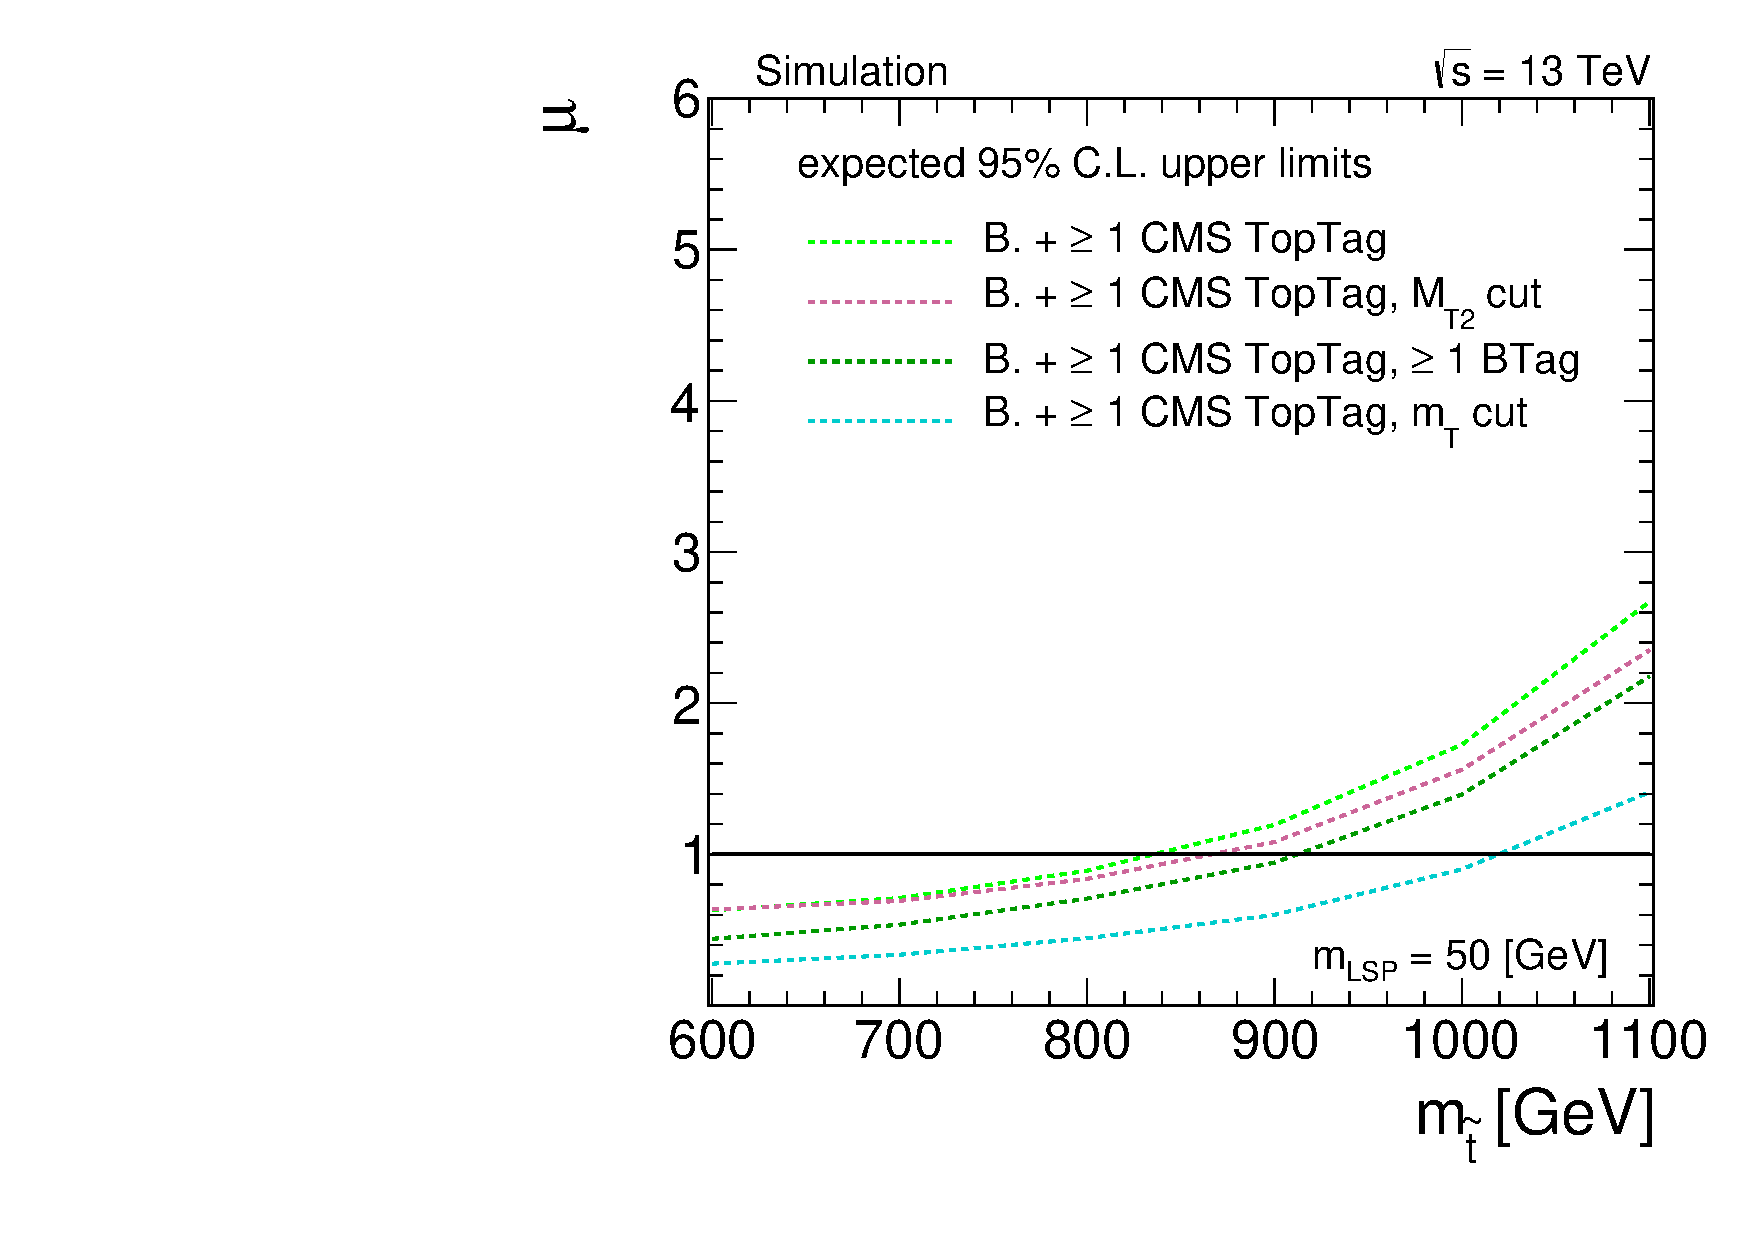
\includegraphics[width=0.49\textwidth]{figures/limitplot4BinSel_BaselineBTagTopTagTransverseMassMT2_LSP50.pdf} 
  \end{tabular}
  \caption{Expected 95\% upper limit for signal strength versus $m_{\tilde{t}}$. The LSP mass is chosen to be 50\gev. The label B. denotes the baseline selection.}
  \label{fig:stop_baselinetoptag_limit}
\end{figure}

\section[Performance Comparison to Selection Based on Published Stop Analysis]{Performance Comparison to Selection Based on Published Stop Analysis at $\mathbf{\sqrt{s} = 8}$\tev}
\label{sec:stop_pub}
In order to get a better understanding of the quality of the studied selections, a comparison to the analysis criteria used in SUS-13-015 is carried out in this section. \\
The comparison is done by performing the same selections as done in SUS-13-015 based on the simulated samples discussed in Sec.~\ref{sec:stop_samples}. Jets in this analysis are clustered with the anti-$k_T$ algorithm with a distance parameter of $R = 0.5$ and corrected for pileup effects by applying charged-hadron subtraction. The pre-selection criteria used here are:
\begin{itemize}
 \item Events with isolated electrons and muons with \pt$ > 10$\gev, as described in Sec.~\ref{sec:stop_baseline}, are vetoed.
 \item Events have to have at least five jets with \pt$ > 30$\gev and $|\eta| < 2.4$. The two highest \pt jets further have to have \pt$> 70$\gev while the next two highest jets in \pt must fulfill \pt$ > 50$\gev.
 \item There has to be at least one b-tagged jet in the event based on the CSV algorithm with medium working point. 
 \item The minimum azimuthal angle between the three highest jets and the missing transverse momentum has to be $\Delta \phi(\mathrm{jet}_n, \met) > 0.5$, $n = 1,2$ and $\Delta \phi(\mathrm{jet}_3, \met) > 0.3$.\footnote{The missing transverse energy in the published analysis is denoted with $\pt^\mathrm{miss}$.}% However, just like \met, it is the magnitude of the negative vector sum of the transverse momenta of all particles reconstructed in the event.}
\end{itemize}
The only difference between these selection criteria employed here and SUS-13-015 is related to the lepton veto. While in SUS-13-015 it is required to have no events with identified and isolated electrons and muons with \pt$> 5$\gev, here only events with electrons and muons with \pt$> 10$\gev are vetoed. However, since the 10\gev lepton veto is the same lepton veto requirement as for the other selections studied in this chapter, it is easier to compare the quality of the different selections applied to the sample after selecting the all-jet final state. In addition to those pre-selection requirements, further selection criteria are imposed in order to reconstruct the hadronically-decaying top quarks. The set of five or more jets in the event is separated into all possible combinations of three jets and a remnant containing at least one b-tagged jet. These sets are used to reconstruct the two expected top quarks in the event: one is based on one of the trijet combinations and denoted \textit{fully-reconstructed} top (denoted \textit{3-jet}) while the other is based on the remnant system and referred to as \textit{partially-reconstructed} top (denoted \textit{Rsys}). Details on the reconstruction process of the two top quark systems can be found in~\cite{CMS-PAS-SUS-13-015}. In particular, this process involves that the fully-reconstructed top quark has to satisfy the criteria described in Eq.~\ref{eq:hep_1},~\ref{eq:hep_2} and~\ref{eq:hep_3} using $R_\mathrm{min} = 0.85 \cdot (m_W/m_\mathrm{top})$, $R_\mathrm{max} = 1.25 \cdot (m_W/m_\mathrm{top})$, $m_W = 80.4$\gev and $m_\mathrm{top} = 173.1$\gev. If there is more than one trijet system satisfying these criteria the combination with $m^{3-\mathrm{jet}}$ closest to $m_\mathrm{top}$ is selected. 
\begin{figure}[!t]
  \centering
\makebox[\linewidth]{
  \begin{tabular}{cc}
                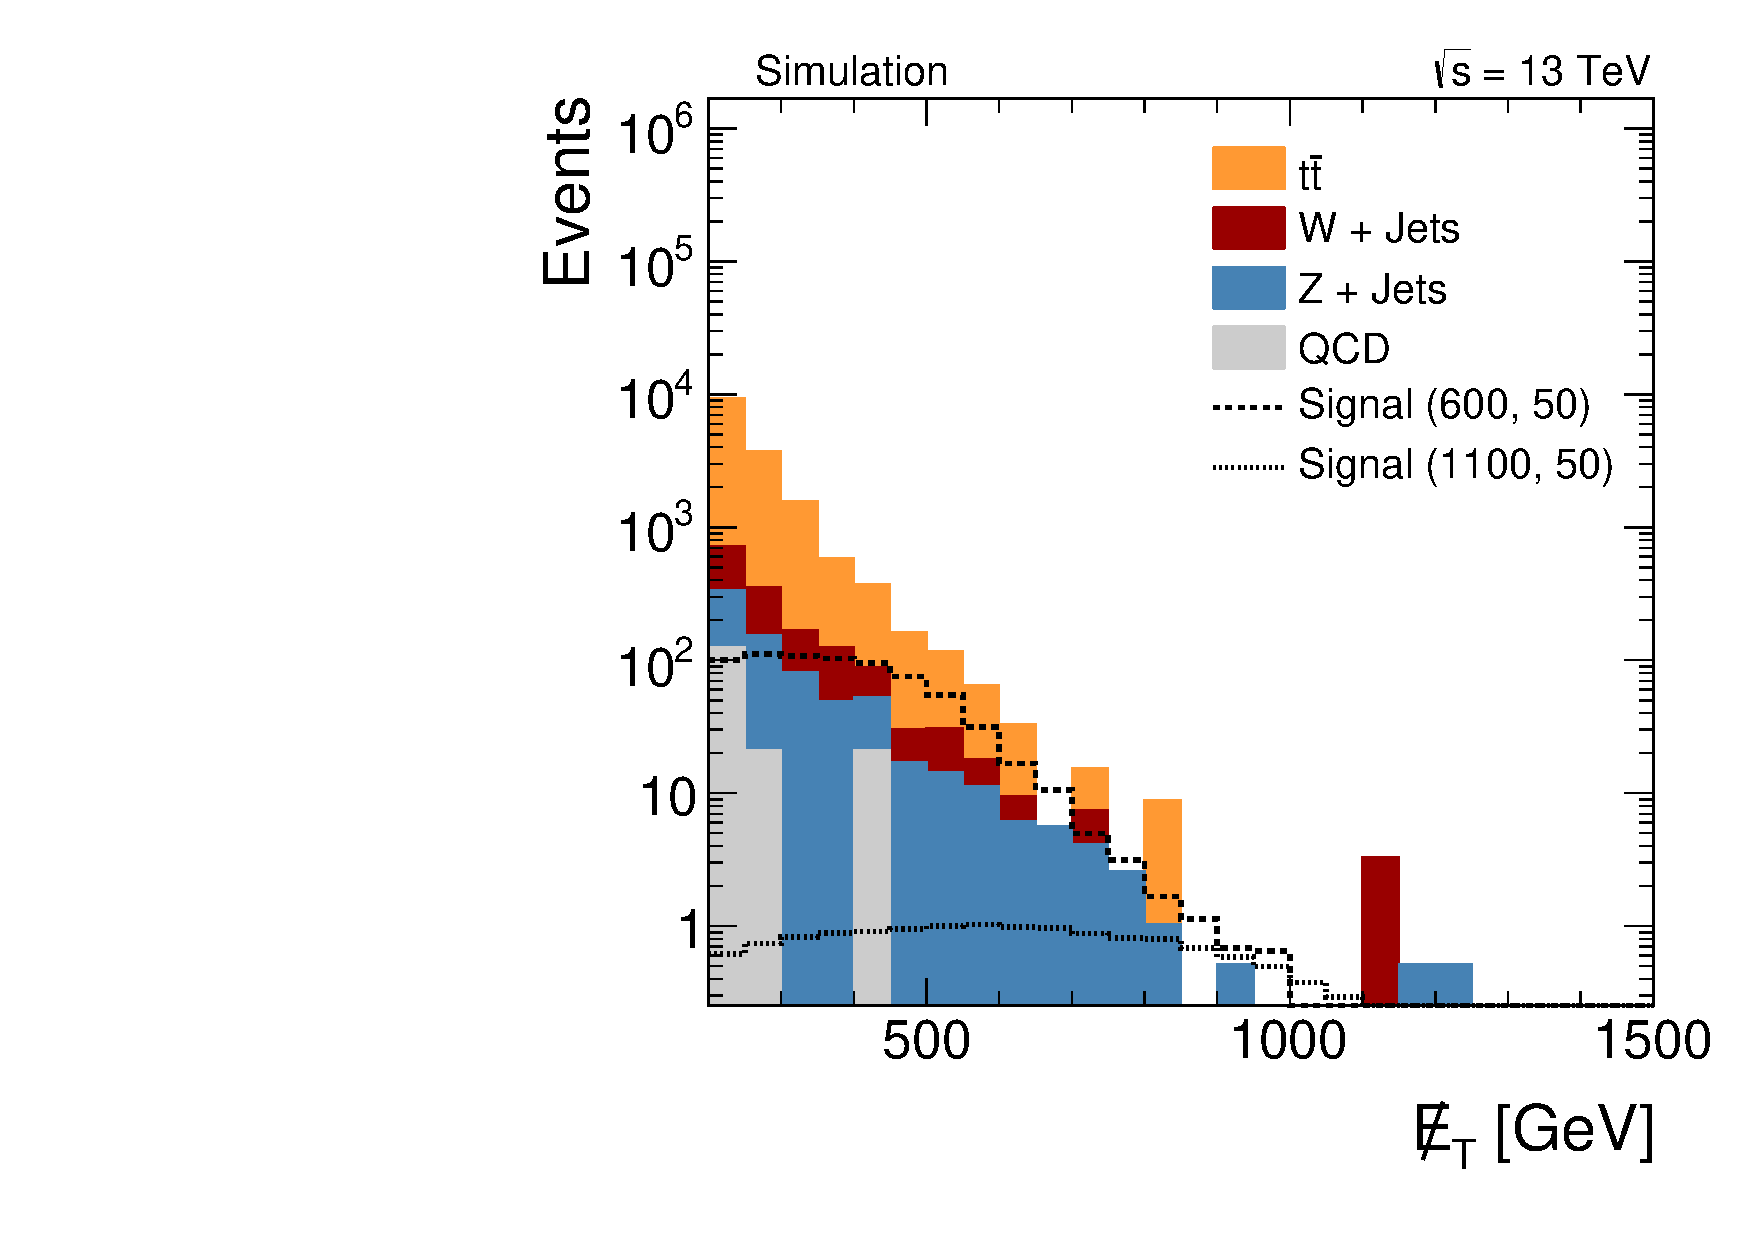
\includegraphics[width=0.49\textwidth]{figures/ReferenceStop_METSelection_MET.pdf} & 
                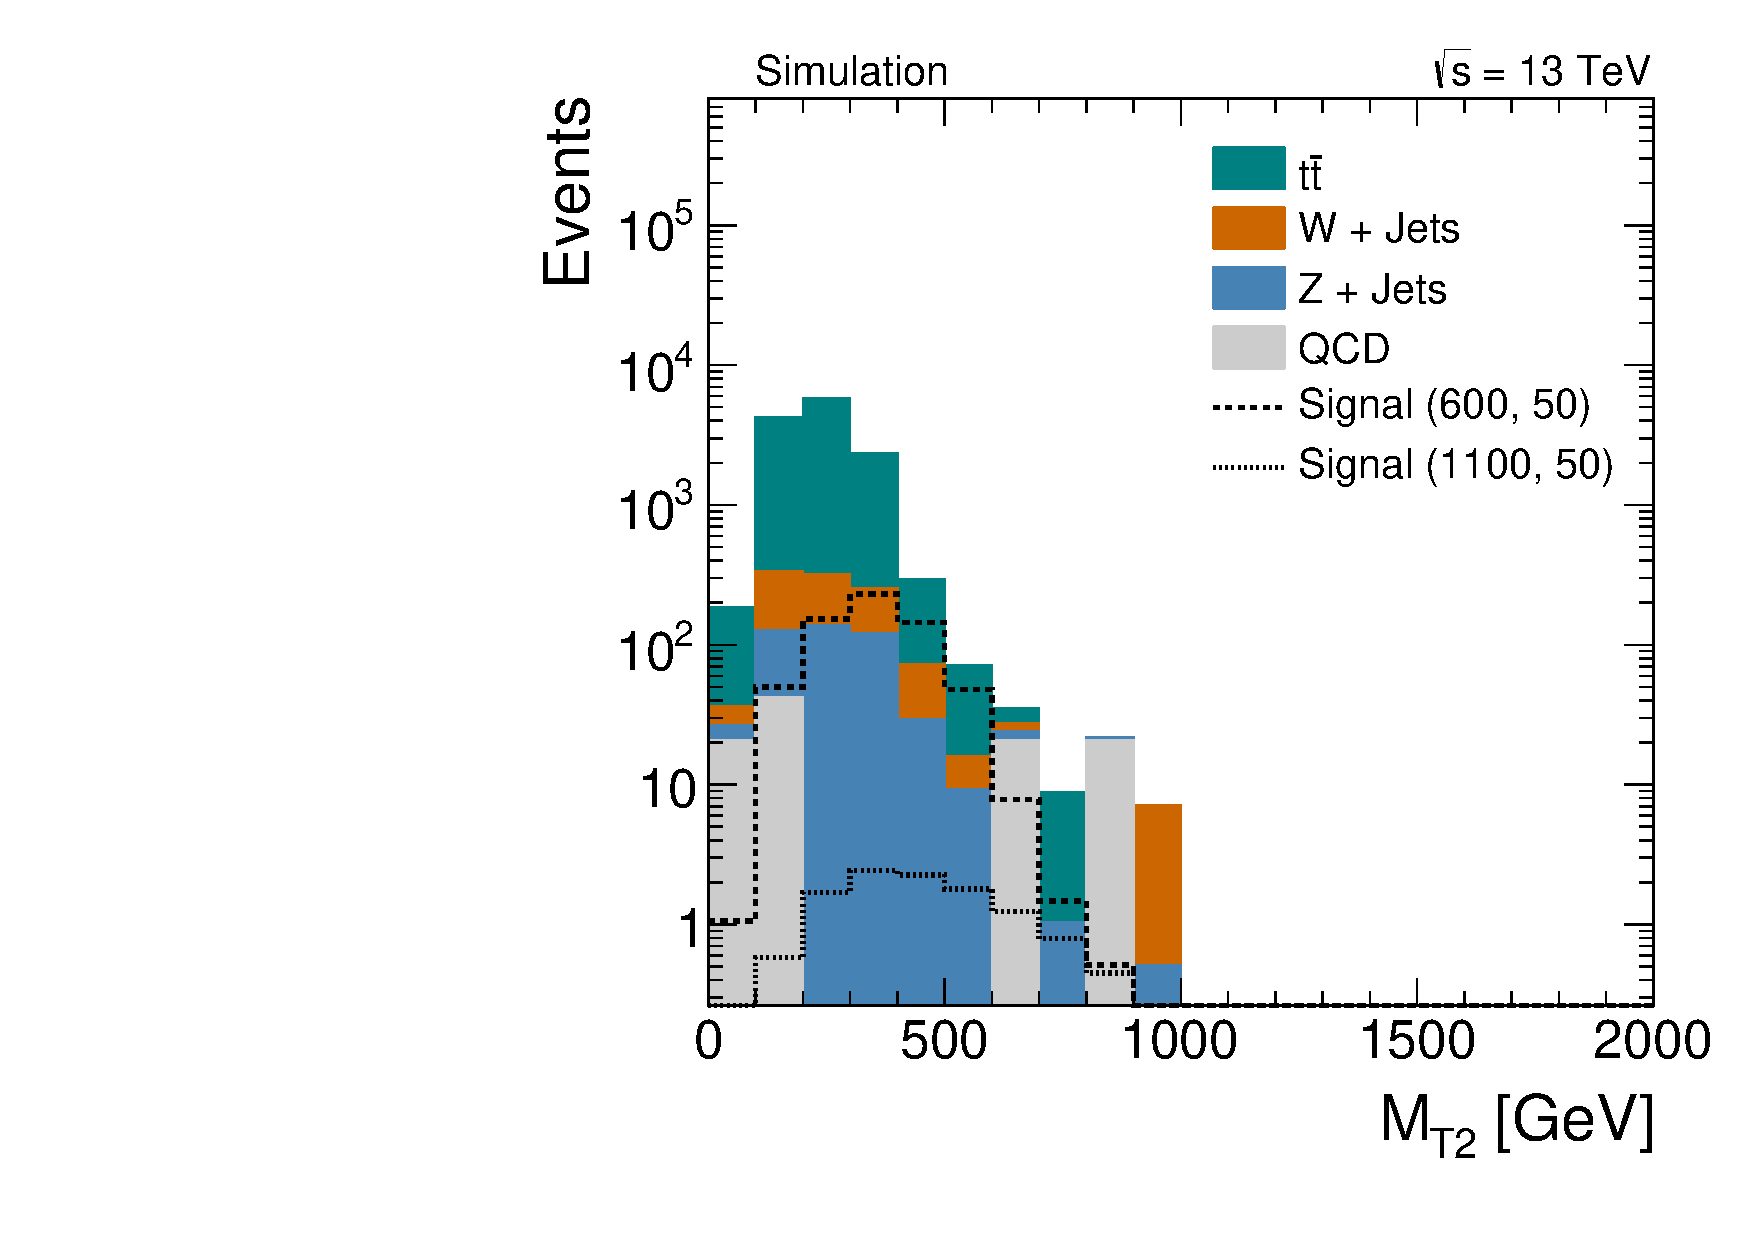
\includegraphics[width=0.49\textwidth]{figures/ReferenceStop_METSelection_ref_MT2.pdf} \\
                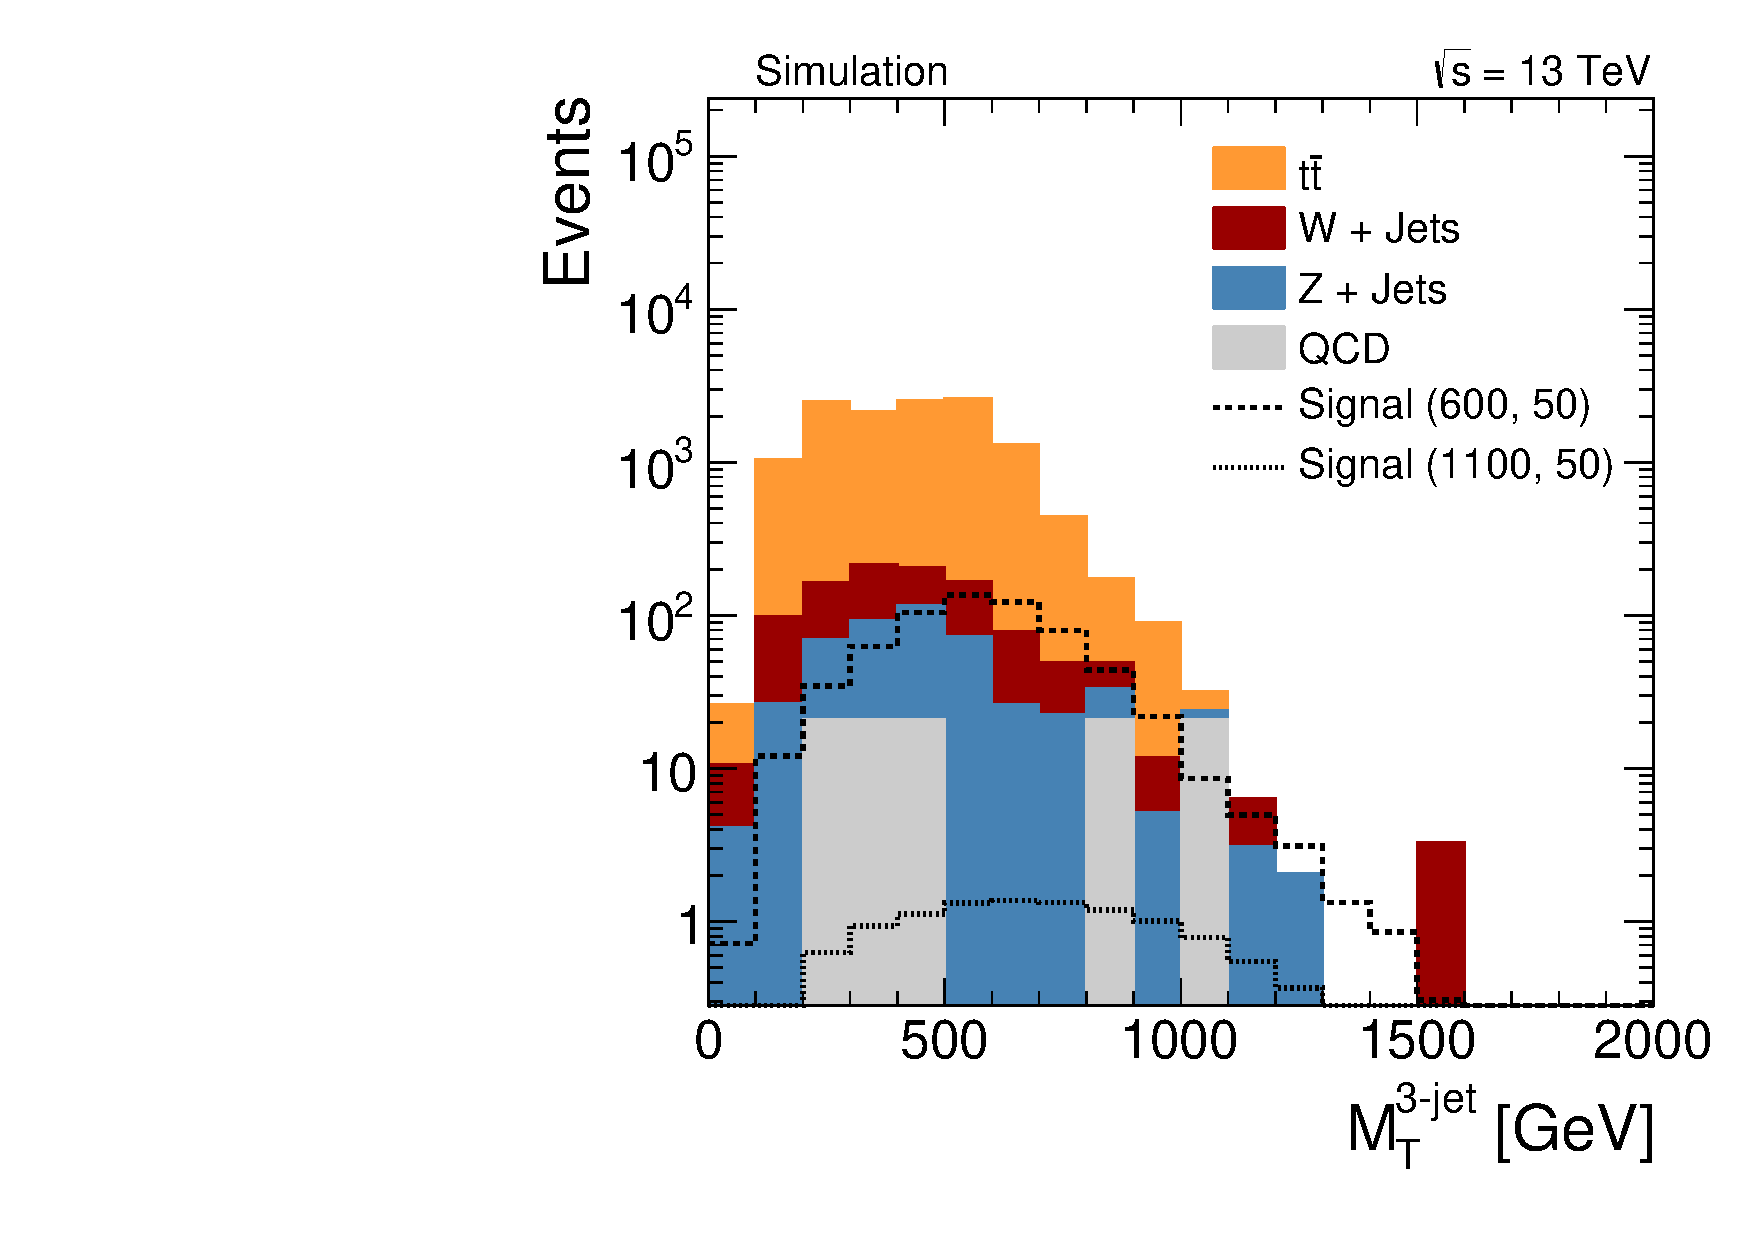
\includegraphics[width=0.49\textwidth]{figures/ReferenceStop_METSelection_ref_Mt3jet.pdf} & 
                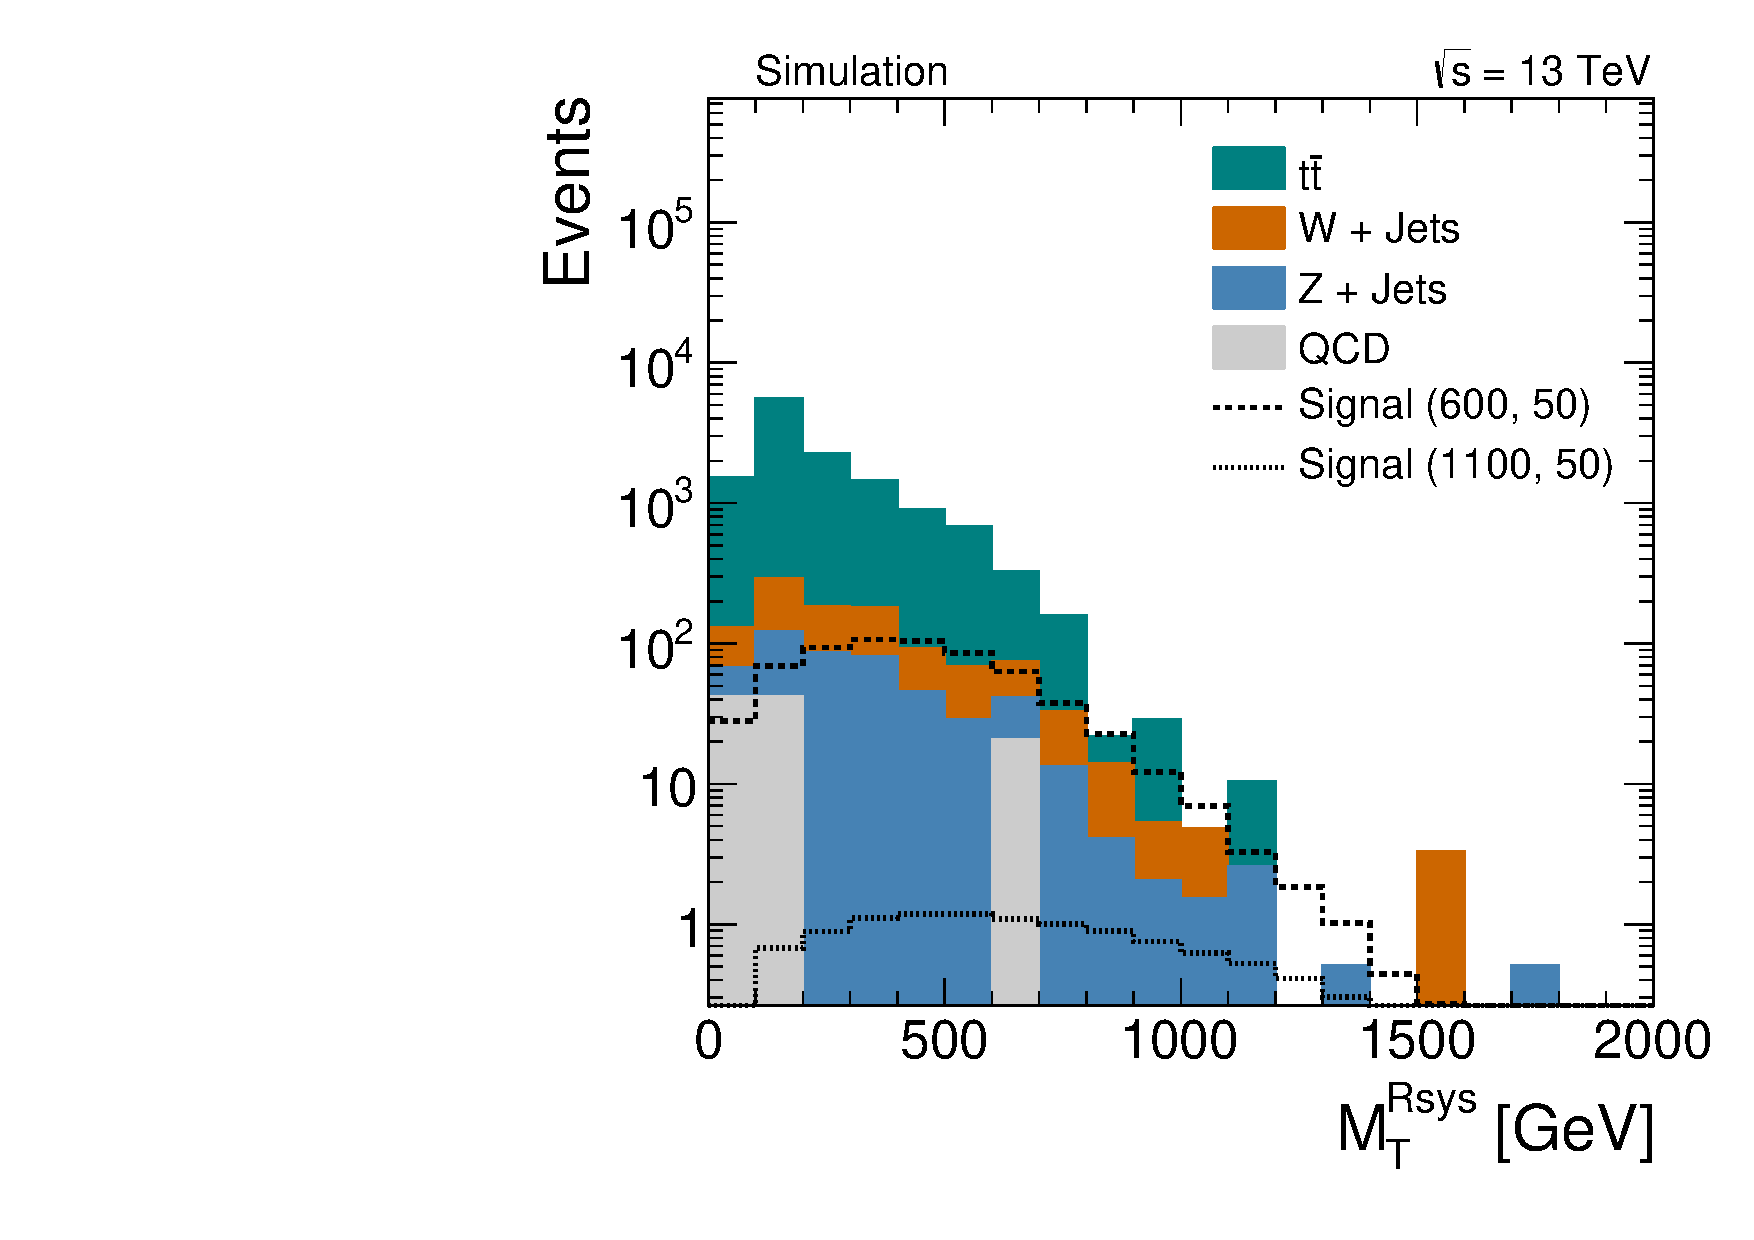
\includegraphics[width=0.49\textwidth]{figures/ReferenceStop_METSelection_ref_MtRsys.pdf}
  \end{tabular}}
  \caption{Comparison of \met, $M_\mathrm{T2}$, $M_\mathrm{T}^\mathrm{3-jet}$ and $M_\mathrm{T}^\mathrm{Rsys}$ distributions for signal and background events after applying pre-selection criteria and $\met > 200$\gev. The signal points are labelled as (X, Y) where X is the stop quark mass and Y is the LSP mass in GeV.}
  \label{fig:stop_ref_plots}
\end{figure} 
\\
After the successful identification of the two top quark systems according to the above mentioned criteria, further topological requirements are used:
\begin{itemize}
 \item \met $> 200$\gev
 \item The variable $M_\mathrm{T2}$, as discussed in Sec.~\ref{sec:stop_cuts}, is required to be $\ge 300$\gev. It is calculated from the four momenta of the fully- and the partially-reconstructed top quark as well as \met assuming the invisible particles to be massless. 
 \item $(0.5 \cdot M_\mathrm{T}^\mathrm{3-jet} + M_\mathrm{T}^\mathrm{Rsys}) \ge 500$\gev. $ M_\mathrm{T}^\mathrm{3-jet}$ and $M_\mathrm{T}^\mathrm{Rsys}$ denote the transverse mass of the fully-reconstructed and the remnant system which are calculated with the angle $\Delta \phi$ between the missing energy and the momentum vector of the three-jet or remnant system, respectively, according to
\begin{equation*}
( M_\mathrm{T}^\mathrm{3-jet})^2 = (m^{3-\mathrm{jet}})^2 + 2(E_\mathrm{T}^\mathrm{3-jet} \, \met - p_\mathrm{T}^\mathrm{3-jet} \, \met \, \mathrm{cos} \Delta \phi)
\end{equation*} 
and 
\begin{equation*}
( M_\mathrm{T}^\mathrm{Rsys})^2 = (m^\mathrm{Rsys})^2 + 2(E_\mathrm{T}^\mathrm{Rsys} \, \met - p_\mathrm{T}^\mathrm{Rsys} \, \met \, \mathrm{cos} \Delta \phi) \; .
\end{equation*} 
\end{itemize}
A comparison of the \met, $M_\mathrm{T2}$, $M_\mathrm{T}^\mathrm{3-jet}$ and $M_\mathrm{T}^\mathrm{Rsys}$ distributions for signal and background events after the pre-selection and a requirement of $\met > 200$\gev is shown in Fig.~\ref{fig:stop_ref_plots}. These distributions illustrate that those topological variables are able to reject several background events while keeping good acceptance for signal events. %However, the transverse mass variables $M_\mathrm{T}^\mathrm{3-jet}$ reveals that the distribution for the higher stop mass does not peak around the stop quark mass, as expected, but at values below. This shows that the assignment of indiviudal jets to the three jet system does not work properly for high stop quark masses where decay products start to merge and are not reconstructed as individual objects. Consequently, this selection might not be well suited to search for stop quarks with masses entering the TeV range. 
In order to probe different points of the parameter space, events are further categorized into four overlapping search regions:
\begin{itemize}
 \item $\mathrm{SR1_{ref}}$: \met $>$ 200\gev, $N_\mathrm{b-jets} \ge 1$ 
 \item $\mathrm{SR2_{ref}}$: \met $>$ 350\gev, $N_\mathrm{b-jets} \ge 1$ 
 \item $\mathrm{SR3_{ref}}$: \met $>$ 200\gev, $N_\mathrm{b-jets} \ge 2$ 
 \item $\mathrm{SR4_{ref}}$: \met $>$ 350\gev, $N_\mathrm{b-jets} \ge 2$ 
\end{itemize}  
The respective signal over background ratios for these regions are summarized in Tab.~\ref{tab:stop_ref_sel_soverb} for two signal points. The best sensitivity is provided by the signal region defined by \met $>$ 350\gev and $N_\mathrm{b-jets} \ge 2$ for these signal mass scenarios. 
\begin{table}[!t]
\fontsize{9 pt}{1.2 em}
\selectfont
\centering
\caption{Signal over background ratios are displayed for two signal points labelled as (X, Y), where X is the stop quark mass and Y is the LSP mass in GeV, in the four search regions defined in SUS-13-015.}
\makebox[\linewidth]{
\begin{tabular}{llr}
\multicolumn{3}{c}{} \\
  \toprule
   &  & SUS-13-015: S/B \\
   \midrule
 \multirow{2}{*}{$\mathrm{SR1_{ref}}$} & Signal (600, 50) & 0.2  \\
                      & Signal (1100, 50) & 0.005  \\
                      \midrule
 \multirow{2}{*}{$\mathrm{SR2_{ref}}$} & Signal (600, 50) & 0.8  \\
                      & Signal (1100, 50) & 0.02  \\
                      \midrule
 \multirow{2}{*}{$\mathrm{SR3_{ref}}$} & Signal (600, 50) & 0.5  \\ 
                      & Signal (1100, 50) & 0.01  \\
                      \midrule
 \multirow{2}{*}{$\mathrm{SR4_{ref}}$} & Signal (600, 50) & 1.2  \\  
                      & Signal (1100, 50) & 0.03  \\
  \bottomrule
\end{tabular}}
\label{tab:stop_ref_sel_soverb}
\end{table}   
\\
In order to compare the sensitivity of this selection to the selection with best sensitivity studied in this chapter, expected exclusion limits are calculated. Background uncertainties assumed here are considered to be the same as those assumed in Sec.~\ref{sec:stop_baseline}. This allows an easier comparison of the performance of the different selections. From each of the four search regions, the expected limit giving the best sensitivity to a specific mass point is considered in the comparison. This is for the scenarios tested here, with stop masses ranging from 600--1100\gev and a LSP mass of 50\gev, the selection requiring \met $>$ 350\gev, $N_\mathrm{b-jets} \ge 2$, as seen already from the signal over background ratios. The comparison of the expected limits is illustrated in Fig~\ref{fig:stop_baselinetoptagref_limit}. 
\begin{figure}[!h]
  \centering
  \begin{tabular}{c}
                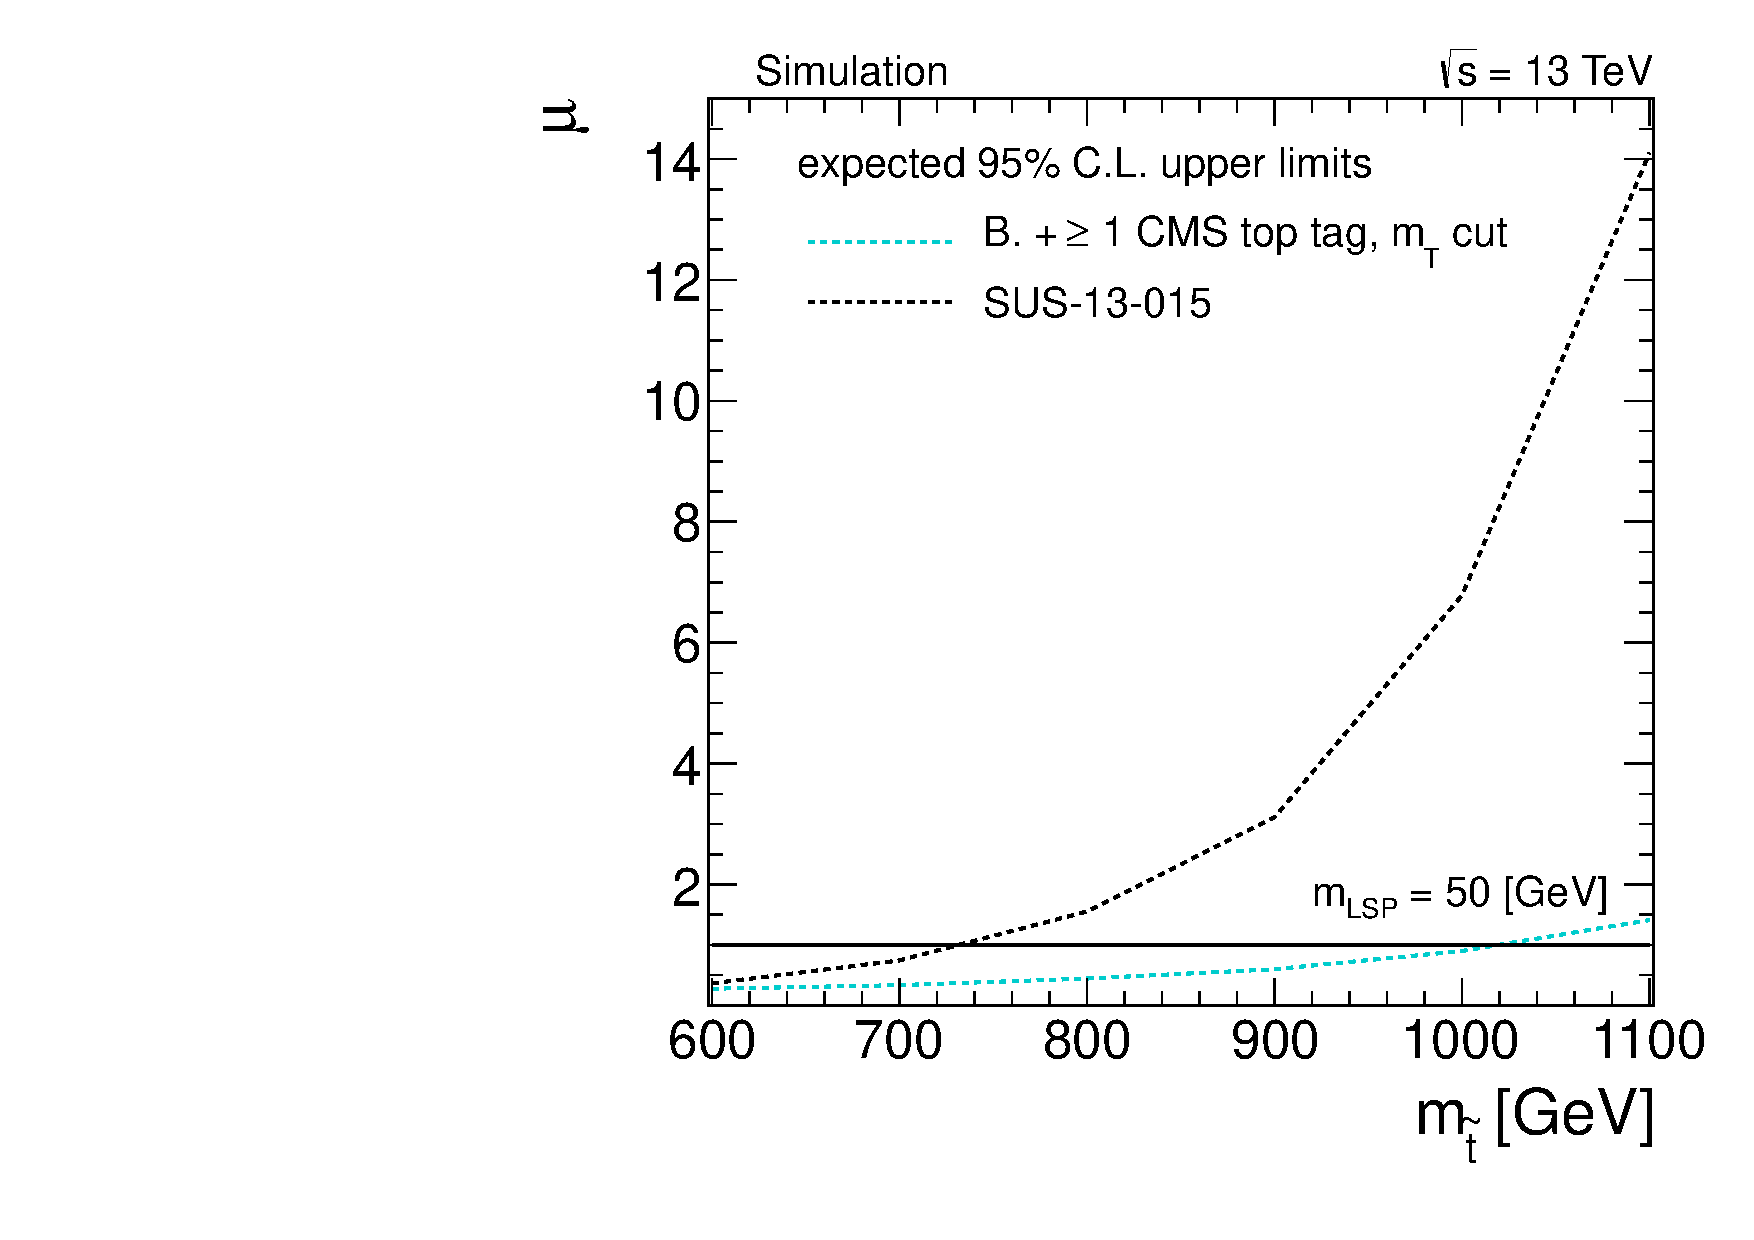
\includegraphics[width=0.49\textwidth]{figures/limitplot4BinSel_BaselineTopTagTransverseMassRef_LSP50.pdf} 
  \end{tabular}
  \caption{Expected 95\% upper limit for signal strength versus $m_{\tilde{t}}$. The LSP mass is chosen to be 50\gev. The label B. denotes the baseline selection.}
  \label{fig:stop_baselinetoptagref_limit}
\end{figure}
The limit curves exhibit that the selection based on the requirements used in SUS-13-015 shows a quite good sensitivity for low stop masses while the sensitivity drops rapidly towards higher stop masses. However, the selection proposed in Sec.~\ref{sec:stop_cuts} performs better for all mass scenarios.  

%\section{Studies of Alternative Selections}
%\label{sec:stop_alternatives}
%As discussed in Sec.~\ref{sec:stop_pub}, a selection developed in the context of this thesis could be identified that is well suited to probe stop masses up to the \tev range for an LSP mass of 50\gev at $\sqrt{s} = 13$\tev and performs even better than the selection criteria developed for the search for direct stop quark production at $\sqrt{s} = 8$\tev. However, it is discussed in this section which specific criteria of the studied selections leave further room for improvement and how alternative selections might be better suited to probe specific regions of the phase space. \\
%The evolution of the signal efficiency as function of the stop quark mass for a LSP mass of 50\gev is shown in Fig.~\ref{fig:stop_signal efficiency} for the application of different selection criteria. 
 
%\begin{figure}[!t]
%  \centering
%  \begin{tabular}{c}
%                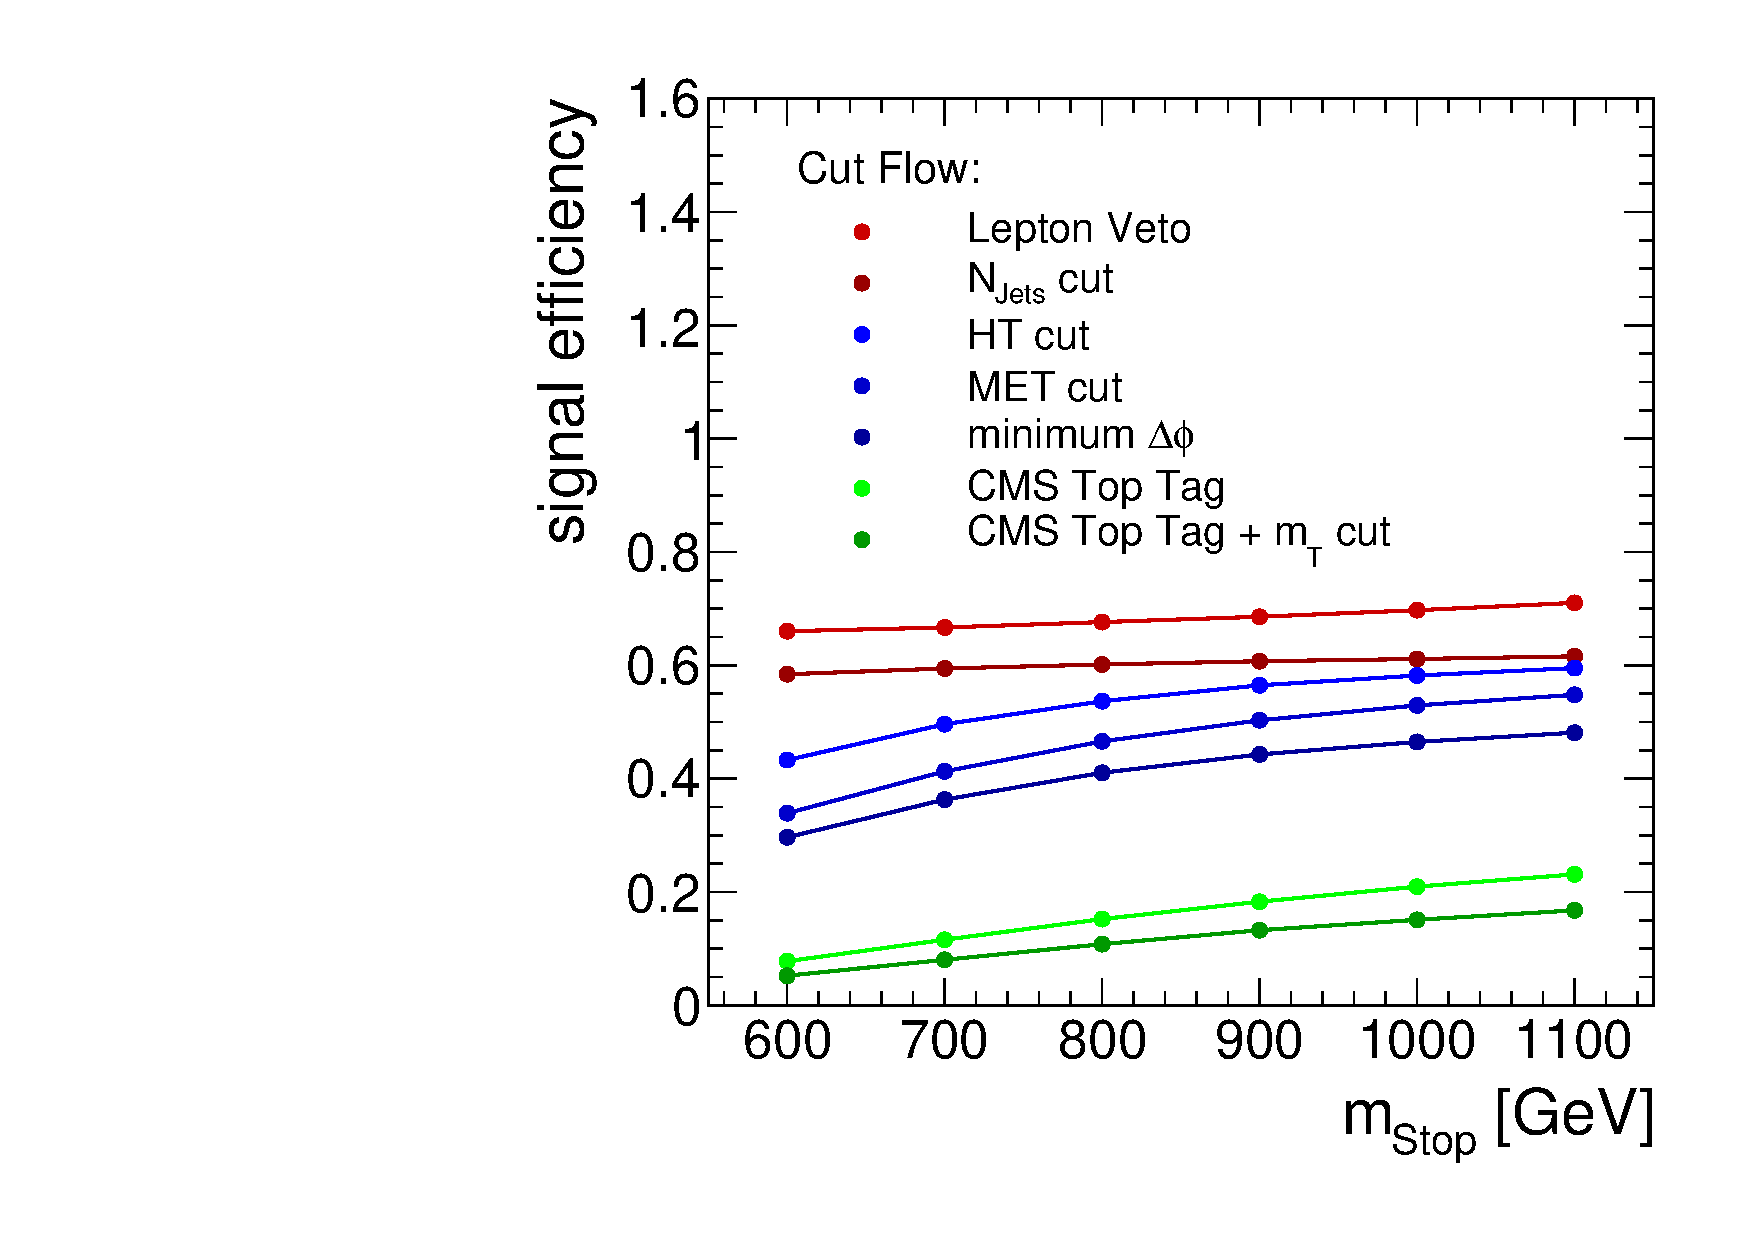
\includegraphics[width=0.49\textwidth]{figures/SignalEfficiencySummary.pdf} 
%  \end{tabular}
%  \caption{Signal efficiency as function of the stop quark mass for a LSP mass of 50\gev for various selection requirements.}
%  \label{fig:stop_signal efficiency}
%\end{figure}

\section{Stability Test}
\label{sec:stop_syst}
In order to study the stability of the sensitivity of the identified selection towards the assumed background uncertainties, the expected limit for the selection using the baseline requirements, at least one CMS top tag and $m_\mathrm{T} > 180$\gev is evaluated when varying the assumed \ttbar uncertainty. \\
%The behaviour concerning the binning of the search regions is studied by dividing the region $ 200 < \met < 400$\gev into two: $ 200 < \met < 300$\gev and $ 300 < \met < 400$\gev. Here, the systematic uncertainties are considered as before. \\
The dependence on the assumed uncertainties is studied by increasing the uncertainties considered for \ttbar from 20\% to 50\% while others stay unchanged. Since for this selection \ttbar is the main background, the variation of the \ttbar uncertainty is expected to cause the largest deviation. 
The expected limits derived using the nominal and the increased \ttbar uncertainty are illustrated in Fig.~\ref{fig:stop_varied_limit}. It turns out that the resulting change for the sensitivity caused by this variation is small and only impacts small stop quark masses.  
\begin{figure}[!b]
  \centering
  \begin{tabular}{c}
                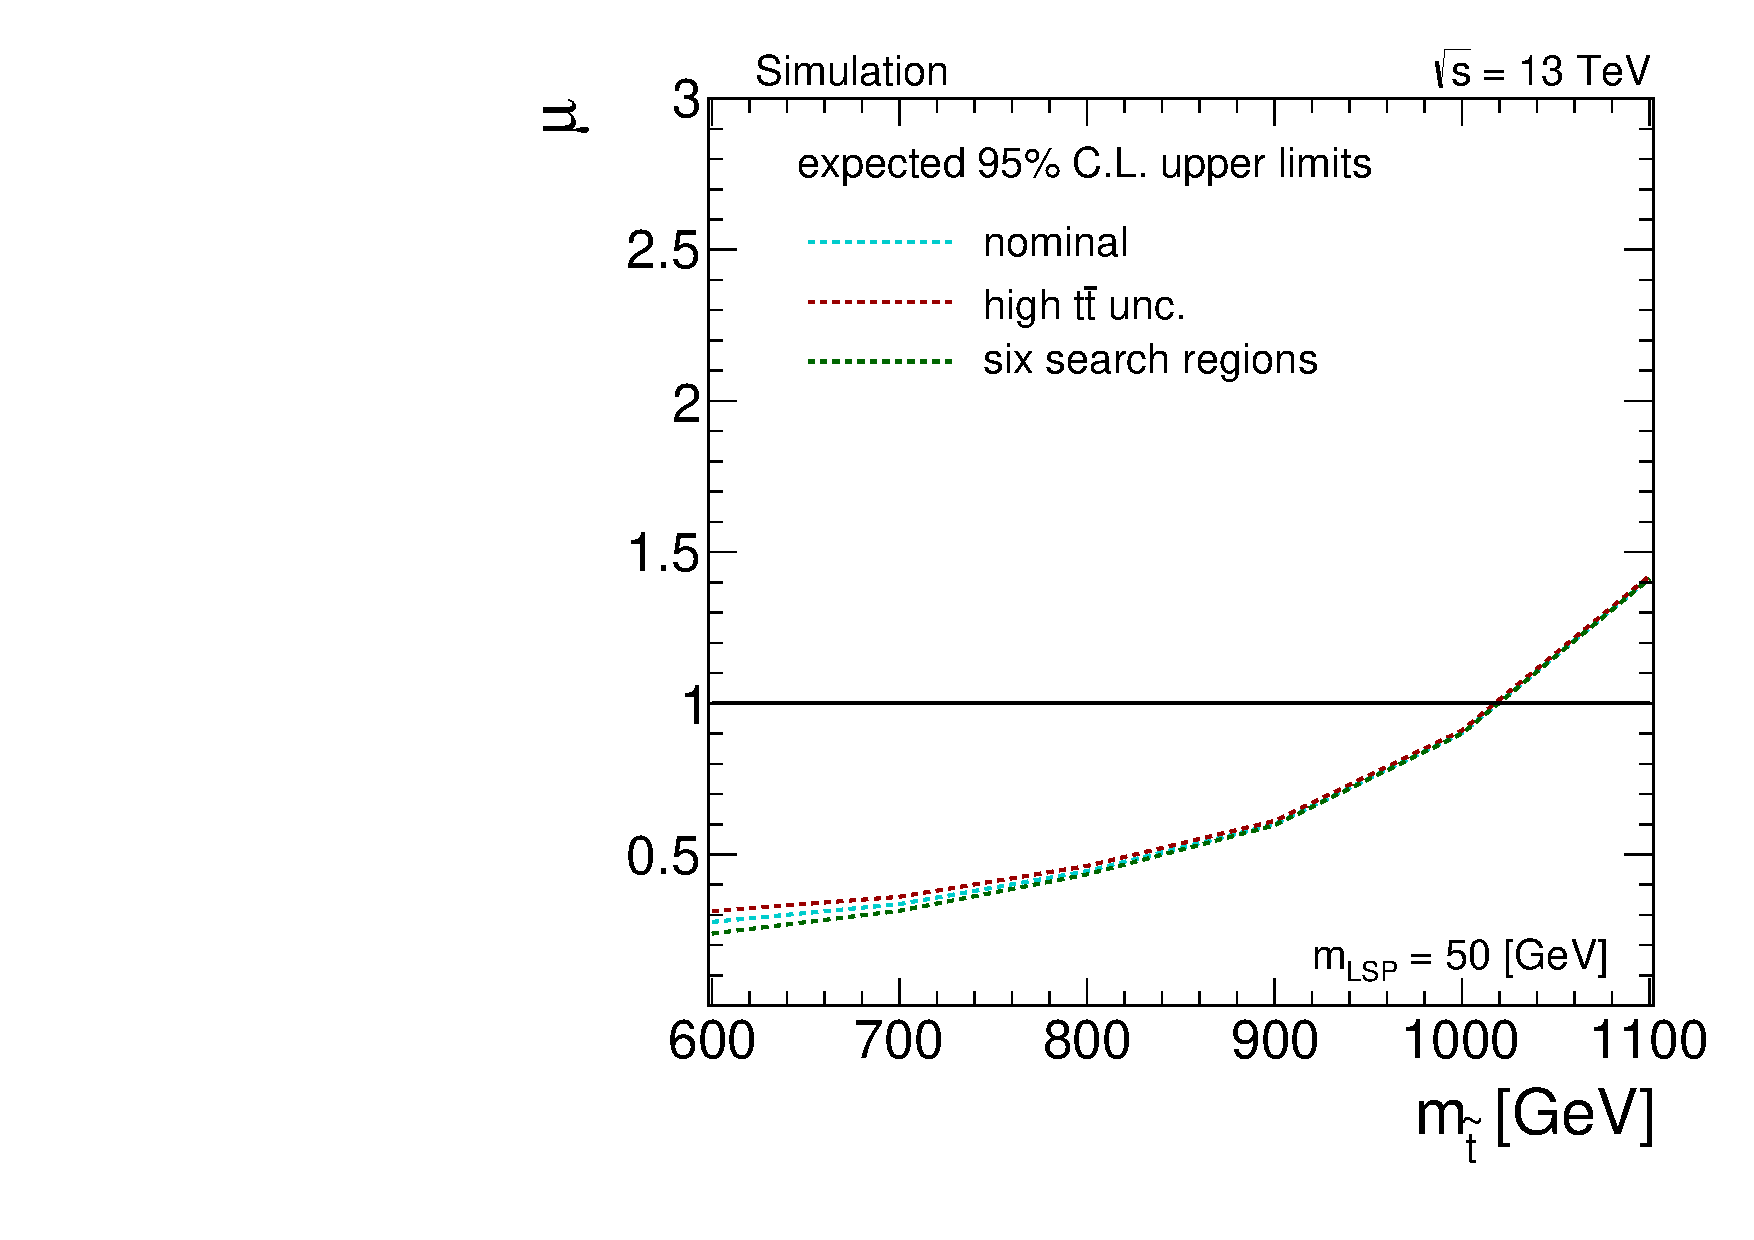
\includegraphics[width=0.49\textwidth]{figures/limitplot4BinSel_SystVariation_LSP50.pdf} 
  \end{tabular}
  \caption{Expected 95\% upper limit for signal strength versus $m_{\tilde{g}}$. The LSP mass is chosen to be 50\gev.}
  \label{fig:stop_varied_limit}
\end{figure}
\\
Consequently, the derived selection is able to probe the stop quark mass region up to 1\tev even for a much higher uncertainty on the \ttbar background. Accordingly, if the \ttbar background can not be determined in data to a precision of 20\%, the sensitivity of the analysis is expected to be not much degraded for the studied stop quark masses.              

\section{Sensitivity to Gluino-Mediated Stop Production}
\label{sec:stop_gluinos}
\begin{figure}[!t]
  \centering
  \begin{tabular}{cc}
  % \makebox[\linewidth]{
   
      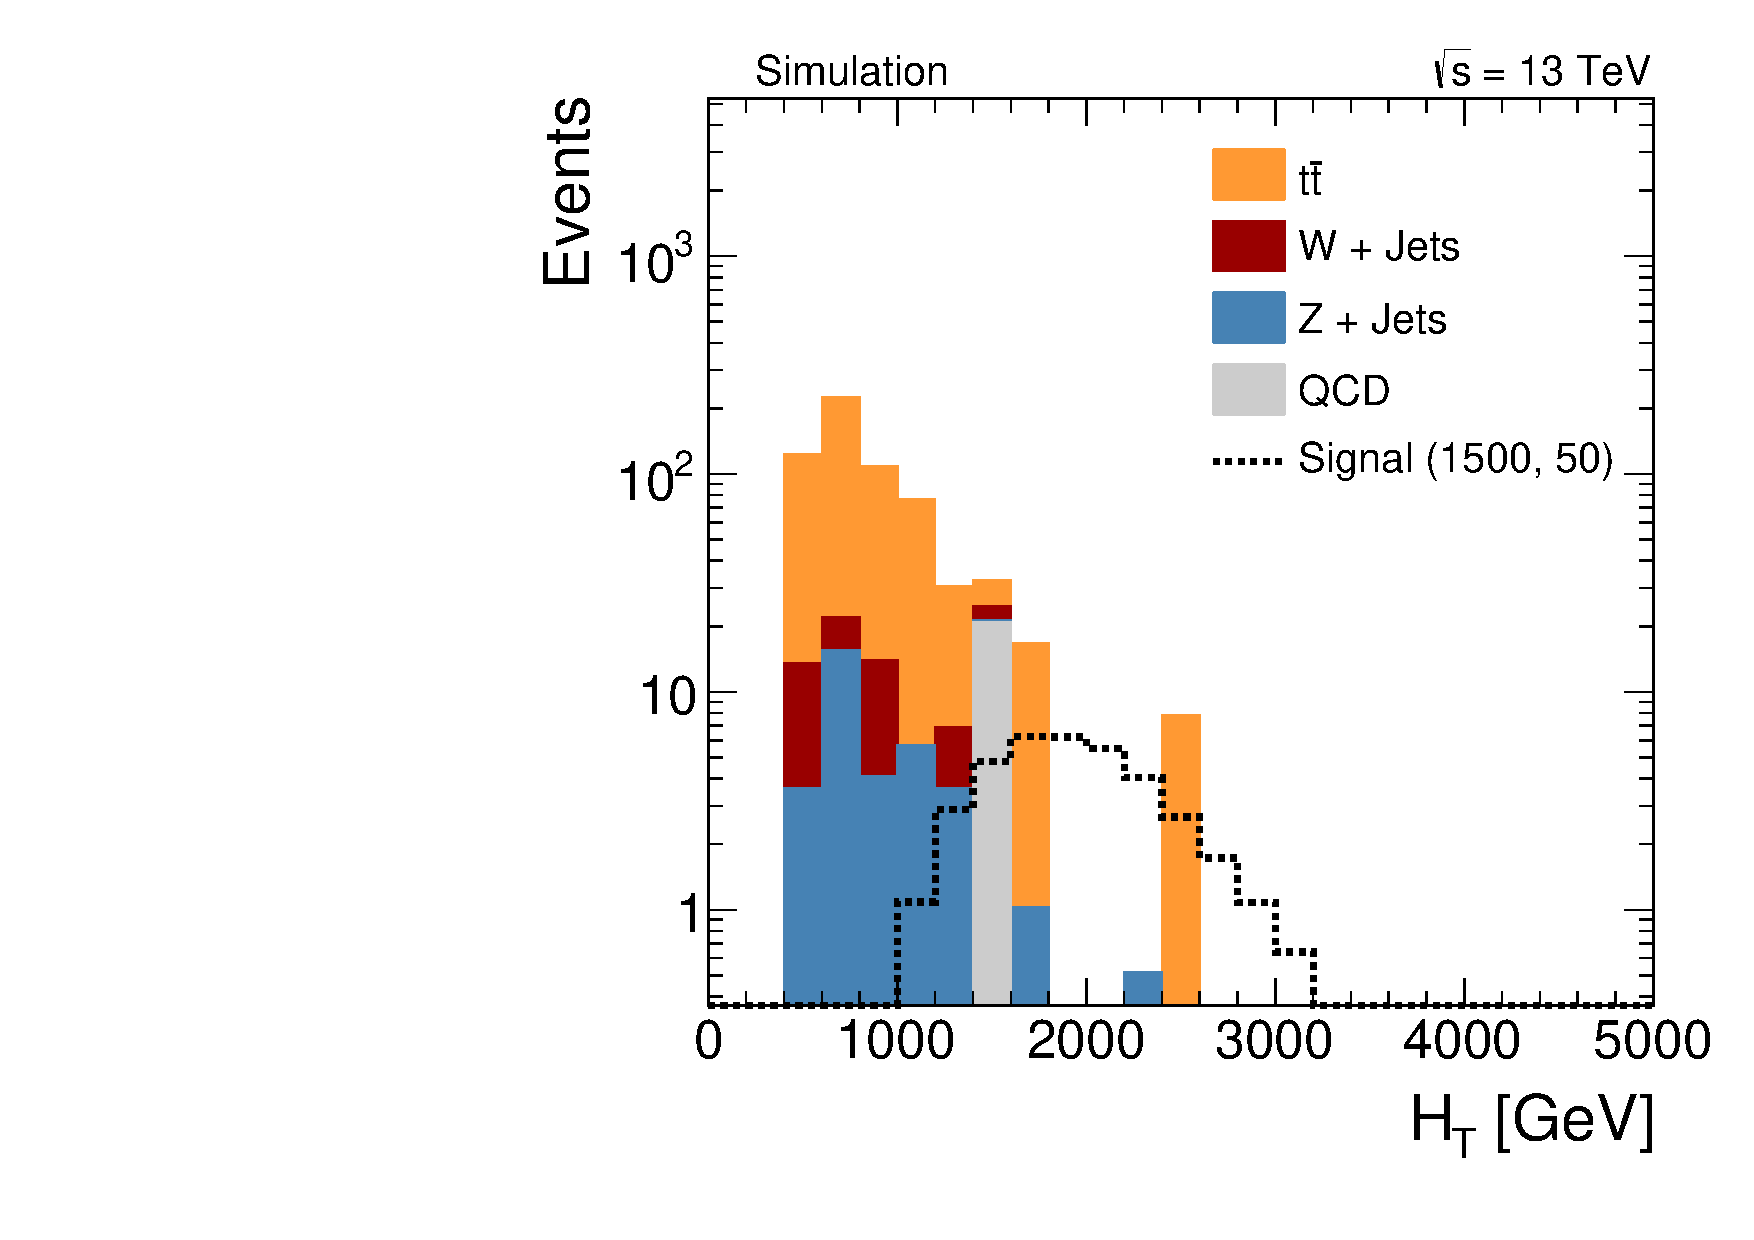
\includegraphics[width=0.49\textwidth]{figures/Stop_TopTagTransverseMass_HThad_GluinoT1tttt.pdf}  
      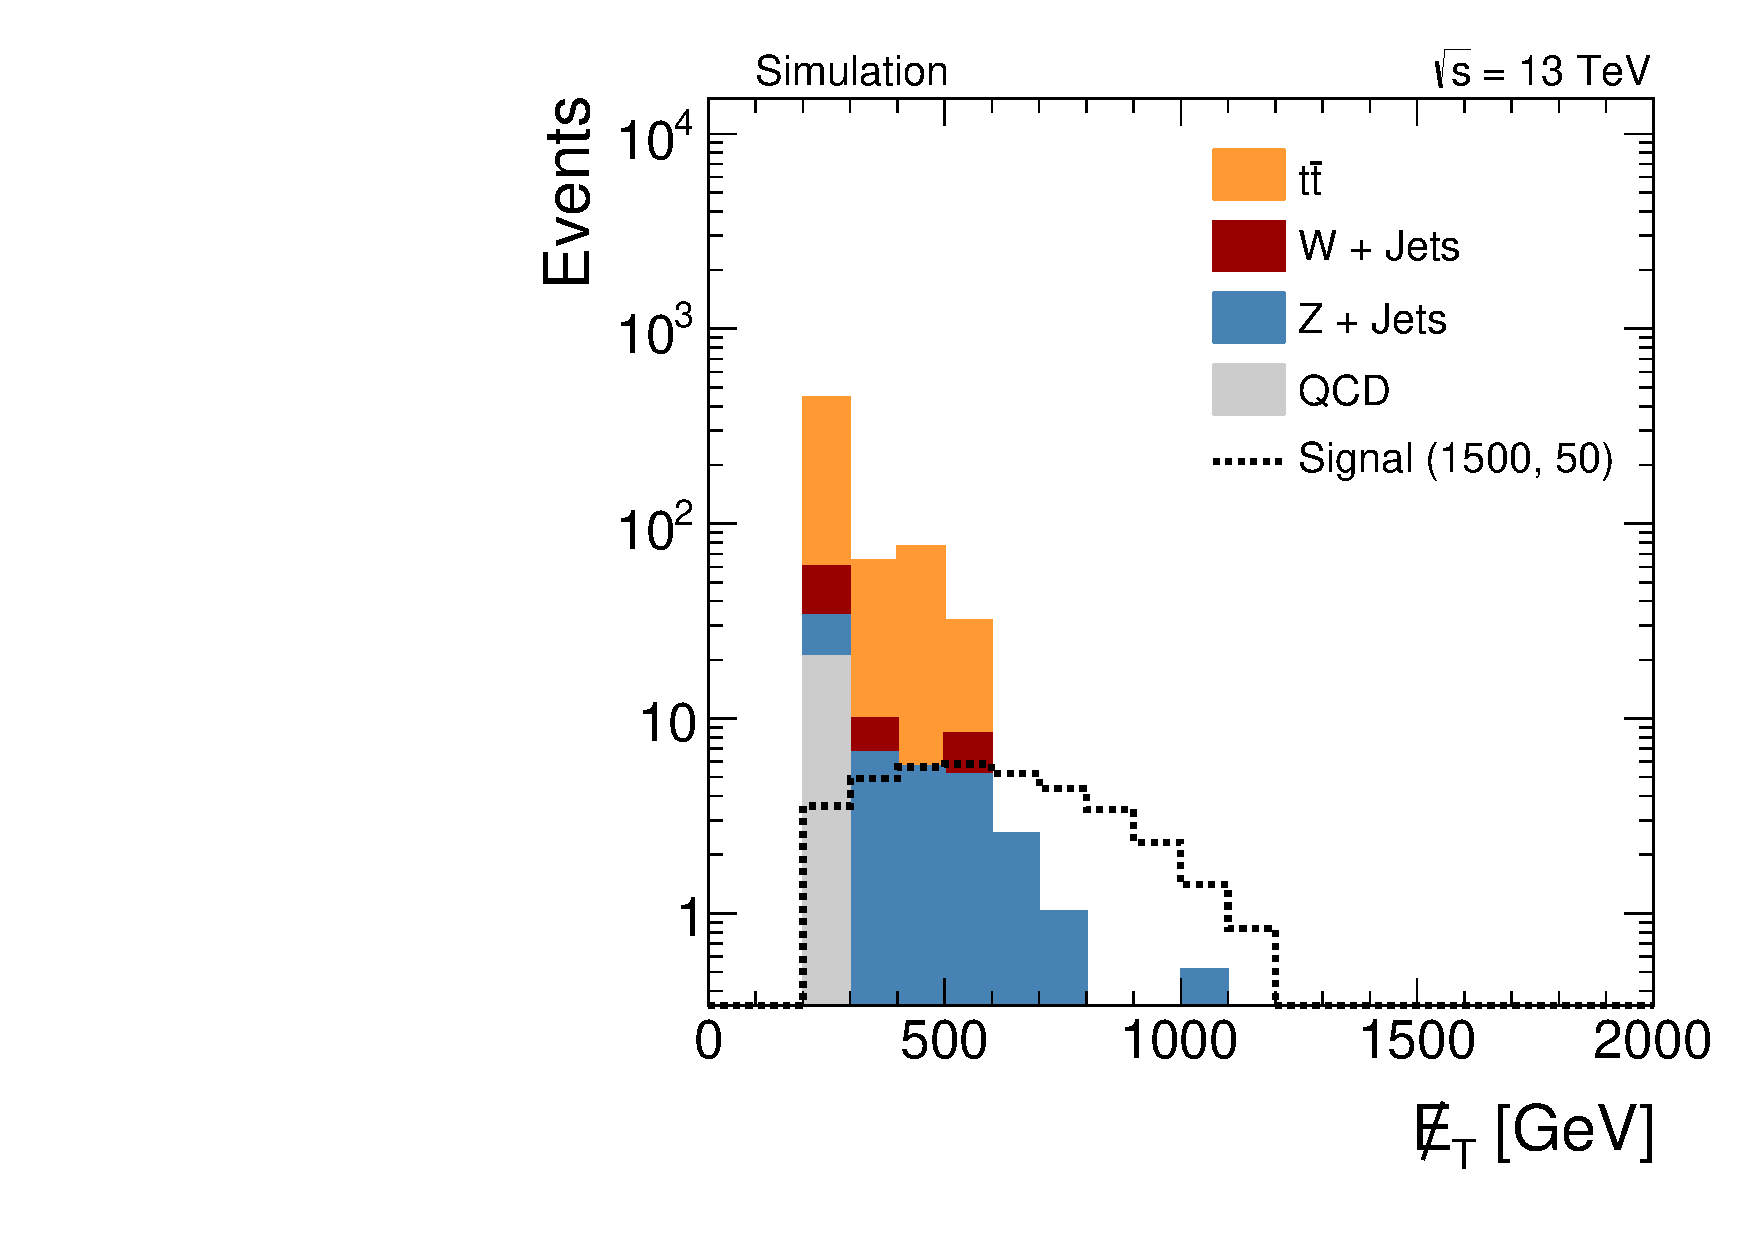
\includegraphics[width=0.49\textwidth]{figures/Stop_TopTagTransverseMass_MET_GluinoT1tttt.pdf} 
    \end{tabular}
 
  \caption{Comparison of selected \HT (\textit{left}) and \met (\textit{right}) distributions in simulated events found from applying the baseline selection criteria, at least one CMS top tag and $m_\mathrm{T} > 180$\gev. The signal points for gluino-mediated stop production are labelled as (X, Y) where X is the gluino mass and Y is the LSP mass in GeV.}
  \label{fig:stop_gluinos_ht_met}
\end{figure}
The selections studied in this chapter were developed for selecting events from direct pair production of stop quarks which each subsequently decays into a top quark and a LSP. Special emphasis is put on identifying mass scenarios with large mass splittings between stop quark and LSP which is suitable for employing top tagging techniques. However, the studied selections offer an interesting alternative to classical selections targeting gluino-mediated production of third generation squarks. In those scenarios, pair produced gluinos are considered in which each subsequently decays into a pair of top quarks and a LSP, as studied in Chap.~\ref{chap:RA2}. Thus, the final state contains four top quarks. For gluino masses exceeding 1\tev, this gives rise to boosted top quark decays in the final state. In order to study this model, the sensitivity of the best performing selection criteria based on the baseline selection, at least one CMS top-tagged jet and a transverse mass selection of $m_\mathrm{T} > 180$\gev is also evaluated with respect to the gluino-mediated stop production. A comparison of \HT and \met for one selected signal point and respective background events after applying these selection criteria is shown in Fig.~\ref{fig:stop_gluinos_ht_met}. \\
The evaluation of the sensitivity towards gluino-mediated stop production is performed for three different mass scenarios, as specified in Sec.~\ref{sec:stop_samples}, with gluino masses of 1.3\tev, 1.5\tev and 1.7\tev for a LSP mass of 50\gev, respectively. Based on the same search strategy as before, using exclusive \HT and \met search regions, the derived expected exclusion curve for gluino-mediated stop production is illustrated in Fig.~\ref{fig:stop_gluino_mediated_limit}. 
\begin{figure}[!t]
  \centering
  \begin{tabular}{c}
                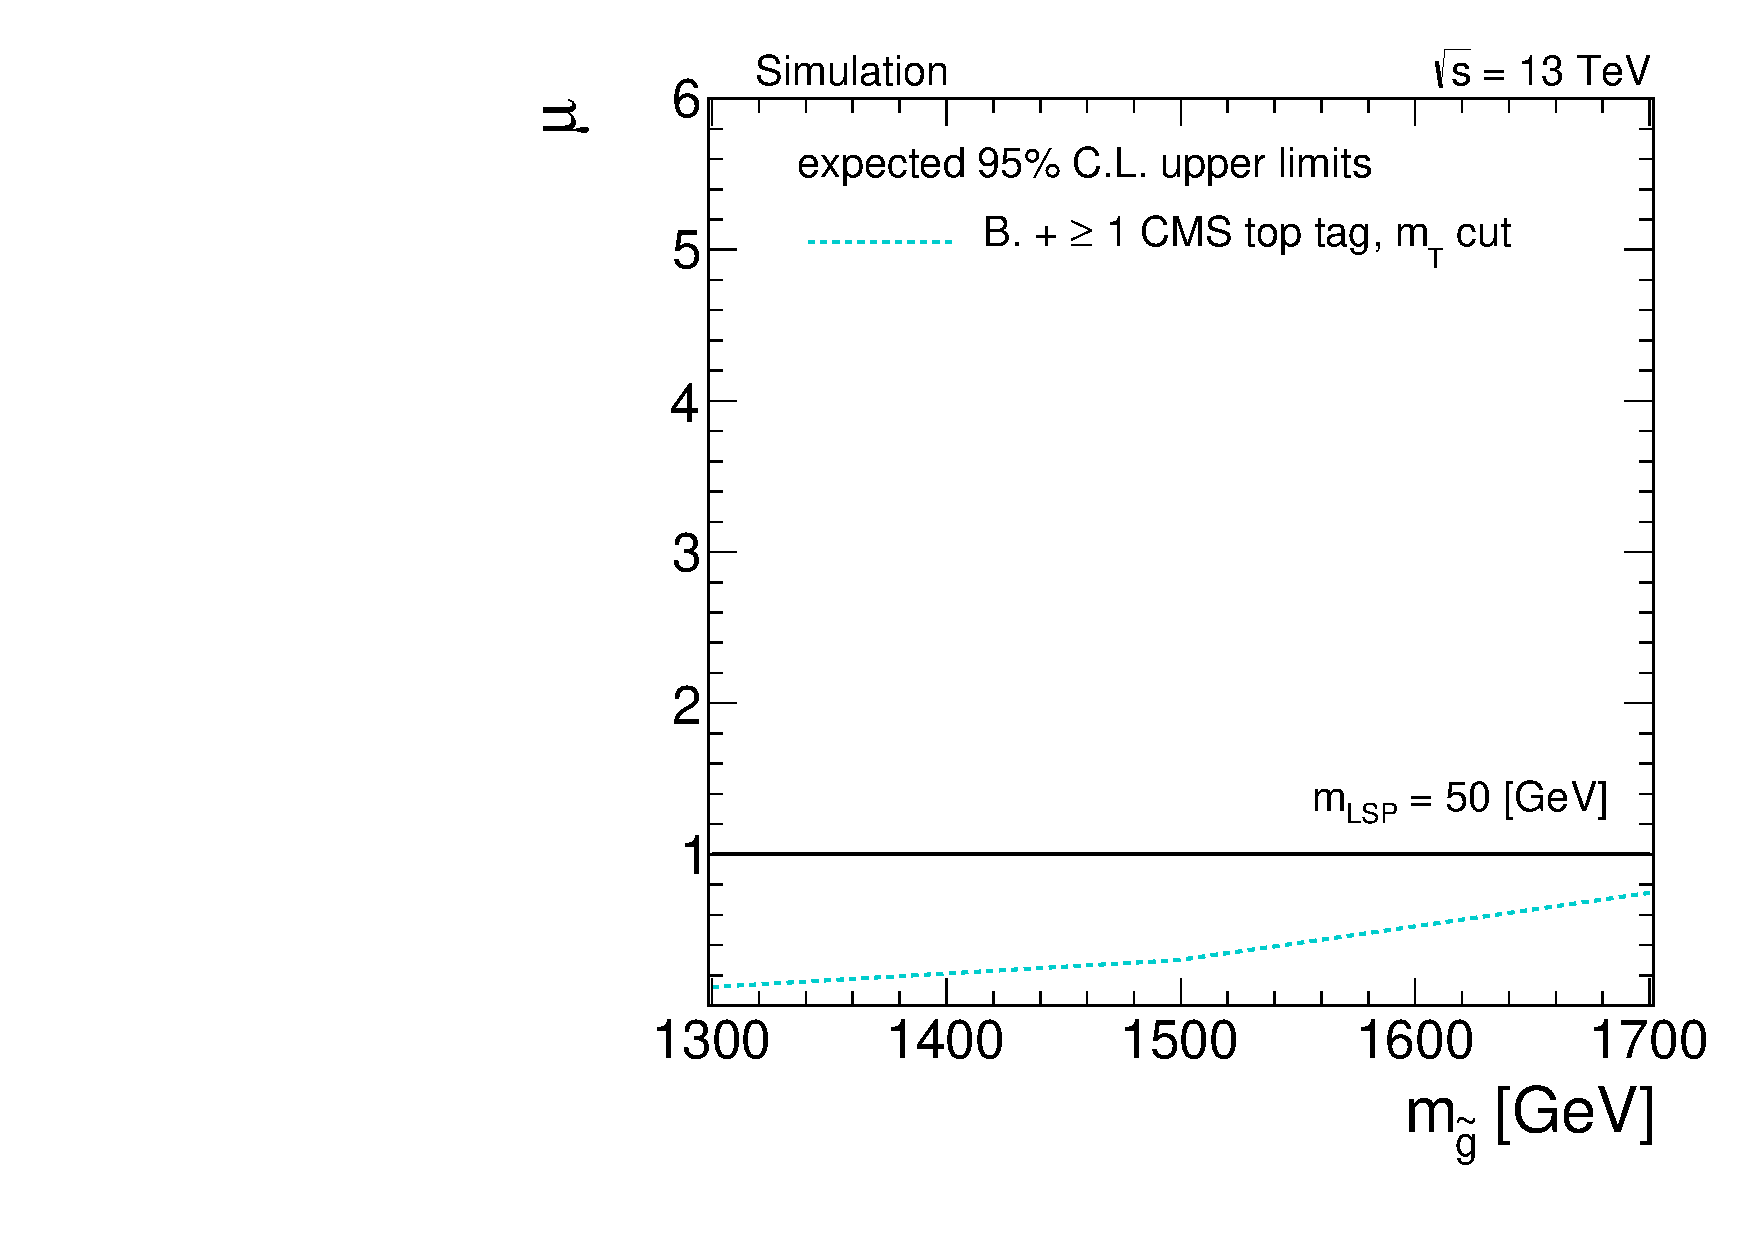
\includegraphics[width=0.49\textwidth]{figures/limitplot4BinSel_T1tttt.pdf} 
  \end{tabular}
  \caption{Expected 95\% upper limit for signal strength versus $m_{\tilde{g}}$. The LSP mass is chosen to be 50\gev. The label B. denotes the baseline selection.}
  \label{fig:stop_gluino_mediated_limit}
\end{figure}
\\
The limit curve shows that the derived selection described in Sec.~\ref{sec:stop_cuts} is also sensitive to the tested mass scenarios of gluino-mediated stop production. Thus, selections involving top tagging also offer the opportunity to probe SUSY scenarios other than direct stop production as long as top quarks with high transverse momenta are present in the final state. Such selections could serve as complementary approach to search strategies like those employed in chapter~\ref{chap:RA2} for further supersymmetry searches at $\sqrt{s} = 13$\tev. 

\section{Results and Discussion}
\label{sec:stop_results}
Selections based on different kinematic properties of direct stop pair production have been studied and analysis strategies were identified that allow to probe direct stop production up to 1\tev in case of an LSP mass of 50\gev (cf. Sec.~\ref{sec:stop_cuts}). However, the sensitivity of this selection targeting large mass splittings between stop and LSP can be evaluated also for other mass scenarios. For illustration, the selected \HT and \met distributions for the baseline selection, at least one CMS top tag and $m_\mathrm{T} > 180$\gev are shown in Fig.~\ref{fig:stop_highLSP_ht_met} for a stop mass of 900\gev and a LSP mass of 50\gev and 350\gev, respectively. As expected, the spectra for the larger mass difference of stop quark and LSP are harder than in the case that the mass difference is smaller. However, both variables still provide separation power such that the same selection is expected to provide sensitivity also to various scenarios with smaller mass splittings. 
\begin{figure}[!t]
  \centering
  \begin{tabular}{cc}
  % \makebox[\linewidth]{
   
      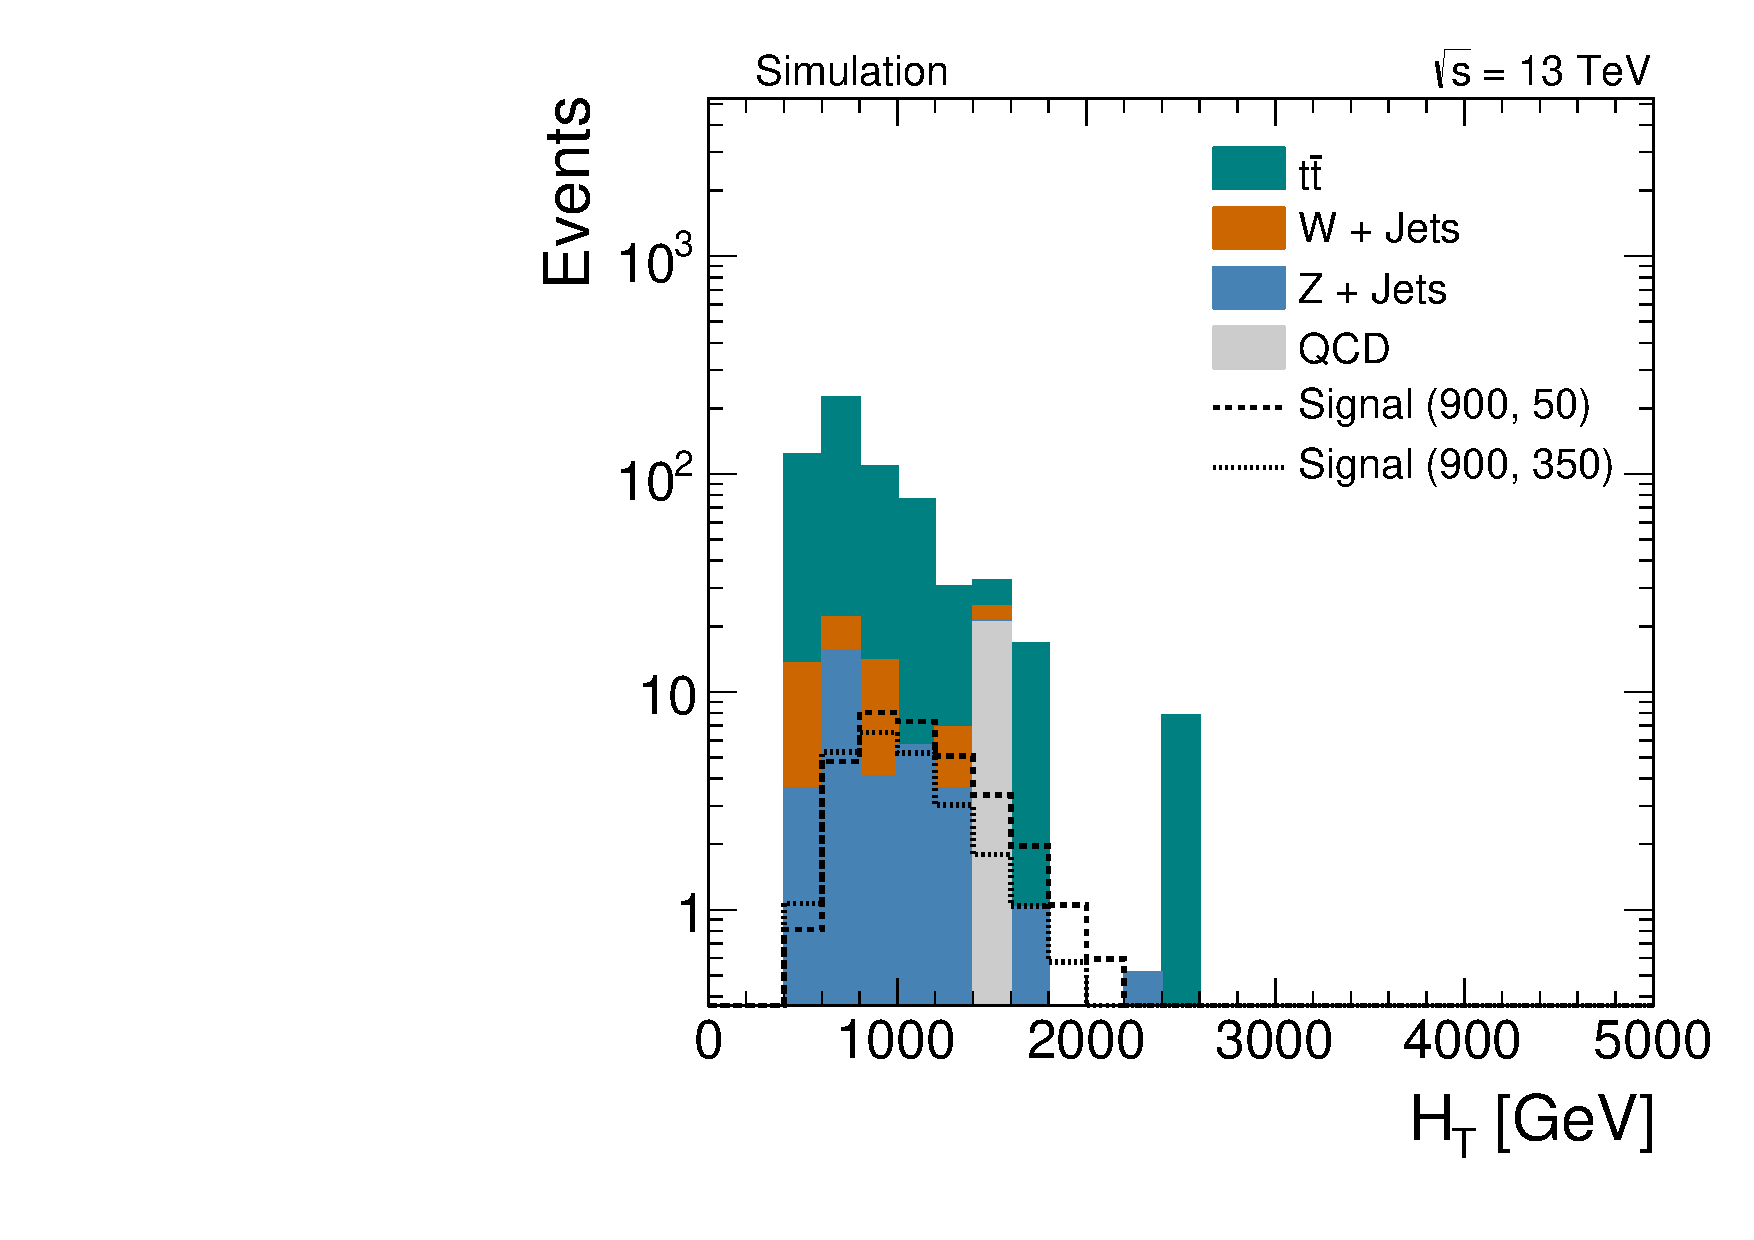
\includegraphics[width=0.49\textwidth]{figures/Stop_TopTagTransverseMass_HThad_HighLSPMass.pdf}  
      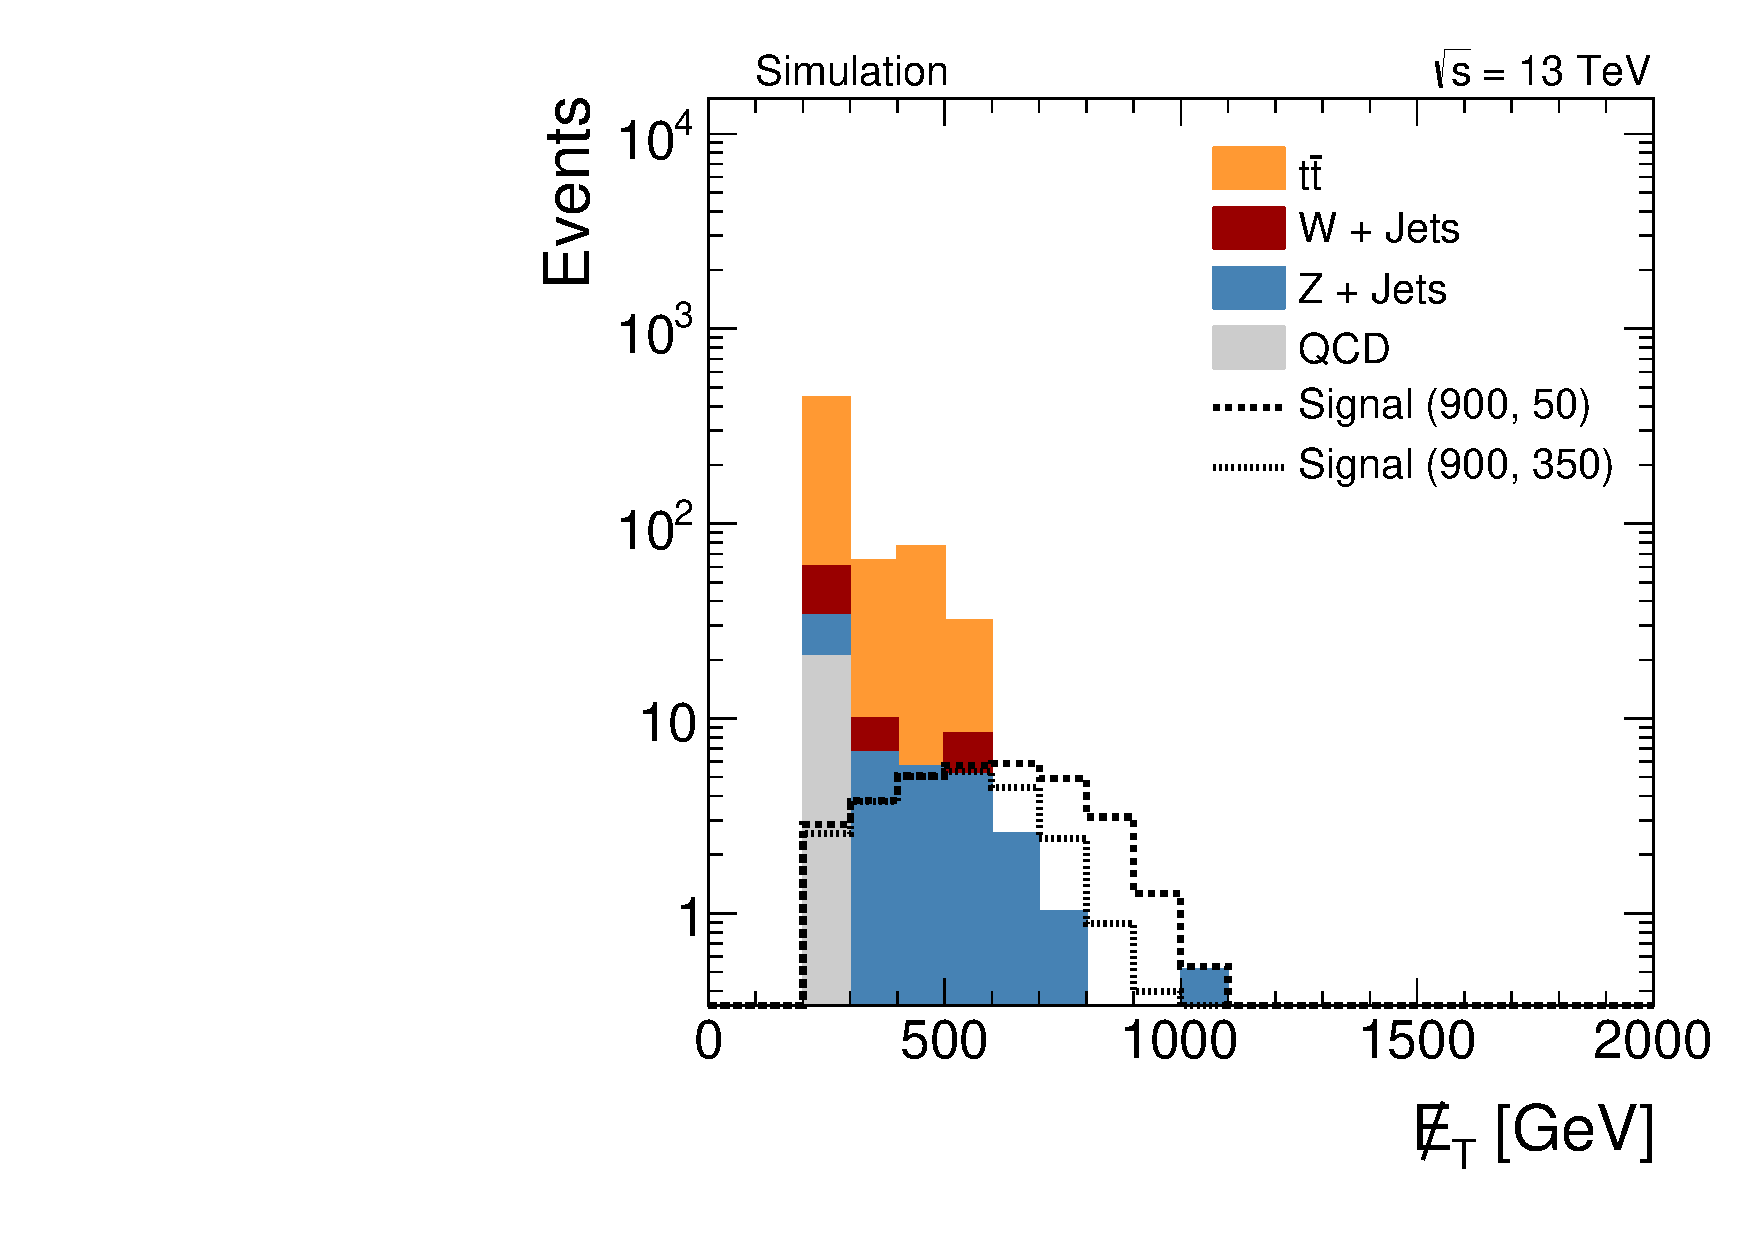
\includegraphics[width=0.49\textwidth]{figures/Stop_TopTagTransverseMass_MET_HighLSPMass.pdf} 
    \end{tabular}
 
  \caption{Comparison of selected \HT (\textit{left}) and \met (\textit{right}) distributions in simulated events found from applying the baseline selection criteria, at least one CMS top tag and $m_\mathrm{T} > 180$\gev. The signal points for direct stop production are labelled as (X, Y) where X is the stop mass and Y is the LSP mass in GeV.}
  \label{fig:stop_highLSP_ht_met}
\end{figure}
\\
Thus, the same search strategy and assigned uncertainties have been used to probe the expected exclusion reach for the same stop masses as before but when considering the LSP mass to be larger. Here, LSP masses up to 350\gev are considered. The derived exclusion curves are summarized in Fig.~\ref{fig:stop_2Dlimit} in the $m_{\tilde{t}}$ versus $m_\mathrm{LSP}$ plane. The illustrated selections are on the one hand baseline requirements adding at least one CMS top tag and $m_\mathrm{T} > 180$\gev (light blue) discussed in Sec.~\ref{sec:stop_cuts} and on the other hand the selection based on SUS-13-015 discussed in Sec.~\ref{sec:stop_pub} (black). The areas below the lines can be excluded. In particular for the selection indicated by the light blue line, stop masses up to 1\tev can be tested for LSP masses not exceeding 300\gev. \\
In general, the conclusions found in previous sections also hold for the two dimensional exclusion curves: The best sensitivity for a wide range of mass point configurations is achieved by the selection introduced in Sec.~\ref{sec:stop_cuts}. Although the selection following SUS-13-015 is able to probe stop masses up to 700--800\gev also for other LSP masses than 50\gev, the sensitivity towards larger stop masses is not achieved. These studies suggest that in order to test the whole stop mass range up to 1\tev a search strategy as proposed in this chapter can be employed. 
\\
Nonetheless, it has to be kept in mind that the studies shown here, have been made with some simplified assumptions, as introduced in Sec.~\ref{sec:stop_samples}. The pileup scenario considered in the simulation is not the actual expected situation during the next running period, but uses the pileup conditions form $\sqrt{s} = 8$\tev. As discussed already in Sec.~\ref{sec:stop_samples}, this should in principle not affect the analysis shown here too much. Furthermore, the samples have been processed based on the fast detector simulation only. Although this has shown a comparable performance to the full simulation for several quantities in the past, as discussed in Sec.~\ref{sec:sim_detector}, no dedicated studies have been performed yet if those holds also for all jet substructure variables used for the top tagging algorithms. Nevertheless, the derived efficiency and misidentification rates illustrated in Fig.~\ref{fig:stop_top_eff} show a similar performance to those quantities at $\sqrt{s} = 8$\tev (cf. Sec.~\ref{sec:boosted_tops}). Consequently, the performance improvement of the analysis due to an employment of top tagging is expected to be estimated at the correct order of magnitude. In addition to those simplifications, also the considered uncertainties for the different background processes are based on ad hoc assumptions. Although they have been chosen in correspondence to the considered uncertainties in~\cite{CMS-PAS-SUS-13-015}, it is not yet studied how precisely the individual background contributions can be estimated for the extreme kinematic regions targeted by the top tagging selections when employing a data-based background estimation procedure which still has to be defined. Thus, the absolute expected analysis reach might be better or worse by some 10\gev than found in these studies. However, as stated in Sec.~\ref{sec:stop_samples} the main goal of the studies was to identify general concepts and suitable selection criteria. Since it is expected that employed simplifications affect the various selections studied in this chapter in a similar manner, the sensitivity of the selections relative to each other is reflected correctly. Hence, the general conclusions stay valid and data at $\sqrt{s} = 13$\tev can be utilized to shed light on the question if there is a realization of supersymmetry manifesting in stop quarks below the TeV mass range when employing selections introduced in this thesis.  
\begin{figure}[!t]
  \centering
  \begin{tabular}{c}
                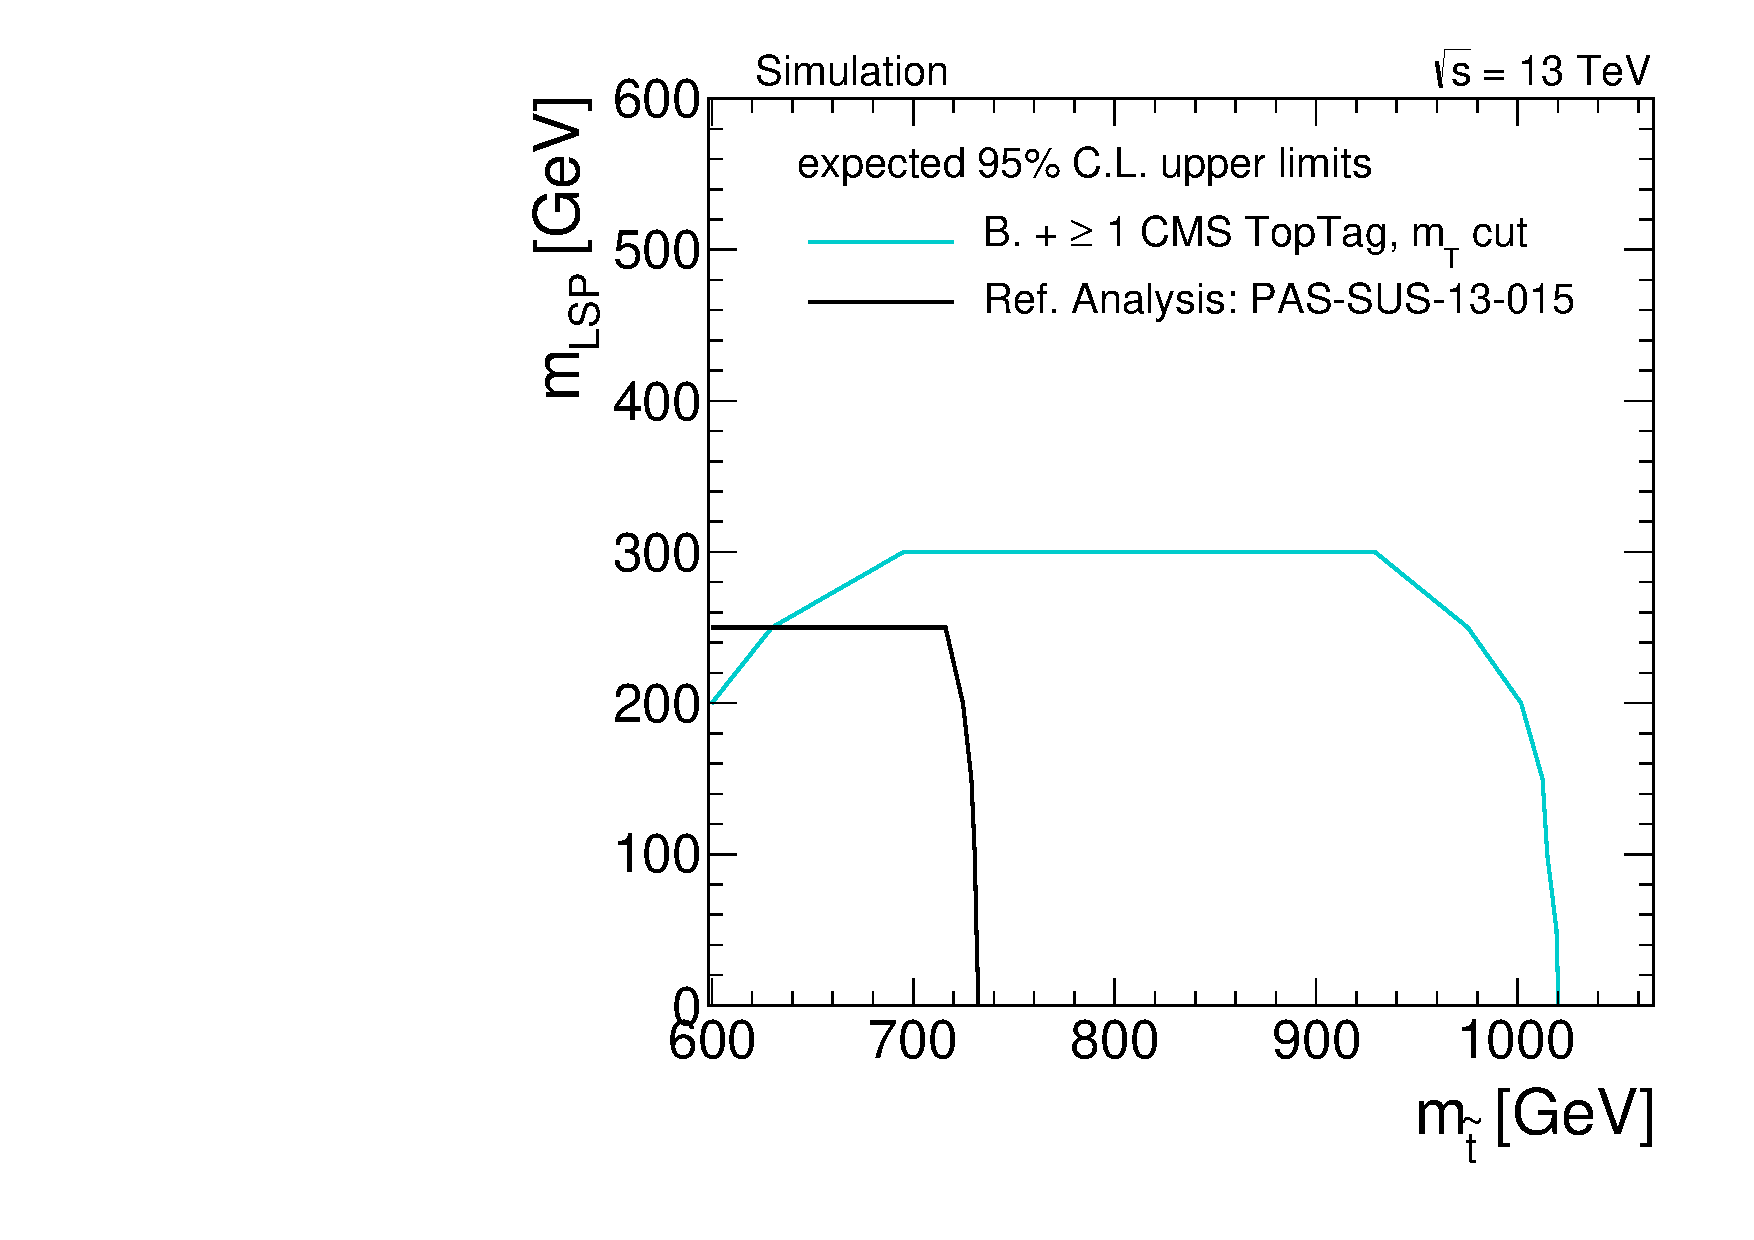
\includegraphics[width=0.49\textwidth]{figures/2Dlimitplot.pdf} 
  \end{tabular}
  \caption{Expected 95\% upper limit for $m_{\tilde{t}}$ versus $m_\mathrm{LSP}$. The label B. denotes the baseline selection.}
  \label{fig:stop_2Dlimit}
\end{figure} 

